% !TEX encoding = UTF-8 Unicode
\documentclass[12pt, a4paper]{report}
\usepackage{functan}
\usepackage{centernot}
\usepackage{fontspec}
\usepackage{polyglossia}
\usepackage{underscore}
\setdefaultlanguage{russian}
\usepackage[cm]{fullpage}
\usepackage{latexsym}
\usepackage{amsthm}
\usepackage{amsmath}
\usepackage{amssymb}
\usepackage{mathtools}
\usepackage{dsfont}
\usepackage{esint}
\usepackage{mathrsfs}
%\usepackage[parfill]{parskip}
\usepackage{pgfplots}
\usepackage{graphicx}
\pgfplotsset{compat=1.12} 

\graphicspath{ {illustrations/} }

\setmainfont[Mapping=tex-text]{CMU Serif}

\newcommand{\real}{\mathds{R}}
\newcommand{\complex}{\mathds{C}}
\newcommand{\linop}{\mathscr{L}}
\newcommand{\dsint}{\displaystyle \int}
\newcommand{\intO}{\int \limits_{\Omega}}
\newcommand{\eps}{\varepsilon}
\newcommand{\ssubset}{\subset\joinrel\subset}
\newcommand{\beauD}{\mathscr{D}}
\newcommand{\unicom}{\overrightarrow{\rightarrow}}
\newcommand\pder[2][]{\ensuremath{\frac{\partial#1}{\partial#2}}} 
% гамильтониан - \nabla
% лапласиан - \Delta
% даламбертиан - \square

\DeclareMathOperator{\esssup}{ess\,sup}
\DeclareMathOperator{\supp}{supp}
\DeclareMathOperator{\grad}{grad}
\DeclareMathOperator{\const}{const}
\DeclareMathOperator{\diam}{diam}
\DeclareMathOperator{\Ker}{Ker}
\DeclareMathOperator{\Div}{div}
\DeclareMathOperator{\Span}{span}
\DeclarePairedDelimiter\abs{\lvert}{\rvert}
\DeclarePairedDelimiter\action{<}{>}

\newtheorem{theorem}{Теорема}
\newtheorem{prop}{Предложение}
\newtheorem*{lemma}{Лемма}
\newtheorem*{corollary}{Следствие}

\theoremstyle{definition}
\newtheorem{definition}{Определение}
\newtheorem*{example}{Пример}
\newtheorem*{examples}{Примеры}

%\theoremstyle{remark}
\newtheorem*{note}{Замечание}
\newtheorem*{reminder}{Напоминание}
\newtheorem*{exercise}{Упражнение}

%макро для второй части
\Macro{L2}{L^2}
\Macro{H1}{H^1}
\Macro{H01}{H_0^1}
\Macro{L2Om}{L^2(\Omega)}
\Macro{H1Om}{H^1(\Omega)}
\Macro{H01Om}{H_0^1(\Omega)}
\Macro{C0iOm}{C_0^\infty(\Omega)}


\begin{document}

\title{Конспект лекций по уравнениям математической физики}
\author{Лектор: Степанов Евгений Олегович}
%\date{Математико-механический факультет СПбГУ \\ Весенний семестр, 2016 г.}

\maketitle

% !TEX encoding = UTF-8 Unicode
% лекции 1-2, 13 февраля 2016
% вопросы 1-5
% 1. Однородное линейное транспортное уравнение с постоянными коэффициентами, его физический смысл (задача о распространении пятна загрязнения в канале). Решение однородного уравнения методом характеристик. Бегущая волна.
% 2. Неоднородное линейное транспортное уравнение
% 3. Основная лемма вариационного исчисления для непрерывных функций.
% 4. Основная лемма вариационного исчисления для локально интегрируемых функций
% 5. Вывод уравнения колебания струны (вариационный принцип)

\chapter*{Введение}
Курс рассчитан на один семестр и делится на две части.

Первая - классическая, она относится скорее к 19ому веку. Будет рассмотрено несколько конкретных физических моделей, соответствующие уравнения в частных производных будут выведены и решены для некоторых частных случаев.

Вторая часть более современная, и, скорее всего, она окажется концепутально новой. По крайней мере для одной задачи будет получено общее решение, будет доказано существование решения и предложено сходящееся численное решение.

\pagebreak

\section*{Обозначения, некоторые определения и используемые факты}
\begin{enumerate}
\item $\real^n$ - евклидово пространство.
\item $\abs{x}$ - евклидова норма $x$ из $\real^n$.
\item Область - открытое множество в $\real^n$.
\item Если где-то написано $\overline{\Omega}$, то $\Omega$ - ограниченная область.
\item $C(\overline{\Omega})$ - пространство непрерывных функций на $\overline{\Omega}$ с $\infty$-нормой: $\sup \{ \abs{f(x)} : x \in \overline{\Omega} \}$.
\item $L^p (\Omega)$ - пространство с нормой Гёльдера, $1 \leq p \leq \infty$.
\item $L^\infty (\Omega)$ - пространство существенно ограниченных функций.
\item $C^k(\overline{\Omega})$ - все частные производные до порядка $k$ включительно существуют и непрерывны вплоть до границы.
\item $C(\Omega)$ - функции, непрерывные на $\Omega$, не вплоть до границы. Не является нормированным пространством.
\item Носитель функции - замыкание множества, на котором функция не равна $0$. Носитель функции $f$ обозначается $\supp f$.
\item Финитная функция - функция с компактным носителем.
\item $C^k_0(\Omega)$ - финитные $k$ раз гладкие функции.
\item $K \ssubset \Omega$ - K относительно компактно в $\Omega$.
\item $\abs{\Omega}$ - мера области $\Omega$
\item $\displaystyle \fint \limits_{\Omega} f(x) dx = \frac{1}{|\Omega|} \int \limits_{\Omega} f(x) dx$ - интегральное среднее значений $f$ на области $\Omega$.
\item $\displaystyle \nabla = (\frac {\partial} {\partial x_1}, ... , \frac {\partial} {\partial x_n}) $ - оператор набла.
\item $\displaystyle \nabla_x u(t,x)  = \nabla u = (\frac {\partial u} {\partial x_1}, ..., \frac {\partial u} {\partial x_n}) = (u_{x_1}, ..., u_{x_n}) = \grad u $.
\item $\displaystyle \Delta = \nabla \cdot \nabla = \nabla^2$ - лапласиан.
\item $\displaystyle \Delta u = \sum \limits_{i=1}^n \frac {\partial^2 u} {\partial x_i^2}$.
\item $\displaystyle \abs {\nabla u}^2 = \sum u_{x_i}^2$.
\item $\displaystyle \Div F = \nabla \cdot F = \frac {\partial F1} {\partial x_i} + ... + \frac {\partial F_n} {\partial x_n}$ - дивергенция векторного поля $F$.
\item $\square_v u = \square u = u_{tt} - v^2 \Delta u$ - даламбертиан.

\end{enumerate}

\chapter{}
\section{Задача о распространении пятна загрязнения в канале}
Рассмотрим ситуацию: имеется водоём. В него было сброшено некоторое количество загрязняющего вещества.
Для простоты в качестве водоёма будем рассматривать реку или канал. Пренебрегаем тем, что происходит между берегами. Нас интересует, как загрязнение распространяется в длину, поэтому реку считаем одномерным объектом.

Обозначим через $c (t, x) $ концентрацию загрязняющего вещества в момент $t \in \real_+$ в точке $x \in \real$. Пусть дана функция $ c_0 (x) $, описывающая концентрацию вещества в начальный момент времени $ t = 0 $:
$$ c_0 (x) = c (0, x).$$
% функция линейна
Задача состоит в том, чтобы описать изменение концентрации загрязняющего вещества в реке при условии, что мы что-то знаем про течение реки. Как минимум мы знаем скорость. Будем считать, что загрязняющее вещество никуда не испаряется, тогда можно воспользоваться законом сохранения массы.

\subsection{Закон сохранения массы}

Рассмотрим изменение концентрации вещества на некотором малом интервале $ [x, x + \Delta x] $:
$$ \dsint \limits_x^{x + \Delta x} c (t, \xi) d \xi .$$
Рассмотрим функцию $ q (t, x) $ - поток загрязняющего вещества в момент времени $t$ через стенку $x$. Изменение концентрации можно описать как разность величин "сколько влилось" и "сколько вылилось": 
$$ \dsint \limits_x^{x + \Delta x} c (t, \xi) d \xi = q (t, x) - q (t, x + \Delta x). $$
Будем считать, что функция $q (t, x) $ достаточно гладкая. Внесём под интеграл $ \displaystyle \frac {d} {dt} $, а потом разделим обе части на длину нашего малого интервала $ \Delta x$:
$$ \fint \limits_x^{x + \Delta x} c_t (t, \xi) d \xi  = \frac {q  (t, x) - q (t, x + \Delta x)} {\Delta x}.$$
Далее, устремим длину интервала $\Delta x$ к нулю. Получим, собственно, закон сохранения массы:
$$ c_t (t, x) = -q_x (t, x). $$

Стоит заметить, что предположения о гладкости и других нужных свойствах используемых функций это распространённый приём, используемый физиками для построения моделей. Эти условия достаточно сильны, и не всегда физическое явление можно описать достаточно хорошей функцией. В дальнейшем мы узнаем, что существуют более общие математические модели, которые лучше подходят для описания физических процессов.


Далее хочется узнать, как этот поток зависит от концентрации.

\subsection{Модели}
\subsubsection*{Чистая конвекция или чистый дрейф (транспортное уравнение)}

Допустим, скорость течения $v$ постоянна, а загрязняющее вещество мало диффундирует. То есть, загрязняющее вещество не смешивается с водой (в качестве примера можно привести сброс нефти в реку). Тогда поток вещества, проходящего через точку $x$ равен концентрации вещества умножить на скорость:
$$ q (t, x) = v c (t, x). $$
Если подставить вместо потока закон сохранения массы, то получим транспортное уравнение:
$$ c_t + v c_x = 0.$$

Полностью это уравнение называется однородным линейным транспортным уравнением с постоянными коэффициентами в одномерном случае.

\subsubsection*{Уравнение диффузии (закон Фика) или теплопроводности (закон Фурье)}

Допустим, течения нет (то есть, $ v \equiv 0 $), а загрязняющее вещество хорошо диффундирует (в качестве примера можно привести сброс стирального порошка в стоячий канал). Тогда
$$ q (t, x) = - D c_x (t, x), $$
где $D$ это некоторый коэффициент диффузии.

Это уравнение означает, что в момент времени $t$ поток через стенку $x$ пропорционален градиенту концентрации. Минус в правой части означает, что поток идёт оттуда, где концентрация больше, туда, где она меньше.

Позже мы узнаем, что эта же модель является моделью распространения тепла. В ней величина $1/D$ называется коэффициентом температуропроводности.

\subsubsection*{Уравнение конвекции-диффузии или конвекции с дрейфом (закон Фоккера-Планка)}
% на лекции больше ничего не было
% кроме того, что оно используется в computer science при моделировании (?) стохастических процессов
% но, опять же, это теорвер 
Эта модель описывает случай, когда присутствует и конвекция, и диффузия:
$$ q (t, x)  = x c - D c_x. $$
Подставив закон сохранения массы, получим:
$$ c_t + v_{cx} = D c_{xx}. $$

Помимо физики, такое уравнение часто встречается в теории вероятностей.

\subsection{Решение однородного транспортного уравнения}
Что мы имеем ввиду, когда говорим "решение"? Мы имеем ввиду классическое решение - функцию, которая при подстановке в уравнение даст верное соотношение. Для этого она должна обладать нужной гладкостью, а условия уравнения должны соблюдаться в каждой точке. Так понимали решения до тридцатых годов XX века. К сожалению, оказалось, что для дифференциальных уравнений в частных производных классическое решение - не самое лучшее, и зачастую его недостаточно.

За последний век было придумано много разных решений, обобщающих понятие классического: слабые, вязкостные, энтропийные. Немного позже мы узнаем об одном из них - слабом. Но пока что мы остановимся на уровне XIX века и будем рассматривать только классические решения.

Итак, нам нужно найти некоторую функцию, которая не только удовлетворяет транспортному уравнению, но еще и удовлетворяет начальному условию $ c (0, x) = c_0 (x) $:

\begin{align}
    \begin{cases} 
        c_t + v c_x = 0, \\
        c (0, x) = c_0 (x).
    \end{cases}
\label{transport}
\end{align}

Когда мы выводили это уравнение, мы брали небольшой промежуток реки от $x$ до $ x + \Delta x $ и смотрели, как распространяется загрязняющее вещество в нём. Теперь поступим по-другому: посмотрим, как ведёт себя каждая частица вещества в реке. Каждая частица плывёт по направлению течения со скоростью $v$. Значит, траектория каждой частицы удовлетворяет вспомогательному дифференциальному уравнению $ \dot x = v $. Каково решение этого уравнения?

\[
	x(0) = x_0,\quad \text{тогда } x(t) = x_0 + v t .
\]


Пусть $ c (t, x) $ - решение нашего транспортного уравнения. Подставим $ x(t) $ вместо $x$. То есть, каждая частица вещества двигается по закону $ \dot x = v $. Что получится, если мы посмотрим концентрацию вещества вдоль траектории этого ОДУ?

\begin{align*}
    \frac {d} {dt} c (t, x(t)) & = c_t (t, x(t)) + c_x (x, t) \cdot \dot x (t) = c_t (t, x(t)) + v c_x (t, x(t)) = 0
\end{align*}
%?????
Получается, что $ c_t (t, x(t)) = 0 $. Иначе говоря, вдоль траектории вспомогательного ОДУ функция $c$ является постоянной.


Как теперь найти $ c (t,x) $? Есть точка $ (t, x) $, требуется найти значение концентрации в ней. Смотрим, какая траектория ОДУ проходит через эту точку: через неё проходит единственная прямая. Знаем, что вдоль этой траектории $ c = const $, значит, $ c (t, x) = c_0 (x_0) $. А как выражается $ x_0 $? $ x = x_0 + v t $, значит, $ x_0 = x - vt $.
Итого $c(t,x) = c_0(x(0)) = c_0(x-vt)$.

\begin{definition} Обыкновенное дифференциальное уравнение, вдоль траекторий которого решения уравнения в частных производных постоянны, называется характеристическим.
\end{definition}

\begin{definition} Траектории характеристического уравнения называются характеристическими линиями или характеристиками.
\end{definition}

Наша задача оказалась устроена так, что через каждую точку проходит единственная характеристическая линия. Отсюда, зная начальное значение, мы нашли формулу для решения задачи Коши для транспортного уравнения.

Оформим результат рассуждений в виде теоремы.

\begin{theorem}
Пусть $c_0 \in C^1(\real)$. Тогда задача \eqref{transport} имеет единственное классическое решение $$ c (t,x) = c_0 (x - v t) .$$
\end{theorem}

\begin{tikzpicture}
\begin{axis}[
    axis lines = left,
    xlabel = $x$,
    xmin = -7,
    xmax = +14,
    ymax = 1.5,
]

\addplot [
    domain=-7:-3, 
    samples=250, 
    color=red,
]
{1/(1+e^(-10*(x+5)))};

\addplot [
    domain=-7:6, 
    samples=250, 
    color=blue,
]
{1/(1+e^(-10*(x-4)))};

\addlegendentry{$c(-3,x)$}
\addlegendentry{$c(7,x)$}

\addplot [
    domain=-3:-1, 
    samples=5, 
    color=red,
]
{1};

\addplot [
    domain=-1:14, 
    samples=250, 
    color=red,
]
{1/(1+e^(-10*(-x+1)))};

\addplot [
    domain=6:8, 
    samples=5, 
    color=blue,
]
{1};

\addplot [
    domain=8:14, 
    samples=250, 
    color=blue,
]
{1/(1+e^(-10*(-x+10)))};
 
\end{axis}
\end{tikzpicture}


Как выглядит наше решение? Это видно на графиках. При увеличении $t$ профиль нашего загрязнения будет просто смещаться по течению на $vt$. То есть, начальное возмущение, не меняя формы, распространяется со скоростью $v$ - получили бегущую волну.

Тем не менее, для того, чтобы функция считалась классическим решением, она должна принадлежать $C^1$, что, вообще говоря, довольно странно, ведь в реальной задаче функция, описывающая контур профиля загрязнения, вполне может быть не из $C^1$ (например, если профиль - прямоугольник). Получается, что понятие классического решения может оказаться неподходящим и надо каким-то образом ослаблять требования.

\subsection{Неоднородное транспортное уравнение и его решение}

Немного изменим модель. Допустим, сброс был не единовременным, и имеется некий источник загрязняющего вещества с заданной мощностью $f(t,x)$. % мощностью?

Снова рассмотрим изменение концентрации вещества на некотором малом интервале:
$$ \dsint \limits_x^{x + \Delta x} c (t, \xi) d \xi .$$
И снова $ q (t, x) $ - поток загрязняющего вещества в момент времени $t$ через стенку $x$. Тогда, учитывая источник вещества $f$:
$$ \frac{d}{dt} \int \limits_x^{x + \Delta x} c(t, \xi ) d \xi = q(t, x) - q(t, x + \Delta x) + \int \limits_x^{x+\Delta x} f(t,\xi) d\xi. $$
Предполагая достаточную гладкость, вносим $ \displaystyle \frac {d} {dt} $ под интеграл и делим на $ \Delta x $:
$$ \fint \limits_x^{x + \Delta x} c_t (t, \xi) d \xi  = \frac {q  (t, x) - q (t, x + \Delta x)}  {\Delta x} + \fint \limits_x^{x+\Delta x} f(t,\xi) d\xi. $$
Устремляя $ \Delta x$ к нулю, в случае чистой конвекции ($ q = vc $) получаем линейное неоднородное транспортное уравнение:

$$ c_t (t, x) = - vc_x (t, x) + f(t, x). $$

Поставим задачу Коши:

\begin{align}
    \begin{cases} 
        c_t + v c_x = f, \\
        c (0, x) = c_0 (x).
    \end{cases}
\label{transportnonhom}
\end{align}

Посмотрим, как будет вести себя классическое решение на траекториях $ \dot x = v $.
\[
	x(0) = x_0,\quad \text{тогда } x(t) = x_0 + v t .
\]
Подставим $x(t)$ в наше неоднородное уравнение:
$$ c (t, x_0 + vt) = c_0 (x_0) + \int \limits_0^t f(s, x_0 + vs) ds. $$
Заметим, что $ x_0 = x - vt $, тогда
$$ c (t, x) = c_0 (x - vt) + \int \limits_0^t f(s, x + v(s-t)) ds. $$

Оформим результат  в виде теоремы.

\begin{theorem}
Пусть $c_0 \in C^1(\real)$, $f \in C (\real^+ \times \real)$, $f_x \in C (\real^+ \times \real)$. Тогда задача \eqref{transportnonhom} имеет единственное классическое решение $$ c (t, x) = c_0 (x - vt) + \int \limits_0^t f(s, x + v(s-t)) ds .$$
\end{theorem}

Вообще говоря, гладкость $f$ по пространственной переменной - совершенно нефизичное условие, в отличие от непрерывности. Позже мы узнаем про слабые решения, где вместо функций могут фигурировать, например, меры.

В данном случае у нас была чистая конвекция и скорость ни от чего не зависела. Но что получится, если скорость зависит от $x$ и от $t$? Тогда ОДУ будет таким же, но его траектории не обязательно будут прямыми. Существенным условие тут является единственность решения характеристического уравнения. Она нарушается, если $v$ зависит от $x$ не гладким образом, а, скажем, просто непрерывным. Тогда может оказаться, что через одну точку проходит несколько характеристических линий (классический пример - квадратный корень).

А что произойдёт, если у нас не конвекция, а чистая диффузия? Можно ли придумать для $c_t = -Dc_{xx}$ характеристическое уравнение, вдоль траекторий которого решение будет константой? Вообще говоря, можно, но это будет не обыкновенное уравнение, а стохастическое. Для таких уравнений мы не можем найти детерминированные траектории, вдоль которых концентрация не меняется. Но можно "рвзыгрывать" траектории с определенной вероятностью по некоторому закону так, что в среднем для мноих траекторий концентрация постоянна. Таким образом, уравнение диффузии связано со стохастикой.









\section{Основная лемма вариационного исчисления}
\subsection{Слабая версия}
\begin{lemma}[Дюбуа-Реймон]
Пусть область $\Omega \subset \real^n$, функция $u \in C(\Omega)$ такая, что 
$$\dsint \limits_{\Omega} u \varphi dx = 0$$ 
для любой $\varphi \in C_0^\infty(\Omega)$. Тогда $u \equiv 0$ всюду в $\Omega$.
\end{lemma}

\begin{proof}
От обратного. Предположим, что существует точка $x_0 \in \Omega$ такая, что $u(x_0) > 0$ (или меньше, неважно; считаем для определенности, что больше). 
Так как $u$ - непрерывная функция, найдется радиус $r$ такой, что шар $B_r(x_0) \subset \Omega$ и $u(x) > 0$ для всех $x \in B_r(x_0)$.

Рассмотрим функцию $\varphi$ такую, что 
$$\varphi \in C_0^\infty(\Omega),\quad \varphi(x) > 0 \ (x \in B_r(x_0)),\quad \varphi(x) = 0 \ (x \notin B_r(x_0)).$$

Тогда
$$\int \limits_{\Omega} u \varphi dx = \int \limits_{B_r(x_0)} u \varphi dx > 0,$$ 
так как $u(x) > 0$, $\varphi(x) > 0$ для $x \in B_r(x_0)$, и мера $B_r(x_0)$ положительна. Получили противоречие с условием леммы.
\end{proof}

\begin{note}
Существует ли функция $\varphi$, удовлетворяющая условиям из доказательства? 
Построим такую функцию в одномерном случае при $r = 1$. Сначала рассмотрим функцию
$$
    \psi(t) =
        \begin{cases} 
            \mathrm{e}^{-\frac{1}{1 - t^2}}, & t \in (-1, 1) \\
            0, & t \notin (-1, 1) 
        \end{cases}
$$

Очевидно, 
$$\psi(t) > 0, \ t \in (-1, 1); \quad \psi(1) = \psi(-1) = 0.$$ 

$\psi \in C_0^\infty(\real)$ (надо проверять существование производных в граничных точках $1$ и $-1$, формула Тейлора или правило Лопиталя). 
$\supp(\phi) = [-1, 1]$.

Далее, построим искомую функцию следующим образом:
$$\varphi(x) = \psi \left(\frac{\abs{x - x_0}}{r}\right).$$
\end{note}

\subsection{Сильная версия}
\begin{definition}[Локально интегрируемые функции.]
$$L_{loc}^p(\Omega) = \{u \mid u \in L^p(K),\ \forall K \ssubset \Omega\}$$
\end{definition}

\begin{example} Рассмотрим следующие функцию $u(x)$ и область $\Omega$:
$$u(x) = \frac{1}{x},\ \Omega = (0, +\infty).$$
Тогда $u(x) \notin L^1(\Omega)$, но $u(x) \in L_{loc}^1(\Omega)$. Заметим, что $L^p(\Omega) \subset L_{loc}^p(\Omega)$.
\end{example}

Надо вспомнить конструкцию сглаживания функций из матанализа. 
Возьмем в качестве сглаживающего ядра функцию $\psi(t) \in C_0^{\infty}(\real)$ такую, что 
$$\int \limits_{-\infty}^{+\infty} \psi(t) = 1, \quad \psi(t) = 0 \ (t \notin B_1(0)).$$
Теперь рассмотрим функцию $\psi_{\eps} : \real^n \rightarrow \real$, 
$\psi_{\eps}(x) = \displaystyle \frac{1}{\eps^n}\psi \left(\frac{\abs{x}}{\eps}\right)$ - аппроксимативная единица.
Можем проверить следующее:
\begin{enumerate}
\item $\dsint \limits_{\real} \psi_{\eps} dx = 1$
\item $\supp \psi_{\eps} \subset B_{\eps}(0)$
\end{enumerate}

Как вообще эти $\psi_{\eps}$ выглядят? [рисунок] При уменьшении эпсилон носитель функции сжимается в точку 0, становится шаром все меньшего радиуса, функция же при этом возрастает. 
То есть, получаем, что
$$\lim_{\eps \to 0} \psi_{\eps}(0) = +\infty \quad \text{и} \quad \lim_{\eps \to 0} \psi_{\eps}(x) = 0 \  (x \neq 0).$$
Что еще известно про эти функции? Возьмем $u \in L_{loc}^1(\Omega)$ и определим множество $\Omega_{\eps}$ следующим образом: 
$$\Omega_{\eps} = \{ x \in \Omega \mid d(x, \partial\Omega) > \eps \} \subset \Omega.$$ 
На $\Omega_{\eps}$ можно определить такие функции: 
$$u_{\eps}(x) = \int \limits_{\Omega} u(y)\psi_{\eps}(x - y) dy = (u * \psi_{\eps})(x) \quad (\text{свертка})$$
Мы можем определить такие функции только на $\Omega_{\eps}$, т.е. вынуждены отступать от границы $\Omega$, так как в определении присутствует $\psi_{\eps}(x - y)$.

Поскольку $\psi_{\eps} \in C_0^{\infty}(\real^n)$, то $u_{\eps} \in C^{\infty}(\Omega_{\eps})$. Как доказывается? 
Легко - берем и дифференцируем, $x$ находится только в $\psi_{\eps}$, значит если хотим дифференцировать по $x$,  то производная пронесется только в $\psi_{\eps}$. Итак, получили некоторые функции, которые построены по исходной функции $u$ и являются функциями $C^{\infty}$, и, кроме того, известно следующее:
$$ \lim_{\eps \to 0} u_{\eps}(x) = u(x) \quad \text{для почти всех} \ x \in \Omega$$.
Это способ сгладить функцию, почти всюду поточечно аппроксимировать её гладкими функциями. 

Если функция не $L_{loc}^1$, а непрерывная, то сходимость будет равномерной на компактах.
\begin{exercise}
Докажите, что если u - непрерывная функция, то сходимость будет не просто почти всюду, а равномерной на любом компакте в $\Omega$.
\end{exercise}

\begin{lemma}[Дюбуа-Реймон]
Пусть область $\Omega \subset \real^n$, функция $u \in L_{loc}^1(\Omega)$ такая, что 
$$\int \limits_{\Omega} u \varphi dx = 0$$ 
для любой $\varphi \in C_0^\infty(\Omega)$. Тогда $u(x) = 0$ почти всюду в $\Omega$.
\end{lemma}

\begin{proof}
Пусть $u \in L_{loc}^1(\Omega)$. Знаем, что
$$\intO u \varphi dx = 0$$
для любой $\varphi \in C_0^{\infty}(\Omega)$.
Рассмотрим аппроксимативную единицу $\psi_{\eps}$ и свертку $u_{\eps} = u^* \psi_{\eps}$. 
Знаем, что свертки гладкие функции, определены они только на $\Omega_{\eps}$, почти всюду сходятся к $u(x)$ при $\eps \rightarrow 0$. 
Возьмем интеграл 
$$\intO u_{\eps} \varphi dx$$
Имеет ли интеграл смысл? Ведь $u_{\eps}$ определена не на всей $\Omega$, а на $\Omega_{\eps}$. Да, имеет, так как $\varphi$ - финитные, в некоторой окрестности границы $\varphi$ всегда равна нулю. При достаточно малом $\eps$ интеграл определен. Фактически, интегрируем по $\Omega_{\eps}$, хотя и пишем $\Omega$. 
Распишем интеграл следующим образом
$$ \intO \varphi(x) dx \intO u(y) \psi_{\eps}(x - y) dy$$
Воспользуемся теоремой Фубини и поменяем порядок интегрирования
$$ \intO u(y) dy \intO \varphi(x) \psi_{\eps}(x - y) dx = \intO u(y) \varphi_{\eps}(y) dy = 0,$$
где $\varphi_{\eps}(x) = \dsint \limits_{\Omega} \varphi(x) \psi_{\eps}(x - y) dx$ - свертка $\varphi$ и $\psi_{\eps}$. 
Мы свернули две гладкие функции, одна из них финитная, поэтому $\varphi_{\eps}$ - гладкая финитная функция, а из условий теоремы следует, что интеграл от произведения $u(x)$ на любую гладкую финитную функцию равен нулю.
Получили, что 
$$\intO u_{\eps} \varphi dx = 0$$
для любой $\varphi \in C_0^{\infty}(\Omega)$.

$u_{\eps}$ - непрерывная функция, хотим применить слабый вариант леммы. Рассмотрим счетную последовательность множеств
$$\Omega_1 \subset \Omega_{\frac{1}{2}} \subset \Omega_{\frac{1}{4}} \subset ... \subset \Omega.$$
Получаем
$$u_{\eps} = 0 \ \text{на} \ \Omega_1 \ \text{при} \ \eps < 1$$
$$u_{\eps} = 0 \ \text{на} \ \Omega_{\frac{1}{2}} \ \text{при} \ \eps < \frac{1}{2}$$
$$u_{\eps} = 0 \ \text{на} \ \Omega_{\frac{1}{4}} \ \text{при} \ \eps < \frac{1}{4}$$
$$...$$
Фиксируем множество $\Omega_1$ и устремляем $\eps$ к нулю. Тогда все $u_{\eps} = 0$ и их предел равен нулю, а этот предел почти всюду совпадает с функцией $u$. Следовательно, $u = 0$ почти всюду на $\Omega_1$. Иначе говоря, есть множество $N_1 \subset \Omega$ такое, что мера Лебега этого множества равна нулю, и $u = 0$ на $\Omega_1 \setminus N_1$. 
Рассмотрим множество $\Omega_{\frac{1}{2}}$ - аналогично получаем, что $u = 0$ на $\Omega_{\frac{1}{2}} \setminus N_{\frac{1}{2}}$. Можем продолжить для любого $\Omega_{\eps}$
$$u = 0 \ \text{на} \ \Omega_1 \setminus N_1$$
$$u = 0 \ \text{на} \ \Omega_{\frac{1}{2}} \setminus N_{\frac{1}{2}}$$
$$u = 0 \ \text{на} \ \Omega_{\frac{1}{4}} \setminus N_{\frac{1}{4}}$$
$$...$$
Объединение $\Omega_{\eps}$ дает нам $\Omega$. Таким образом, получаем
$$u = 0 \ \text{на} \ \Omega \setminus \left(N_1 \cup N_{\frac{1}{2}} \cup N_{\frac{1}{4}} \cup ...\right).$$
Множеств $N_{\eps}$ счетное число, каждое из них имеет меру ноль. Счетное объединение множеств меры ноль имеет меру ноль. 
Получили, что $u = 0$ почти всюду в $\Omega$.
\end{proof}

\begin{note}
Почему интеграл из условия леммы имеет смысл? Функция может быть не интегрируема на $\Omega$, но $u\varphi$, где $\varphi$ - финитная, всегда интегрируема, если $u \in L_{loc}^1$. Почему? Потому что если $\varphi$ - финитная, это означает, что она живет на каком-то компакте, вне этого компакта она - ноль. Поэтому интеграл хоть и написан по $\Omega$, на самом деле является интегралом по носителю $\varphi$, который является компактом в $\Omega$. На нем функция интегрируема.
\end{note}

\begin{definition}[Точки Лебега]

Пусть $u \in L_{loc}^1(\Omega)$, $\Omega \subset \real^n$ - открытое множество. 
Рассмотрим 
$$\int \limits_{B_r(x_0)} u(x) dx,$$
где $B_r(x_0) \subset \Omega$. Тогда
$$\lim_{r\to 0} \fint \limits_{B_r(x_0)} u(x) dx = u(x_0) \quad \text{для почти всех}\ x_0$$
и, более сильный факт, 
$$\lim_{r\to 0} \fint \limits_{B_r(x_0)} \abs{u(x) - u(x_0)} dx = 0 \quad \text{для почти всех}\ x_0.$$
Точки $x_0$, для которых выполняется второе соотношение, называются точками Лебега функции $u$.
\end{definition}

\begin{exercise}
Из второго соотношения следует первое.
\end{exercise}

\begin{exercise}
Из второго соотношения следует тот факт, что $(u * \psi_{\eps})(x)$ при $\eps \rightarrow 0$ почти всюду поточечно сходится к $u(x)$.
\end{exercise}

\section{Волновое уравнение}
\subsection{Вывод уравнения колебания струны}
Имеем струну, зажатая между двумя концами. Её выводят из состояния равновесия, возможно, придавая ей какую-то начальную скорость. Далее происходят свободные колебания. Струну рассматриваем как одномерный объект. Время - $t$, координата вдоль струны - $x$, смещение струны относительно положения равновесия $u = u(t, x)$.

Из ньютоновской механики известен принцип наименьшего действия (принцип Лагранжа), это вариационная переформулировка "школьного" закона $F = ma$.

Система в каждый момент времени имеет потенциальную ($U$) и кинетическую ($T$) энергии.

Динамика системы на интервале $[t_1, t_2]$ будет такой, чтобы интеграл по $[t_1, t_2]$ был минимальным либо локально минимальным. Хочется посмотреть, как на каком-то интервале $[t_1, t_2]$

$$ A = \int \limits_{t_1}^{t_2} (T- U) d\tau $$

Нужно каким-то образом выписать потенциальную и кинетическую энергию этой системы. Такой интеграл еще называется интегралом действия, $A$ от слова action.

Выведем формулу кинетической энергии. Смещение струны равно $u(t,x)$. Посмотрим на небольшой кусочек этой струны, он имеет  небольшую массу. Грубо говоря, это плотность струны умножить на длину этого элемента. Этот кусочек движется со скоростью $u_t$. Тогда кинетическая энергия всей струны в момент $t$ равна
$$ T(t) = \frac {1} {2} \int \limits_0^l \rho u_t^2 dx$$

Выведем формулу потенциальной энергии. Она равна работе сил по растяжению этой пластины (закон Гука). Взяли какой-то элемент длины $\Delta x$. В состоянии равновесия была длина $\Delta x$. Когда он начал колебаться, длина стала равной длине дуги.
Тогда
$$ U(x) = \tau_0 ( \int \limits_x^{x+\Delta x} \sqrt{1 + u_x^2} dx - \Delta x ) $$
Так как смещение довольно мало, то по формуле Тейлора под интегралом корень можно заменить на $ 1 + 0.5 u_x^2 $:
$$ U(x) \approx \int \limits_x^{x+\Delta x} \tau_0  \frac {u_x^2} {2} dx  $$
Получаем уравнение для всей струны:
$$ U(x) \approx \int \limits_0^l \tau_0 \frac {u_x^2} {2} dx $$
Таким образом,
$$ A(u) = \frac {1} {2} \int \limits_0^{\tau}  \int \limits_0^l (\rho u_t^2 - \tau_0 u_x^2) dx dt$$

Обозначим $\Omega = (0, \tau) \times (0, l)$.
Пусть $u \in C^{\infty}_0(\overline{\Omega})$ и на $u$ достигается минимум функционала. Тогда 
$$A(u + \eps v) - A(u) \geq 0\quad \forall v \in C^{infty}_0(\Omega).$$
Посчитаем:
\begin{align*}
A(u + \eps v) - A(u) & =  \int \limits_{\Omega} (\rho(u_t + \eps v_t)^2 - \tau(u_x + \eps v_x)^2 - \rho u_t^2 + \tau u_x^2 ) dxdt \\
 & = \int \limits_{\Omega} (2 \eps \rho u_t v_t + \rho \eps^2 v_t^2 - 2 \tau \eps u_x v_x - \tau \eps^2 v_x^2 ) dxdt \geq 0 .
\end{align*}
Поделим на $\eps > 0$ и устремим $\eps$ к $0$:
$$ \int \limits_{\Omega} (2 \rho u_t v_t + \rho \eps v_t^2 - 2 \tau u_x v_x - \tau \eps v_x^2 ) dxdt \stackrel{\eps \to 0} \longrightarrow \int \limits_{\Omega} (2 \rho u_t v_t - 2 \tau u_x v_x) dxdt \geq 0 .$$
То есть,
$$ \lim \limits_{\eps \to 0} \frac {A(u + \eps v) - A(u)} {\eps} \geq 0$$
Проделав то же самое для $\eps < 0$, получим
$$ \lim \limits_{\eps \to 0} \frac {A(u + \eps v) - A(u)} {\eps} \leq 0$$
Значит, $$ \lim \limits_{\eps \to 0} \frac {A(u + \eps v) - A(u)} {\eps} = 0$$

\begin{definition} Пусть $F$ - функционал, определенный на области $\Omega$ и $v \in C^{\infty}_0(\Omega)$. Тогда функционал 
$$ F'(u)v = \lim \limits_{\eps \to 0} \frac {F(u + \eps v) - F(u)} {\eps}$$
называется производной $F$ в точке $u$ по направлению $v$.
\end{definition}

В нашем случае интегрированием по частям получим
\begin{align*}
A'(u)v &  = \int \limits_{\Omega} 2 \rho u_t v_t - 2 \tau u_x v_x dx dt \\
       &  = \int \limits_{\Omega} 2 (-\rho u_{tt} + \tau u_{xx}) v = 0,\quad \forall v \in C^{\infty}_0 (\Omega).
\end{align*}
По основной лемме вариационного исчисления 
$$ -\rho u_{tt} + \tau u_{xx} = 0 .$$
Переобозначим $\frac {\tau} {\rho} = v^2 $:
\begin{align}
    u_{tt} - v^2 u_{xx} = 0
\label{waveequation}
\end{align}
Получили волновое уравнение, где $v^2$ - скорость распространения волны.

Давайте еще не о математике, а общие слова. Еще раз я хотел обратить ваше внимание - что я сделал? Мне надо было решить задачу, была догадка - нарисовать какое-то обыкновенное дифференциальное уравнение, такое что вдоль его траекторий моё решение оказывается константой. Если мне удалось такое дифференциальное уравнение найти, это называется характеристическим дифференциальным уравнением для моего диффура в частных производных, его траектории называются характеристическими линиями (или характеристиками). Нахождение такого диффура позволяет нам в каком-то случае это решать, хорошо, если получилось его найти. Теперь еще раз вопрос - откуда озарение? Озарение от того, что, если я смотрю за каждой частицей, то каждая частица движется вправо со скоростью $v$, то есть, её траектория - траектория диффура $dx/dt = v$. Что означает с интуитивной точки зрения тот факт, что моя концентрация вдоль линии не меняется? Если бы я уменьшился до очень маленьких размеров и сел бы на молекулу воды, которая течет по этому каналу, и постоянно мерил бы концентрацию, концентрация бы не менялась. Измерил в начальной точке концентрацию, со мной это пятно плывет со скоростью $v$, я меряю и все время как бы нахожусь в той же самой точке. Интуитивная идея под этим была вот такая.

Это всё хорошо, потому что у нас была здесь чистая конвекция и скорость ни от чего не зависела, но она могла бы зависеть от $x$ и от $t$. [что-то про t] Тогда дифференциальное уравнение было бы то же самое, обыкновенное дифференциальное уравнение, только траектории не были бы прямыми. Если $v$ зависит от $t$ и от $x$, всё точно так же проходило бы, но характеристические линии не были бы прямыми. Но пока характеристическое уравнение имеет единственное решение для каждого начального условия, пока я знаю, что мое решение константа вдоль характеристической линии, через каждую точку проходит единственная характеристическая линия, я всегда [прерывается, начинает рисовать]. Сейчас была картинка такая: точка $(x, t)$, я хотел найти концентрацию в этой точке. Как я делал - я пропускал характеристическую линию, которая была прямая. Если бы линия была не прямая, а какая-то там хитрая, то же самое - вдоль этой линии константа. Я провожу эту линию, спускаюсь вдоль нее назад, до $t = 0$, здесь нахожу концентрацию. Концентрация здесь равна концентрации в $(x, t)$, тот же принцип. Всё хорошо, пока скорость такая, что характеристическое уравнение $dx/dt = v$ имеет единственное решение для каждых начальных данных. Если почему-то единственность решения нарушается, например, если $v$ зависит от $x$, скажем, не гладким образом, а просто непрерывным. Тогда существование есть, а единственности нет. Классический пример - корень квадратный. Тогда может оказаться, что через одну точку проходит несколько характеристических линий. Если вдруг такое оказалось, тогда я не знаю, что здесь делать, потому что вроде как константа должна быть, а с другой стороны здесь вот [тыкает в доску] разные значения. Как разбираться с такими случаями, вы не знаете. На самом деле, есть специальные решения для этих случаев, большая теория.

Второй момент - что произойдет, если у вас не конвекция, а диффузия? Чистая диффузия. Дифференциальное уравнение будет другим, вот таким: $C_t = DC_{xx}$. Можно ли здесь придумать тоже какое-то характеристическое уравнение, вдоль которого решение будет константой? Иначе говоря, посмотреть за поведением каждой частицы. Чтобы снова ехать на молекуле и измерять концентрацию при движении, и концентрация бы не менялась. Ответ такой - вообще-то можно, но это будет не обыкновенное уравнение, а стохастическое. Можете написать такое слово. Отличается тем, что, помимо чистого дрейфа, частицы могут с разной вероятностью уходить в разные стороны. [- А вам будут читать случайные процессы? - А фиг его знает] Короче говоря, есть стохастические обыкновенные диффуры, их можно решать, есть численные методы для этого. Можно написать такое характеристическое уравнение в нашем случае. Принцип такой там - я не могу найти детерминированные траектории, такие что если я вдоль траектории буду идти, концентрация все время будет одинакова. Но я могу "разыгрывать" траектории с определенной вероятностью по какому-то закону таким образом, что, если я много траекторий разыграл, то в среднем для этих траекторий концентрация постоянна. Здесь есть существенная связь, уравнение диффузии связано со стохастикой. Есть такая область, стохастическая финансовая математика, там основной объект - уравнение диффузии.

Вернемся к математике. Забудем пока про уравнения, нам сейчас понадобятся некие инструменты для того, чтобы излагать дальнейшее.

\begin{lemma}{Основная лемма вариационного исчисления (ДюБуа-Реймонда). Слабая версия.}
Пусть область $\Omega \subset \real^n$, функция $u \in C(\Omega)$ такая, что 
$$\dsint \limits_{\Omega} u \varphi dx = 0$$ 
для любой $\varphi \in C_0^\infty(\Omega)$. Тогда $u \equiv 0$ всюду в $\Omega$.
\end{lemma}

\begin{proof}
От обратного. Предположим, что существует точка $x_0 \in \Omega$ такая, что $u(x_0) > 0$ (или меньше, неважно, считаем для определенности, что больше). 
Так как $u$ - непрерывная функция, найдется радиус $r$ такой, что шар $B_r(x_0) \subset \Omega$ и $u(x) > 0$ для всех $x \in B_r(x_0)$.

Рассмотрим функцию $\varphi$ такую, что 
$$\varphi \in C_0^\infty(\Omega),\quad \varphi(x) > 0 \ (x \in B_r(x_0)),\quad \varphi(x) = 0 \ (x \notin B_r(x_0)).$$

Тогда
$$\int \limits_{\Omega} u \varphi dx = \int \limits_{B_r(x_0)} u \varphi dx > 0,$$ 
так как $u(x) > 0$, $\varphi(x) > 0$ для $x \in B_r(x_0)$, и мера $B_r(x_0)$ положительна. Получили противоречие с условием леммы.
\end{proof}

\begin{note}
Существует ли функция $\varphi$, удовлетворяющая условиям из доказательства? Построим такую функцию в одномерном случае при $r = 1$. Сначала рассмотрим функцию
$$
    \psi(t) =
        \begin{cases} 
            \mathrm{e}^{-\frac{1}{1 - t^2}}, & t \in (-1, 1) \\
            0, & t \notin (-1, 1) 
        \end{cases}
$$

Очевидно, 
$$\psi(t) > 0, \ t \in (-1, 1); \quad \psi(1) = \psi(-1) = 0.$$ 

$\psi \in C_0^\infty(\real)$ (надо проверять существование производных в граничных точках $1$ и $-1$, формула Тейлора или правило Лопиталя). $\supp(\phi) = [-1, 1]$.

Далее, построим искомую функцию следующим образом:
$$\varphi(x) = \psi \left(\frac{\abs{x - x_0}}{r}\right).$$
\end{note}

\begin{definition}{Локально интегрируемые функции.}
$$L_{loc}^p(\Omega) = \{u \mid u \in L^p(K),\ \forall K \Subset \Omega\}$$
\end{definition}

\begin{example} Рассмотрим следующие функцию $u(x)$ и область $\Omega$:
$$u(x) = \frac{1}{x},\ \Omega = (0, +\infty).$$

Тогда $u(x) \notin L^1(\Omega)$, но $u(x) \in L_{loc}^1(\Omega)$. Заметим, что $L^p(\Omega) \subset L_{loc}^p(\Omega)$.
\end{example}

\begin{lemma}{Основная лемма вариационного исчисления (ДюБуа-Реймонда). Сильная версия.}
Пусть область $\Omega \subset \real^n$, функция $u \in L_{loc}^1(\Omega)$ такая, что 
$$\int \limits_{\Omega} u \varphi dx = 0$$ 
для любой $\varphi \in C_0^\infty(\Omega)$. Тогда $u(x) = 0$ почти всюду в $\Omega$.
\end{lemma}

Почему такой интеграл имеет смысл? Для функции локально интегрируемой. Функция может быть не интегрируема по всей омеге, но $u\varphi$, где $\varphi$ - финитная, всегда интегрируема, если $u \in L_{loc}^1$. Почему? Потому что если $\varphi$ - финитная, это означает, что она живет на каком-то компакте, вне этого компакта она - ноль. Поэтому интеграл хоть и написан по омеге, на самом деле является интегралом по носителю $\varphi$, который компакт в Омега. На нем функция интегрируема.

Надо вспомнить конструкцию сглаживания функций из матанализа. 
Возьмем в качестве сглаживающего ядра функцию $\psi(t) \in C_0^{\infty}(\real)$ такую, что 
$$\int \limits_{-\infty}^{+\infty} \psi(t) = 1, \quad \psi(t) = 0 \ (t \notin B_1(0)).$$
Теперь рассмотрим функцию $\psi_{\eps} : \real^n \rightarrow \real$, $\psi_{\eps}(x) = \displaystyle \frac{1}{\eps^n}\psi \left(\frac{\abs{x}}{\eps}\right)$ - аппроксимативная единица.
Проверим следующее:
\begin{enumerate}
\item $\dsint \limits_{\real} \psi_{\eps} dx = 1$
\item $\supp \psi_{\eps} \subset B_{\eps}(0)$
\end{enumerate}

Как вообще эти $\psi_{\eps}$ выглядят? [рисует] Если эпсилон уменьшается, то носитель становится все меньше и меньше. При уменьшении эпсилон носитель сжимается в точку 0, становится шариком все меньшего радиуса. Но зато функция сама возрастает и возрастает, и, при эпсилон -> 0, поточечно функция в х, кроме нуля, стремится к нулю, а в нуле стремится к плюс бесконечности. Поточечный предел таких функций - ноль всюду, кроме точки ноль. Что еще известно про эти функции? Возьмем $u \in L_{loc}^1(\Omega)$, давайте определим $\Omega_{\eps} = \{ x \in \Omega \mid d(x, \partial\Omega) > \eps \} \subset \Omega$ [рисунок]. На $\Omega_{\eps}$ можно определить такие функции: 
$$u_{\eps}(x) = \int \limits_{\Omega} u(y)\psi_{\eps}(x - y) dy = (u^* \psi_{\eps})(x) \quad (\text{свертка})$$
Почему можем определять такие функции только на $\Omega_{eps}$, т.е. вынуждены отступать от границы? Потому что там фигурирует $\psi_{\eps}(x - y)$. 

Поскольку $\psi{\eps} \in C_0^{\infty}(\real^n)$, 
% !TEX encoding = UTF-8 Unicode
% лекции 5-6, 27 февраля 2016
% вопросы 9-11, 13
% 9. Решение задачи Коши для неоднородного волнового уравнения. Метод Дюамеля.
% 10. Уравнение теплопроводности, его физический смысл (теплопроводность, диффузия). Вывод уравнения теплопроводности из соотношения теплового баланса. Вывод одномерного уравнения для концентрации загрязняющего вещества с учетом явлений конвекции и диффузии. Основные постановки задач для уравнения теплопроводности.
% 11. Принцип максимума для уравнения теплопроводности в ограниченной области. Начально-краевая задача в ограниченной области для уравнения теплопроводности. Единственность классического решения.
% 13. Поведение решений уравнения теплопроводности при t \to \infty

\subsection{Решение задачи Коши для одномерного неоднородного волнового уравнения. Метод Дюамеля}
Запишем одномерное неоднородное волновое уравнение.
\begin{equation*}
	u_{tt} - v^2 u_{xx} = f(t,x).
%\label{waveequationnonhom}
\end{equation*}
Здесь $f(t,x)$ - постоянное возмущение струны. Поставим задачу Коши:
\begin{equation}
	\begin{cases}
		u_{tt} - v^2 u_{xx} = f(t,x), \\
		u(0,x) = u_0(x), \\
		u_t(0,x) = v_0(x).
	\end{cases}
\label{wavenonhomcauchy}
\end{equation}
По аналогии с неоднородными линейными ОДУ:
\begin{note} Достаточно решить соответствующую неоднородную задачу с однородными начальными условиями:
\begin{equation}
	\begin{cases}
		\overline{u}_{tt} - v^2 \overline{u}_{xx} = f(t,x), \\
		\overline{u}(0,x) = 0, \\
		\overline{u}_t(0,x) = 0.
	\end{cases}
\label{wavehomcauchy}
\end{equation}
\end{note}
\begin{proof}
Пусть $u = \widetilde{u} + \overline{u}$, где $\widetilde{u}$ - решение соответствующей однородной задачи с неоднородными начальными условиями:
\begin{equation*}
	\begin{cases}
		\widetilde{u}_{tt} - v^2 \widetilde{u}_{xx} = 0, \\
		\widetilde{u}(0,x) = u_0(x), \\
		\widetilde{u}_t(0,x) = v_0(x).
	\end{cases}
\end{equation*}
Тогда простой подставкой нетрудно проверить, что $u$ - решение задачи \eqref{wavenonhomcauchy}.

\end{proof}
В решении задачи $\eqref{wavehomcauchy}$ нам поможет принцип Дюамеля.
\begin{theorem}[Дюамель] Пусть поставлена задача Коши
\begin{equation}
	\begin{cases}
		w_{tt} - v^2 w_{xx} = 0,\quad s \geq 0 \\
		w(s,x) = 0, \\
		w_t(s,x) = f(s,x),
	\end{cases}
\label{waveduhamel}
\end{equation}
тогда решением задачи $\eqref{wavehomcauchy}$ будет\footnote{Здесь важно то, что для каждого $s$ будет своя $w(t,x) = w(t,x,s)$.}
$$ \overline{u}(t,x) = \int \limits_0^t w(t,x,s) ds.$$
\end{theorem}
\begin{proof}
Для начала проверим выполнение начальных условий:
$$\overline{u} (0,x) = \int \limits_0^0 ... = 0, \quad \overline{u}_t (0,x) = \underbrace {w(t,x,t) \Bigg\rvert_{t=0}}_{= 0} + \int \limits_0^t w_t(t,x,s)ds \Bigg\rvert_{t=0} = 0.$$
Далее посчитаем нужные производные:
\begin{align*}
	\overline{u}_{tt} &= \int \limits_0^t w_{tt} (t,x,s) ds + w_t (t, x, t) = \int \limits_0^t w_{tt} (t,x,s)ds + f(t,x), \\
	\overline{u}_{xx} &= \int \limits_0^t w_{xx} (t,x,s) ds.
\end{align*}
Подставляем в уравнение:
$$ \overline{u}_{tt} - v^2 \overline{u}_{xx} = \int \limits_0^t \underbrace{w_{tt}(t,x,s) - v^2 w_{xx}(t,x,s)}_{= 0} ds + f(x,t) = f(x,t).$$

Значит, $\overline{u}$ - действительно решение задачи $\eqref{wavehomcauchy}$.

\end{proof}
Что мы сделали с точки зрения физики? Вместо того, чтобы трактовать $f(t,x)$ как возмущение, действующее в каждый момент времени $t$ в каждой точке $x$, мы сказали, что $f(s,x)$ - это начальная скорость, действующая только в момент времени $s$. Можно сказать, что мы дизинтегрировали решение задачи $\eqref{wavehomcauchy}$ на решение семейства задач $\eqref{waveduhamel}_s$.

Есть смысл выразить $w(t,x,s)$ при помощи формулы Д'Аламбера:
$$ w(t,x,s) = \frac {1} {2v} \int \limits_{x-v(t-s)}^{x+v(t-s)} f(s,y) dy. $$
Тогда решение задачи  $\eqref{wavehomcauchy}$ записывается как
$$ \overline{u} (t,x) = \frac {1} {2v} \int \limits_0^t ds \int \limits_{x-v(t-s)}^{x+v(t-s)} f(s,y) dy,$$
а полное решение записывается как $$u(t,x) = \frac {u_0 (x+vt) - u_0 (x-vt)} {2} + \frac {1} {2v} \int \limits_{x-vt}^{x+vt} v_0(y)dy + \frac {1} {2v} \int \limits_0^t ds \int \limits_{x-v(t-s)}^{x+v(t-s)} f(s,y) dy.$$

Для каких $f$ верно вышесказанное? В формуле Д'Аламбера в качестве $v_0 \in C^1$ взяли $f$. Значит, для $f \in C(\real^+ \times \real)$ и, дополнительно, $f_x \in C(\real^+ \times \real)$. Имеено тогда записанное выше $u(t,x)$ --- классическое решение неоднородной задачи Коши для волнового уравнения.
% так и не понял, почему f in C и f_x in C, а не f in C^1

А могут ли быть два разных решения у $\eqref{wavenonhomcauchy}$? Ежели да, то их разность будет удовлетворять однородному волновому уравнению с нулевыми начальными условиями. А у такого уравнения есть единственное классическое решение, выражаемое формулой Д'Аламбера. Подставляем в неё нулевые начальные условия - получаем ноль. Значит, двух разных классических решений быть не может.

\section{Уравнение теплопроводности}
Следующая модель - модель распространения тепла в пространстве.

Имеется некоторая область, --- ограниченная или нет, --- в ней имеются источники теплоты. Область заполнена некоторым веществом, на границе области поддерживаются некоторые условия. Как описать изменение температурного поля в этой области?

\subsection{Вывод уравнения теплопроводности из соотношения теплового баланса}

Пусть $q(t,x)$ - плотность источника теплоты в момент времени $t \in \real^+$ в точке $x \in \Omega \subset \real^n$. Составим уравнение теплового баланса для произвольного шара $B \subset \Omega$. Насколько изменилась температура в $B$ за $\Delta t$?

Пусть $c$ - теплоемкость вещества, $\rho$ - его плотность:

$$ \int \limits_t^{t +\Delta t} ds \int \limits_B  c \rho u_t dx = \underbrace {\int \limits_t^{t + \Delta t} ds \int \limits_B q(x) dx}_{\text{стоки теплоты}} - \underbrace {\int \limits_t^{t + \Delta t} ds \int \limits_{\partial B} F \cdot n d \sigma}_{\substack{\text{теплообмен со} \\ \text{внешней средой}}}.$$

Поделим на $\Delta t$ и устремим $\Delta t$ к $0$:
$$ \int \limits_B c \rho u_t dx = \int \limits_B q dx - \int \limits_{\partial B} F \cdot n d \sigma. $$

Применяем формулу Гаусса-Остроградского\footnote{Формула Гаусса-Остроградского:$
    \int_{\partial \Omega} F \cdot n d\sigma = \int_{\Omega} \Div F dx$}
\begin{gather*}
    \int \limits_B c \rho u_t dx = \int \limits_B q dx - \int \limits_B \Div F dx, \\
    \int \limits_B c \rho u_t + \Div F - q dx = 0,\quad \forall B
\end{gather*}
Значит,
$$ c \rho u_t + \Div F = q.$$
Поток через поверхность выражается по закону Фурье. Применим его.
$$ F = - \lambda \nabla u \quad \Rightarrow \quad \Div F = - \lambda \Delta u$$
Перебозначив $f = q/c\rho$ и $ a^2 = \lambda / c \rho $ - коэффициент температуропроводности, получаем уравнение теплопроводности:
\begin{equation}
	u_t - a^2 \Delta u = f
\label{heatnonhom}
\end{equation}

Уравнение теплопроводности - линейное дифференциальное уравнение в частных производных с постоянными коэффициентами. Относится к параболическому типу.

Также это уравнение называется уравнением диффузии. Тогда $f$ - загрязнение, $a$ - коэффициент диффузии.

\subsection{Основные постановки задач для уравнения теплопроводности}
Обычно для уравнения теплопроводности $\eqref{heatnonhom}$ ставится одно из трёх краевых условий:

\subsubsection{Краевое условие Дирихле (первое краевое условие)}
$$u \Bigg \rvert_{\partial\Omega} = u_0.$$
Это условие означает, что на границе области поддерживается заданный температурный режим.

Например, есть дачный домик со стенками из слабо теплоизолирующего материала. Тогда наша область это домик, а условие на стенке - температура внешней среды.

\subsubsection{Условие Неймана (второе краевое условие)}
$$\dfrac{\partial u}{\partial n}\Bigg\rvert_{\partial\Omega} = u_0.\quad (\text{чаще всего }u_0 = 0)$$
В случае $u = 0$ означает, что нет теплообмена с внешней средой. В примере с домиком условие означает, что у домика очень тёплые стены.

\subsubsection{Условие конвективного теплообмена (третье краевое условие)}
$$ \frac {\partial u} {\partial n} + \alpha (u - u_0) \Bigg\rvert_{\partial \Omega} = 0.$$

\subsubsection{Начальное условие}
$$ u(0, x) = h(x).$$


Задача с начальными и краевыми условиями называется начально-краевой задачей, без краевых условий - просто начальной задачей (задачей Коши). На разных частях границы могут быть заданы разные условия.

\subsection{Принцип максимума для уравнения теплопроводности в ограниченной области}
Пусть $\Omega$ - ограниченная область. Рассмотрим уравнение теплопроводности в бесконечном цилиндре: $$ u_t - a^2 \Delta u = 0, \quad  (t,x) \in \real^+ \times \Omega$$
Нас будет интересовать поведение решений этой задачи на конечных цилиндрах $$ Q_T = (0, T) \times \Omega $$

\begin{definition}
Параболической границей цилиндра называется множество
$$ S_T = (\left\{ 0 \right\} \times \Omega) \cup ((0,T) \times \partial \Omega) = \partial Q_T \setminus (\left\{ T \right\} \times \partial \Omega) .$$
\end{definition}

\begin{center}
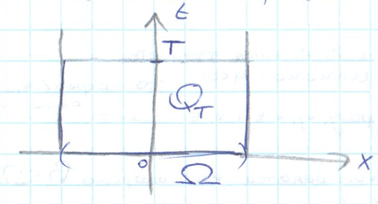
\includegraphics[scale=0.5]{part3.1.png}
\end{center}
% TODO: изображение

\begin{theorem}[Принцип максимума в ограниченной области]

Пусть $u$ - классическое решение уравнения теплопроводности в ограниченной области $\Omega$. Тогда оно достигает максимума на $S_T$ для любого $T$.
\end{theorem}
\begin{proof}
Прежде всего стоит заметить, что максимум достигается, ведь $\overline{Q}_T$ - компакт.

Обозначим точку максимума $u$ через $(t_0, x_0)$. Введем обозначение для оператора теплопроводности:
$$ Lu  = u_t - a^2 \Delta u.$$
Рассмотрим 
$$ v_{\eps} (t,x) = u(t,x) + \eps \abs{x}^2 \quad (\abs{v_{\eps}} > \abs{u})$$
Тогда
$$ L v_{\eps} = \pder[v_{\eps}]{t} - a^2 \Delta v_{\eps} = u_t - a^2 \Delta u - \eps a^2 \underbrace{\Delta \abs{x}^2}_{=2n} = Lu - 2 \eps a^2 n = - 2 \eps a^2 n.$$
Пусть $(t_{\eps}, x_{\eps}) \in \overline{Q}_T$ - точка максимума $v_{\eps}$. Где именно она находится? Возможны три случая:

\begin{enumerate}
\item $(t_{\eps}, x_{\eps}) \in Q_T$ - внутри цилиндра. Так как точка максимума находится в открытом множестве, то в ней все первые производные равны нулю, нас интересует $$v_{\eps, t} = 0.$$
В то же время в точке максимума вторые производные неположительны: $$ v_{\eps, x_i x_i} \leq 0, \quad \forall i \in 1:n $$
Получаем:
$$Lv_{\eps}  = \underbrace {v_{\eps,t}}_{=0} - \underbrace {a^2 \Delta v_{\eps}}_{\leq 0} \geq 0, \quad L v_{\eps} = -2n \eps a^2 < 0$$
Противоречие. Значит, $(t_{\eps}, x_{\eps}) \notin Q_T$.
\item $(t_{\eps}, x_{\eps}) \in \left\{ T \right\} \times \Omega$ - на верхней крышке. По той же причине вторые производные по пространственным координатам неположительны:
$$ v_{\eps, x_i x_i} \leq 0.$$
Максимум достигается на правой границе временного интервала, значит,
$$v_{\eps,t} \geq 0$$
Имеем:
$$Lv_{\eps}  = \underbrace {v_{\eps,t}}_{\geq 0} - \underbrace {a^2 \Delta v_{\eps}}_{\leq 0} \geq 0, \quad L v_{\eps} = -2n \eps a^2 < 0$$
Противоречие. Значит, $(t_{\eps}, x_{\eps}) \notin \left\{ T \right\} \times \Omega$.
\item $(t_{\eps}, v_{\eps}) \in S_T$ - на параболической границе. Единственный оставшийся вариант.
\end{enumerate}
Имеем:
$$ u(t,x) \leq v_{\eps} (t,x) \leq \max_{S_T} v_{\eps} \leq \max_{S_T} u + \eps \underbrace {(\diam \Omega)^2}_{=\const} \xrightarrow[\eps \to 0]{} \max_{S_T} u.$$
Таким образом, максимум $u$ достигается на $S_T$.

\end{proof}

\begin{corollary}[Принцип минимума]
Пусть $u$ - классическое решение уравнения теплопроводности в ограниченной области $\Omega$. Тогда оно достигает минимума на $S_T$ для любого $T$.
\end{corollary}
\begin{proof}
Аналогично, только вместо $u$ рассматриваем $-u$.

\end{proof}

\begin{corollary}[Единственность]
Начально-краевая задача в $\Omega$
\begin{gather*}
	\begin{cases*}
		u_t - a^2 \Delta u = f, \\
		u \Big\rvert_{\partial \Omega} = h, \\
		u(0, x) = g.
	\end{cases*}
\end{gather*}
может иметь не более одного решения.
\end{corollary}
\begin {proof}
Пусть $u_1$ и $u_2$ - решения. Тогда их разность удовлетворяет соответствующему однородному уравнению:
\begin{gather*}
	\begin{cases*}
		L(u_1 - u_2) = 0, \\
		(u_1 - u_2) \Big\rvert_{\partial \Omega} = 0, \\
		(u_1 - u_2) \Big\rvert_{t = 0} = 0.
	\end{cases*}
\end{gather*}
Из однородного уравнения разность наших решений равна нулю на всей границе, а по доказанной теореме максимум и минимум разности достигаются на параболической границе $S_T \subset \real^+ \times \Omega$. Значит,
$$0 = \min (u_1 - u_2) \leq (u_1 - u_2) \leq \max (u_1 - u_2) = 0 \quad \Rightarrow \quad u_1 - u_2 \equiv 0$$

\end{proof}
\begin{corollary}[Поведение решений при $t \to \infty$] Рассмотрим температурное поле в ограниченной области $\Omega$:
\begin{gather*}
	\begin{cases*}
		u_t - a^2 \Delta u = 0, \\
		u \Big\rvert_{\partial \Omega} = 0, \\
		u \Big\rvert_{t = 0} = g.
	\end{cases*}
\end{gather*}
То есть, на стенках поддерживается нулевая температура, в начальное время задано температурное поле $g$, источников и стоков теплоты внутри области нет. Тогда
$$ u(t,x) \xrightarrow[t \to \infty]{} 0$$
равномерно по $x$ и экспоненциально по $t$.
\end{corollary}
\begin{proof}
Будем считать, что $0 \in \Omega$. Рассмотрим
$$ v(t,x) = A e^{-bt} \prod \limits_{i=1}^n \cos C x_i. $$
Так как $\Omega$ - область ограниченная, то она лежит в некотором $n$-мерном кубе. Значит, можно подобрать $C$ так, чтобы каждый из косинусов был положителен. Выбор $C$ зависит только от диаметра $\Omega$. Далее, применим оператор теплопроводности к $v$:
$$ Lv = -b \cdot v(t,x) + n a^2 C^2 \cdot v(t,x) = (na^2C^2 - b^2) \cdot v.$$
Если $b = n a^2 C^2$, то $Lv = 0$. По этой формуле можем подобрать $b$. Теперь выбираем большое $A$ такое, что
$$ v(0,x) = A \prod \limits_{i=1}^n \cos C x_i > \max_{x \in \Omega} |g(x)|.$$

Имеем $$Lv = 0,\quad v(0,x) \geq \abs{g(x)},\quad v \geq 0 .$$ Рассмотрим
$$ w_{\pm} = v \pm u.$$
Тогда:
\begin{gather*}
	Lw_{\pm} = 0, \\
	w_{\pm}\Big\rvert_{\partial \Omega} = v\Big\rvert_{\partial \Omega} \pm u\Big\rvert_{\partial \Omega} \geq 0, \\
	w_{\pm}\Big\rvert_{t=0} = \underbrace {v\Big\rvert_{t=0}}_{\geq \abs{g}} \pm \underbrace{u\Big\rvert_{t=0}}_{=g} \geq 0.
\end{gather*}

Таким образом, $w_{\pm}$ - решения в $\real^n \times \Omega$ и положительны на $S_T$, а по принципу минимума $w_{\pm} > 0$  на $\real^n \times \Omega$. Из определения $w_{\pm}$ 
$$\abs{u(t,x)} \leq v(t,x) = A e^{-bt} \prod \limits_{i=1}^n \cos c x_i \xrightarrow[t \to \infty]{} 0.$$
Выбор констант $A$, $C$ и $b$ зависит только от $\diam \Omega$. Оценивая косинусы единицей, получаем, что
$$ \abs{u(t,x)} \leq A e^{-bt} \xrightarrow[t \to \infty]{} 0$$
равномерно по $x$, экспоненциально по $t$.

\end{proof}


\begin{note} Пусть существует классическое решение $\overline{u}$ задачи
\begin{gather*}
	\begin{cases*}
		\Delta \overline{u} = 0, \\
		\overline{u}\Big\rvert_{\partial \Omega} = h(x).
	\end{cases*}
\end{gather*}
Тогда для решения $u$ задачи 
\begin{gather*}
	\begin{cases*}
		u_t - a^2 \Delta u = 0, \\
		u \Big\rvert_{\partial \Omega} = h(x), \\
		u(0, x) = g(x)
	\end{cases*}
\end{gather*}
верно, что $$u \xrightarrow[t \to \infty]{} \overline{u}$$
равномерно по $x$, экспоненциально по $t$.
\end{note}

\begin{proof}
Рассмотрим $v = u - \overline{u}$. Тогда
\begin{align*}
& Lv = Lu - L\overline{u} = 0, \\
& v\Big\rvert_{\partial \Omega} = h - h = 0, \\
& v\Big\rvert_{t = 0} = g(x) - \overline{u}(x).
\end{align*}
Заметим, что $v$ удовлетворяет условию следствия 3. Значит, $ v \xrightarrow[t \to 0]{} 0$, и $ u \to \overline{u}$.

\end{proof}
% !TEX encoding = UTF-8 Unicode
% лекция 4, 5 апреля 2016
% Принцип максимума для уравнения теплопроводности во всем пространстве для функций, ограниченных в каждой полосе.
% 2 следствия. Фундаментальное решение для уравнения теплопроводности. Теорема интегральная формула для решения 
% задачи Коши для однородного уравнения теплопроводности в пространстве. Свойства решения. Решение задачи Коши для
% неоднородного уравнения теплопроводности в пространстве. Метод Дюамеля.

\section{Принцип максимума для уравнения теплопроводности во всем пространстве}
Поставим задачу Коши для уравнения теплопроводности во всем пространстве:
\begin{align}
    \begin{cases} 
        u_t - a^2 u_x = 0, \\
        u (0, x) = \varphi (x).
    \end{cases}
\label{transcalency}
\end{align}
[рисунок, относится к цилиндрам]
Будем рассматривать решения на бесконечных цилиндрах $u : \real^+ \times \real^n \rightarrow \real,$ считаем, что все производные существуют вплоть до $t = T$, поскольку решение рассматриваем на всем $\real^+ \times \real^n $.Ограничим класс интересующих нас функций, т.е. дополнительно потребуем: $ \forall T > 0 \quad \exists C = C(T) > 0 : |u(t, x)| \leq C(T) \quad \forall t \in [0, T] \quad \forall x \in \real^n$ (в каждой ограниченной полосе решение $u(t, x)$ - ограничено, ясно, что ограниченность зависит от $t$). Тогда имеем теорему в наших условиях:

\begin{theorem}{(Принцип максимума для уравнения тепопроводности \\ в $\real^n$ для функций, ограниченных в каждой полосе).}

Пусть $T > 0$ $$ M_+ = \sup_{\stackrel{x \in \real^n,} {t \in [0, T]}}u(t,x), \quad N_+ = \sup_{x \in \real^n} u(0, x), $$ то $M_+ = N_+$ (супремум по всей полосе есть супремум при $t = 0$)

\begin{note}Очевидно, что $-\infty < N_+ \leq M_+ < +\infty.$ Почему очевидно? Потому что ограничено в полосе.\end{note}
\end{theorem}

\begin{proof}
Рассмотрим произвольное $\eps.$
$$v_\eps(t, x) = u(t, x) - \eps(2na^2t + \abs{x}^2), \qquad Lu = u_t - a^2v$$
$$Lv_\eps = \underbrace{Lu}_{0} - \eps L(2na^2t + \abs{x}^2) = -\eps(2na^2 - 2n\bigtriangleup x^2) = -\eps(2na^2 - 2na^2) = 0,$$
т.~к. $\bigtriangleup \abs{x}^2 = \bigtriangleup(x_1^2 + x_2^2 + \dots + x_n^2) = \sum_{i = 1}^{n} \dfrac{\partial^2 |x|^2}{\partial x_i^2} = 2n$, т.~о. $v_\eps$ --- тоже решение уравнения теплопроводности во всем пространстве.

[picture] Теперь будем рассматривать открытые цилиндры $Q_{T,R} = (O,T)\times B_R(0)$, полоса --- объединение всех таких цилиндров по $R$. По принципу максимума для решения уравнения теплопроводности в ограниченной области (можем применить, т.к. цилиндр компактен) [здесь будет номер теормы вместо огромного названия] максимум и минимум достигаются на параболической границе. Посмотрим на поведение функции на параболической границе.
Нижняя граница:
$$ v_\eps (0,x) = u(0,x) - \eps |x|^2 \leq N_+ \forall x$$
Боковая поверхность:
$$v_\eps(t,x)\Bigl|_{\abs{x} = R} = u(t,x) \Bigl|_{\abs{x} = R} - \eps(2na^2t + R^2) \leq u(t,x)\Bigl|_{\abs{x} = R} - \eps R^2 \leq M_+ - \eps R^2 \leq N_+$$
Подберем $R: \, M_+ - \eps R^2 \leq N_+$ (Почему так можно сделать? Использовали то, что $M_+$ и $N_+$ --- это числа, ни одно из них не бесконечность, $R(\eps)$ можно выразить как ${R(\eps) = \dfrac{\sqrt{M_+ - N_+}}{\eps} \stackrel{\eps \rightarrow 0} \longrightarrow \infty}$).

Т.~о. $ v_\eps (t, x) \leq N_+ \, \forall (t,x) \in {Q_{T,R(\eps)}};$
$(t,x) \in [0,T] \times \real^n$ нужно доказать, что $u(t,x) \leq N_+.$
$$\text{При }\eps \rightarrow 0, \, \text{начиная с какого-то }\eps \, (t,x) \in Q_{T,R} \Rightarrow$$
$$v_\eps(t,x) = u(t,x) - \eps(2na^2t - \abs{x}^2) \leq N_+ \forall \eps \geq \eps_0 \Rightarrow$$
$$u(t,x) \leq N_+ + \eps\underbrace{(2na^2t + |x|^2)}_{const} \stackrel{\eps \rightarrow 0}{\Rightarrow} u(t,x) \leq N_+$$
Т.~о. $M_+ = N_+.$
\end{proof}

\begin{consequence}{(Принцип минимума для уравнения теплопроводности во всем пространстве)}
$$M_- = \inf_{\stackrel{x \in \real^n, \,} {t \in [0, T]}}u(t,x); \qquad N_- = \inf_{x \in \real^n}u(0,x),$$
то $M_-=N_-$ (инфимум по полосе равен инфимуму по нижней границе).
\end{consequence}

\begin{consequence}{(Единственность)}
Рассмотрим задачу Коши для неоднородного уравнения:
\begin{align}
    \begin{cases} 
        u_t - a^2 \bigtriangleup u = q, \\
        u (0, x) = \varphi (x).
    \end{cases}
\label{transcalencynonhom}
\end{align}
Классическое решение для задачи \eqref{transcalencynonhom} --- единственное в классе функций, ограниченных в каждой полосе.
\end{consequence}

\begin{proof}
Пусть $u_1, \, u_2 $ --- два решения. $L$ --- оператор теплопроводности.
$$Lu_1=Lu_2=q \Rightarrow L(u_1 - u_2) = 0;$$
$$u_1\Bigl|_{t=0} = u_2\Bigl|_{t=0}=\varphi(x) \Rightarrow (u_1-u_2)\Bigl|_{t=0}=0,$$
т.~о. $u = u_1 - u_2$ --- решение однородной задачи с нулевыми начальными условиями (в том же классе ограниченных в полосе функций), т.~о. по теореме 3 $\sup u = 0 \, \text{и} \, \inf u = 0 \Rightarrow u \equiv 0 \Rightarrow u_1 = u_2.$
\end{proof}

\begin{note}
Условие ограниченности в каждой полосе необходимо, т.к. если его убрать, решение не будет единственным, будет решение в полосе и еще какое-то быстрорастущее решение, единственности нет. Неединственность относится уже не к теплопроводности, поэтому физики тоже накладывают ограничения, чтобы получать единственное решение, относящееся к теплопроводности.
\end{note}

\section{Фундаментальное решение для уравнения теплопроводности}

Хотим получить решение для системы \eqref{transcalency}. Получим --- фундаментальное решение уравнения теплопроводности (в ходе решения будем накладывать некоторые специфические условия на решение).

Рассмотрим $a = 1$ иначе можно сделать замену $x \rightarrow \dfrac{x}{a}$ (делаем это для упрощения вычислений).

\begin{enumerate}
\item $u(t,x) = \lambda^\alpha u(\lambda t, \lambda^\beta x) \quad \forall \lambda$ (т.~е. хотим частичную линейность решения)

Рассмотрим $\lambda = \dfrac{1} {t}. \, \alpha, \, \beta$ --- неизвестны.
$$u(t,x) = \dfrac{1}{t^\alpha}(1, \dfrac{x}{t^\beta}) \text{. Обозначим } \, u(1,z) = v(z) \Rightarrow u(t,x) = \dfrac{1}{t^\alpha} v(\dfrac{x}{t^\beta}).$$
Посчитаем $Lu = 0$:
$$-\dfrac{\alpha}{t^{\alpha + 1}} v\left( \dfrac{x}{t^\beta}\right) - \dfrac{\beta}{t^{\alpha + \beta + 1}}\nabla v\left( \dfrac{x}{t^\beta}\right)\cdot x - \dfrac{1}{t^\alpha t^{2\beta}}\bigtriangleup v\left( \dfrac{x}{t^\beta}\right) = 0.$$
$$\left(\text{т.к.} \, \dfrac{\partial}{\partial t} \left(v\left( \dfrac{x}{t^\beta}\right)\right) = \sum \dfrac{ \partial v}{\partial x_i}\left(\dfrac{x}{t^\beta}\right) \cdot \dfrac{-\beta x_i}{t^{\beta + 1}} = -\dfrac{\beta}{t^{\beta + 1}}\nabla v\left( \dfrac{x}{t^\beta}\right) \cdot x \right)$$

Сделаем замену $ y = \dfrac{x} {t^\beta}.$
$$ \dfrac{\alpha}{t^{\alpha + 1}} v(y) + \dfrac{\beta}{t^{\alpha + 1}} \nabla v(y) \cdot y + \dfrac{1}{t^\alpha  t^{2\beta}}\bigtriangleup v(y)=0.$$

Пусть $\beta = \dfrac{1}{2}$ и умножаем полученное выражение на $t^{\alpha + 1}:$
$$\alpha v(y) + \dfrac{1}{2} \nabla v(y) \cdot y + \bigtriangleup v(y) = 0.$$

\item $u(t,x) = \tilde{u}(t,|x|)$ --- хотим симметрии относительно 0, т.~о. $v(y) = w(|y|), |y| = r.$ Тогда получим:
$$ \alpha w(r) + \dfrac{1}{2} w'(r) \cdot r + w''(r) + \dfrac{n}{r}w'(r) = 0;$$
$$\text{т.~к.} \quad \bigtriangleup v(y) = \dfrac{\partial^2v}{\partial y_1^2} + \dots + \dfrac{\partial^2v}{\partial y_n^2};$$
$$\dfrac{\partial w}{\partial y_i} = w' \dfrac{\partial |y|}{\partial y_i} = w' \dfrac{y_i}{r} \Rightarrow 
\dfrac{\partial^2 w}{\partial y_i^2} = w''\dfrac{y_i^2}{r^2} + w'\left(\dfrac{1}{r} - \dfrac{y_i^2}{r^2}\right) \Rightarrow$$
$$\bigtriangleup w(r) = \dfrac{w''}{r^2}\sum y_i^2 + \dfrac{w'}{r}\sum (1 - \dfrac{y_i^2}{r^2}) = w'' + \dfrac{w'n}{r}.$$

Пусть $\alpha = \dfrac{n}{2}.$
$$\dfrac{n}{2}w(r) + \dfrac{1}{2}w'(r) \cdot r + w''(r) + \dfrac{n-1}{r}w'(r) = 0 \Rightarrow$$$$ \dfrac{1}{2}\left(r^nw\right)' + \left(r^{n-1}w'\right)' = 0 \Rightarrow \dfrac{1}{2}\left(r^nw\right)+ \left(r^{n-1}w'\right) = \gamma.$$

\item $r^aw_n' + r^bw \rightarrow 0 \, \text{при} \, n \rightarrow \infty$ --- хотим, чтобы это выполнялось, такое возможно только при $\gamma = 0,$ т.~о.
$$r^{n-1}w_r' + \dfrac{1}{2}r^nw = 0 \Rightarrow w_r' + \dfrac{r}{2}w = 0 \Rightarrow$$
$$\dfrac{dw}{w} = -\dfrac{r}{2}dr \Rightarrow w = be^{-\dfrac{r^2}{4}},$$
$$\text{т.~о.} \, u(t,x) = \dfrac{1}{\sqrt{t^n}}u\left(1, \dfrac{x}{\sqrt{t}}\right) = \dfrac{1}{\sqrt{t^n}}w\left(\dfrac{x}{\sqrt{t}}\right) = \dfrac{b}{\sqrt{t^n}}e^{-\dfrac{|x|^2}{4t}}.$$

Получили однопараметрическое семейство решений.
\begin{note}Если зафиксируем $t$, то полученное выражение --- гауссова функция(нормальное распределение)[рисунок], чем $t$ меньше, тем выше "пика" на графике, соответственно, чем больше, тем более сглаженным будет график.
\end{note}
Теперь определенным образом выберем константу, пусть $b\,:\,b>0; \, \int\limits_{\real^n} u(t,x)dx = 1.$

\begin{note}
Нужно уметь вычислять $b$.
\end{note}

$$b = \dfrac{1}{(4\pi)^{n/2}} \Rightarrow$$$$ u(t,x) = \dfrac{1}{(4\pi t)^{n/2}} \exp\left(-\dfrac{|x|^2}{4t}\right) = \Phi(t,x) \,\text{--- фундаментальное решение уравнения теплопроводности.}$$
\begin{note}
Что если $a \not= 1$?
\end{note}
\end{enumerate}

\begin{theorem}(Интегральная формула для решения задачи Коши)
$ \varphi\in C_b(\real^n)$ --- ограниченная и непрерывная(начальное распределение). Тогда
$$u(t,x) = \int\limits_{\real^n}\Phi(t, x-y)\varphi(y)dy (= \left(\Phi(t,\cdot)*\varphi\right)(x) \text{ --- свертка.})$$
\begin{enumerate}
\item $u \in C^\infty\left(\left(0, +\infty\right)\times \real^n\right);$
\item $ u_t - \bigtriangleup u = 0$ --- т.~е. решение уравнения теплороводности;
\item $\lim\limits_{(t,\,y) \rightarrow (0,\,x)}u(t,x) = \varphi (x).$
\end{enumerate}
\end{theorem}
\begin{note}{Физический смысл фундаментального решения.} %%%слишком много сказано, нужно ли писать, вроде смысла нет.
$\Phi$ - распределение температуры от единичного источника (источник с температурой единица), сосредоточенного в одной точке. 
\end{note}
\begin{proof}
\begin{enumerate}
\item $\Phi \in  C^\infty\left(\left(0, +\infty\right)\times \real^n\right)$ --- очевидно.
$$u_t = \int\limits_{\real^n} \Phi_t(t,x-y)\varphi(y)dy, \qquad u_{x_i} = \int\limits_{\real^n} \Phi_{x_i}(t, x-y)\varphi(y)dy$$

Очевидно, $u \in C^\infty.$
\item $Lu = u_t - \bigtriangleup u = \int\limits_{\real^n} \underbrace{(\Phi_t - \bigtriangleup \Phi)(t, x-y)}_{0}\varphi(y) dy = 0.$
\item Пусть $x_0 \in \real^n.$
$$|u(t,x) - \varphi(x_0)| = \Bigl|\int\limits_{\real^n}{\Phi(t,x-y)\varphi(y)dy} - \varphi(x_0)\Bigl| = \Bigl|\int\limits_{\real^n}\Phi(t,x-y)\varphi(y)dy - \varphi(x_0)\int\limits_{\real^n}\Phi(t,x-y)dy\Bigl|=$$
$$=\Bigl|\int\limits_{\real^n}\Phi(t,x-y)(\varphi(y) - \varphi(x_0))dy\Bigl| \leq \int\limits_{\real^n}\Phi(t,x-y)\bigl|\varphi(y) - \varphi(x_0)\bigl|dy = $$
$$= \underbrace{\int\limits_{B_\delta(x_0)}\Phi(t,x-y)\bigl|\varphi(y) - \varphi(x_0)\bigl|dy}_{I_\delta} + \underbrace{\int\limits_{\real^n \setminus B_\delta(x_0)}\Phi(t,x-y)\bigl|\varphi(y) - \varphi(x_0)\bigl|dy}_{J_\delta}.$$

Пусть $\eps > 0.$ Выберем такое $\delta,$ что $\bigl|\varphi(y) - \varphi(x_0)\bigl|<\dfrac{\eps}{2}$ при $y \in B_\delta(x_0)$ (Такое $\delta \, \exists,$ т.~к. $\varphi$ --- непрерывна).

Тогда $I_\delta \leq \dfrac{\eps}{2}, \, \text{т.к.} \int\limits_{\real^n}\Phi = 1.$

Пусть $|x - x_0| < \dfrac{\delta}{2}, \, y \notin B_\delta(x_0) \Rightarrow |x - y| \geq \dfrac{1}{2}|x_0 - y|.$
$$J_\delta \leq 2||\varphi||_\infty \cdot \int\limits_{\real^n \setminus B_\delta(x_0)} \Phi(t,x-y)dy = 2||\varphi||_\infty \dfrac{1}{(4\pi t)^{n / 2}} \int\limits_{B_{\delta}^c} e^{-\dfrac{|x-y|^2}{4t}}dy \leq $$$$\leq 2||\varphi||_\infty \dfrac{1}{(4\pi t)^{n / 2}} \int\limits_{B_{\delta}^c} e^{-\dfrac{|x_0-y|^2}{16t}}dy \leq \dfrac{C}{(4\pi t)^{n / 2}} \int\limits_\delta^{+\infty} e^{-\dfrac{\rho^2}{16t}}\rho^{n-1}d\rho =  $$$$ = C\int\limits_{\delta / \sqrt{t}}^{+\infty} e^{-\dfrac{\rho^2}{16t}}\rho^{n-1}d\rho \stackrel{t\rightarrow 0}{\longrightarrow} 0$$
$$\delta: \, t < \dfrac{\delta}{2}, \, J_\delta \leq \dfrac{\eps}{2}, \Rightarrow I = I_\delta + J_\delta \leq \eps, \, |x-x_0| < \dfrac{\delta}{2}, \, 0<t<\dfrac{\delta}{2} \Rightarrow $$$$ |u(t,x) - \varphi(x_0)|<\eps$$
\end{enumerate}
\end{proof}

\section{Решение задачи Коши для неоднородного уравнения теплопроводности в пространстве. Метод Дюамеля}
\begin{align}
    \begin{cases} 
        u_t - \bigtriangleup u = f, \\
        u (0, x) = \varphi (x).
    \end{cases}
\label{transcalencynonhom2}
\end{align}
$t \in \real^+,\, x \in \real^n, f=f(t,x)$

\begin{note}

Достаточно решать для случая $\varphi = 0, \, f \not= 0 \, \text{и} \, \varphi \not=, \, f = 0,$ т. е. пусть $u_1, \, u_2 :$
\begin{equation*}
\begin{cases} 
        Lu_1 = f, \\
        u_1\Bigl|_{t=0} = 0.
    \end{cases}
    \qquad
    \begin{cases} 
        Lu_2 = 0, \\
        u_2\Bigl|_{t=0} = \varphi (x).
    \end{cases}
\end{equation*}
Тогда $u = u_1+u_2:$
\begin{align}
\begin{cases} 
        Lu = f, \\
        u\Bigl|_{t=0} = \varphi (x).
    \end{cases}
    \end{align}
\end{note}

{\itshape Принцип Дюамеля.} Пусть $\varphi = 0$
\begin{equation*}
v(t,x,s) : \quad
    \begin{cases} 
        v_t - \bigtriangleup v = 0, \\
        v\Bigl|_{t=s} = f(s, \,).
    \end{cases}
\end{equation*}
$$u(t,x) = \int\limits_0^tv(t,x,s)ds = \int\limits_0^t ds \int\limits_{\real^n}\Phi(t-s, x-y)f(s,y)dy.$$

\begin{theorem}
Пусть $ u(t,x) = \int\limits_0^t ds \int\limits_{\real^n}\Phi(t-s, x-y)f(s,y)dy,$ тогда при $f\in C_x^2, \, C_t^1, f $ --- финитная $\in C_0^\infty( (0,+\infty) \times \real^n),$
\begin{enumerate}
\item $u \in C_t^1, \, u \in C_x^2;$
\item $u_t(t,x) - \bigtriangleup u(t,x) = f, \, u(0,x) = 0;$
\item $\lim u(t,x) = 0$ при $(t,x) \rightarrow (0,x_0) \forall x_0 \in \real^n.$
\end{enumerate}
\end{theorem}

\begin{proof}

$$u(t,x) = \int\limits_0^t ds \int\limits_{\real^n} \Phi(s,y)f(t-s, x-y)dy \, \text{--- свертка},$$ т.к. $f\in C_x^2, \, C_t^1, f $ --- финитная и $\Phi(s,y)$ гладкая в окрестности $s = t >0:$
$$\dfrac{\partial^2u}{\partial x_i^2} = \int\limits_0^t ds \int\limits_{\real^n} \Phi(s,y)f_{x_i x_i}(t-s, x-y)dy;$$
$$u_t = \int\limits_{\real^n} \Phi(t,y)f(0,x-y)dy + \int\limits_0^t ds\int\limits_{\real^n} \Phi(s,y)f_t(t-s, x-y)dy,$$ т.е. $u \in C_t^1, \, u \in C_x^2.$

$$u_t - \bigtriangleup u = \int\limits_{\real^n} \Phi(t,y)f(0,x-y)dy + \int\limits_0^t ds\int\limits_{\real^n} \Phi(s,y)f_t(t-s, x-y)dy-$$$$ - \int\limits_0^t ds \int\limits_{\real^n}dy\underbrace{\sum \Phi(s,y)f_{x_i x_i}(t-s, x-y)}_{\Phi(s,y)\bigtriangleup f(t-s, x-y)} = $$
$$= \int\limits_{\real^n} \Phi(t,y)f(0,x-y)dy + \int\limits_0^t ds \int\limits_{\real^n}dy \Phi(s,y)(-\dfrac{\partial}{\partial s} - \bigtriangleup y) = $$ $$= \underbrace{ \int\limits_0^\eps ds \int\limits_{\real^n}\Phi(s,y)\left(\left(-\dfrac{\partial}{\partial s} - \bigtriangleup y\right)f(t-s, x-y)\right)dy}_{I_\eps} + \underbrace{\int\limits_{\real^n} \Phi(t,y)f(0,x-y)dy}_{k} + $$
$$+ \underbrace{\int\limits_\eps^t ds \int\limits_{\real^n} \Phi(s,y)\left(\left(-\dfrac{\partial}{\partial s} - \bigtriangleup y\right)f(t-s, x-y)\right)dy}_{J_\eps}.$$
$$\abs{I_\eps} \leq \left(||f_t||_\infty + ||\bigtriangleup_x f||_\infty\right)\int\limits_0^\eps ds \int\limits_{\real^n}\Phi(s,y)dy = C\eps.$$
$$J_\eps = \int\limits_\eps^t ds \underbrace{\int\limits_{\real^n}\left(\left(\dfrac{\partial}{\partial s} - \bigtriangleup y\right)\Phi(s,y)\right)f(t-s, x-y)dy}_{0, \, \text{т.к.} \, \Phi \, \text{--- решение однородного уравнения}} + \int\limits_{\real^n} \Phi(\eps, y)f(t-\eps, x-y)dy - $$ $$-\underbrace{\int\limits_{\real^n} \Phi(t,y)f(0,x-y)dy}_{\text{это} \, k}.$$
При $\eps \rightarrow 0:$
$$u_t - \bigtriangleup u = \lim_{\eps \rightarrow 0} \int\limits_{\real^n}\Phi(\eps, y)f(t-\eps, x-y)dy = \lim_{\eps \rightarrow 0} \int\limits_{\real^n}\Phi(\eps, x-y)f(t-\eps, y)dy = f(t,x) \Rightarrow$$ $\Rightarrow u$ --- решение.

$$\abs{u(t,x)} \leq \int\limits_0^t ds \int\limits_{\real^n}\Phi(s,y)\underbrace{\abs{f(t-s, x-y)}}_{\leq C, \, \text{т.к. финитная}}dy \leq C\int\limits_0^t ds \int\limits_{\real^n}\Phi(s,y)dy = Ct \stackrel{t \rightarrow 0} \longrightarrow 0. $$
\end{proof}





% !TEX encoding = UTF-8 Unicode
% лекции 9-10, 12 марта 2016
% вопросы 18-20 
% 18. Пространство основных функций и пространство обобщенных функций (распределений). Примеры обобщенных функций. Дифференцирование обобщенных функций. Обобщенные и классические производные.
% 19. Фундаментальное решение уравнения Лапласа, его физический смысл.
% 20. Представление (частного) решения уравнения Пуассона в пространстве при помощи фундаментального решения.

\subsection{Основы теории обобщенных функций}
Как и раньше, $\Omega \subset \real^n$ --- область.
\begin{definition}
Множество $ \beauD(\Omega) = C_0^\infty(\Omega)$ называется пространством основных функций (пробных функций).
\end{definition}
\begin{definition}
Последовательность функций $\{u_k\} \subset C_0^\infty(\Omega)$ сходится к основной функции $u \in C_0^\infty(\Omega)$, если 
\begin{enumerate}
\item все функции последовательности имеют носитель в одном компакте: $$\exists K \ssubset \Omega: \quad \supp u_k \subset K,$$
\item все функции последовательности и все их производные сходятся к $u$ и её производным равномерно $$u_k \rightrightarrows u, \quad D^\alpha u_k \rightrightarrows D^\alpha u \quad \forall \alpha,$$ где $\alpha$ --- мультииндекс: $$\alpha = (\alpha_1, \ldots, \alpha_n), \, \alpha_i \in \mathds{N},$$ $$\abs{\alpha} = \sum\limits_{i=1}^{n}\alpha_i,$$
$$D^\alpha u = \dfrac{\partial^{\abs{\alpha}}u}{\partial x_1^{\alpha_1}\ldots\partial x_n^{\alpha_n}}.$$
\end{enumerate}
\end{definition}

\begin{example}Пусть $u_0 \in C_0^\infty(\real)$ и $u_k = \dfrac{1}{k}u_0$, тогда $u_k \conv*{\beauD(\real)}{} 0$.
\end{example}

\begin{example}Пусть $u_0 \in C_0^\infty(\real)$ и $u_k(x) = \dfrac{1}{k}u_0(x - k)$. Тогда
\begin{gather*}
	u_k \to 0, \\
	u_k \rightrightarrows 0, \\
	D^\alpha u_k \rightrightarrows 0 \quad \forall \alpha
\end{gather*}
но $u_k$ не живут на одном компакте, так что $$ u_k \centernot {\conv*{\beauD(\real)}{}} 0.$$

Таким образом, сходимость основных функций сильнее, чем равномерная или поточечная.
\end{example}

\begin{note} Заданная нами на $\beauD$ топология не порождается никакой метрикой. 
\end{note}

\begin{definition}
Пространством обобщенных функций $\beauD'(\Omega)$ называется пространство линейных непрерывных функционалов на пространстве $\beauD(\Omega)$. Через $\action{u,f}$ обозначается действие обобщенной функции $f$ на основную функцию $u$. Обобщенные функции также называют распределениями.
\end{definition}

\begin{note} Таким образом, обобщённая функция это не функция, а функционал.
\end{note}

\begin{note} Пусть $\left\{ u_k \right\} \subset \beauD(\Omega)$. Непрерывность обобщённой функции $f$ означает, что
$$ u_k \conv* {\beauD(\Omega)} {} u \quad \Rightarrow \quad \action{u_k, f} \longrightarrow \action{u, f}.$$
\end{note}

\begin{example} Любая функция $v \in L_{loc}^1 (\Omega)$ канонически порождает обобщённую функцию $\widehat{v}$:
$$ \action{u, \widehat{v}} = \int \limits_\Omega u(x) v(x) \, dx.$$
Интеграл имеет смысл, так как на самом деле мы интегрируем по $\supp u$. Линейность $\widehat{v}$ очевидна, покажем непрерыность. Пусть $\left\{ u_k \right\} \subset \beauD(\Omega)$ и $ u_k \conv*{\beauD(\Omega)}{} u$, тогда
$$ \action{u_k, \widehat{v}} = \int \limits_\Omega u_k v = \int \limits_K u_k v \longrightarrow \int \limits_K uv = \int \limits_\Omega uv = \action{u, \widehat{v}}.$$
Таким образом, можно отождествлять $v = \widehat{v}$ и говорить, что $L_{loc}^1(\Omega) \subset \beauD' (\Omega)$, хоть эти пространства и имеют разную природу.
\end{example}

\begin{example}Конечная положительная борелевская мера $\mu$ порождает обобщённую функцию $\widehat{\mu}$:
$$\action{u, \widehat{\mu}} = \int \limits_\Omega u \, d\mu.$$
Линейность очевидна, непрерывность вытекает из непрерывности интеграла. Таким образом, конечные положительные борелевские меры --- тоже обобщённые функции.
\end{example}

\begin{example}Рассмотрим так называемую дельта-фунцию Дирака $\delta = \delta_0 = \delta(x)$:
$$ \action{u, \delta} = u(0).$$
Также для $x \in \Omega$ можно определить $\delta_{x_0} = \delta (x - x_0)$:
$$\action{u, \delta_{x_0}} = u(x_0).$$
Линейность и непрерывность очевидны. Значит, дельта-функция является обобщённой функцией.
\end{example}

\begin{note}Дельта-функция не порождается никакой функцией из $L_{loc}^1(\Omega)$.
\end{note}
\begin{proof}
Пусть $f \in L_{loc}^1(\Omega)$ такая, что
$$ \action{u, \delta} = \action{u, f} = \int \limits_\Omega fu  = u(0) \quad \forall u \in C_0^{\infty}(\Omega)$$
Рассмотрим такие $u$, у которых $0$ не лежит в носителе. Для них верно
$$\action{u, f} = \int \limits_\Omega fu = 0.$$
По основной лемме вариационного исчисления $f = 0$ почти всюду на $\Omega \setminus \{0\}$. Множество $\{0\}$ имеет меру нуль, значит, $f = 0$ почти всюду на $\Omega$. Подставив в интеграл, получим
$$ u(0) = 0 \quad \forall u \in C_0^{\infty},$$
что невозможно.

\end{proof}

На обобщённых функциях можно определить операции:

\begin{enumerate}
\item Сложение, умножение на скаляр. Пусть $v_1, \, v_2 \in \beauD'(\Omega)$, $\lambda_1,\,\lambda_2 \in \real$, тогда
$$\action{u, \lambda_1v_1 + \lambda_2v_2} = \lambda_1\action{u, v_1} + \lambda_2\action{u, v_2}.$$
\item Умножение на функцию из $C^\infty$. Пусть $\varphi \in C^\infty(\Omega)$, $v\in \beauD'(\Omega)$, $u\in \beauD(\Omega)$, тогда
$$\action{u, \varphi v} = \action{\varphi u, v}.$$
Определение корректно, так как $\varphi u \in C_0^\infty$.
\item Дифференцирование. Пусть $\alpha$ --- мультииндекс, $v\in\beauD'(\Omega)$, $u \in \beauD(\Omega)$. Тогда
$$\action{u, D^\alpha v} = (-1)^{\abs{\alpha}}\action{D^\alpha u, v}.$$
Проверим, что $D^\alpha v\in \beauD'(\Omega)$. Линейность очевидна. Пусть $u_k \conv* {\beauD(\Omega)}{} u$, тогда
$$\action{u_k, D^\alpha v} = (-1)^{\abs{\alpha}} \action{D^\alpha u_k, v} \longrightarrow (-1)^{\abs{\alpha}} \action{D^\alpha u, v} = \action{u, D^\alpha v},$$
по свойствам сходящихся в $\beauD(\Omega)$ последовательностей.
\end{enumerate}

\begin{example}
Пусть $v \in C^1(\Omega) \subset L_{loc}^1(\Omega)$. Тогда $v$ --- обобщенная с точностью до отождествления. Рассмотрим обобщённую функцию $v_{x_i}$:
$$\action{u, v_{x_i}} = - \action{u_{x_i}, v }= - \int \limits_\Omega u_{x_i} v \, dx = \int \limits_\Omega u v_{x_i} \, dx - \underbrace{\int \limits_{\partial \Omega'} u v \nu_i \, d\sigma}_{=0} = \action{u, v_{x_i}},$$
где $\partial \Omega'$ --- гладкая граница некоего множества, лежащего в $\Omega$ и окружающего носитель функции $u$. Здесь мы воспользовались формулой интегрирования по частям для многомерного случая.

\begin{reminder}[Интегрирование по частям (многомерный случай)]
$$\int \limits_{\Omega} u v_{x_i} \,dx = \int \limits_{\partial\Omega} uvn_{i} \,d\sigma - \int \limits_{\Omega} u_{x_i} v \, dx,$$
где $n_{i}$ --- $i$-ая компонента вектора внешней нормали к $\partial\Omega$.
\end{reminder}

Таким образом, если $v$ непрерывно дифференцируема, то обобщённая производная совпадает с классической.
\end{example}

\begin{exercise} Пусть $\Omega = \real$. Рассмотрим обобщённую производную дельта-функции:
$$\action{u, \delta'} = -\action{u, \delta} = -u'(0).$$
Доказать, что ей не соответствуют ни одна функция и ни одна мера.
\end{exercise}

\begin{example}Пусть $\Omega =\real.$ Рассмотрим функцию Хевисайда:
\begin{equation*}
h(x) = \quad
    \begin{cases} 
        1, \, x\geq0\\
        0,\, x < 0.
    \end{cases}
\end{equation*}
Найдём её обобщённую производную:

$$\action{u, h'}= -\action{u',h} = -\int\limits_{-\infty}^{+\infty}u'h = -\int\limits_0^{+\infty}u' = \underbrace{-u\Bigl|_0^{+\infty}}_{\text{финитная}} = 0+u(0)=\action{u,\delta}.$$
Таким образом, $h' = \delta$ в смысле обобщённых функций. В классическом смысле в нуле производной не существует.
\end{example}

\begin{exercise}
Канторова лестница п.в. имеет нулевую производную в классическом смысле. Доказать, что её обобщенная производная $\not\equiv0$  и является мерой, сосредоточенной на канторовом множестве.
\end{exercise}

\subsection{Фундаментальное решение уравнения Лапласа}
Будем рассматривать уравнения Лапласа \eqref{Laplace} и Пуассона \eqref{Poisson} в смысле обобщенных функций.

Пусть $\Omega = \real^n$, $u$ - обобщённая функция. В случае электростатической системы из одного заряда имеем уравнение Пуассона:
\begin{equation}
	-\Delta u = \delta.
\label{comLaplace}
\end{equation}

Нам понадобятся формулы Грина (следуют из формулы интегрирования по частям):
\begin{enumerate}
\item $\displaystyle \int \limits_\Omega v \Delta u = \sum \limits_{i = 1}^{n} \int \limits_\Omega v u_{x_i x_i} = \sum \limits_{i = 1}^{n} \left( - \int \limits_\Omega v_{x_i} u_{x_i} \, dx + \int \limits_{\partial \Omega} v u_{x_i} \nu_i \, d\sigma \right) = - \int \limits_\Omega \nabla u \cdot \nabla v \, dx + \int \limits_{\partial \Omega} v \dfrac{\partial u}{\partial \nu} \, d\sigma.$
\item $\displaystyle \int \limits_{\Omega} \left( u \Delta v - v \Delta u \right) \, dx = \int \limits_{\partial \Omega} \left( u \dfrac{\partial v}{\partial \nu} - v \dfrac{\partial u}{\partial \nu} \right) \, d\sigma.$
\end{enumerate}
Ещё нам понадобятся формулы объёма шара и площади сферы:
$$ |B_1(0)| = \frac{\sqrt{\pi^n}}{\Gamma(\frac {n} {2} + 1)} = \omega_n, \quad  |B_r(0)| = r^n \omega_n, \quad | \partial B_r(0) | = n \omega_n r^{n-1}$$

Будем искать решение \eqref{comLaplace} в смысле обобщенных функций в виде:
$$u(x) = \dfrac{c_n}{\abs{x}^{n-2}}.$$
Пусть $\varphi \in C_0^\infty\left(\real^n\right)$. Посчитаем обобщённый лапласиан от $u$:
\begin{align*}
\action{\varphi, -\Delta u} &= - \action{\Delta \varphi, u} = - \int \limits_{\real^n} \Delta \varphi u \, dx = -c_n \int \limits_{\real^n} \Delta \varphi \dfrac{1}{|x|^{n-2}} \, dx \stackrel{\text{(а)}} {=} - c_n \lim_{\eps \to 0} \int \limits_{B^c_\eps (0)} \Delta \varphi \frac {1} {|x|^{n-2}} \, dx\\
&\stackrel{\text{(б)}} {=} -c_n \lim_{\eps \to 0} \left( \int \limits_{B^c_{\eps}(0)} \varphi \Delta \dfrac{1}{|x|^{n-2}} \, dx + \int \limits_{\partial B_\eps(0)} \left( \dfrac{1}{|x|^{n-2}} \dfrac{\partial \varphi}{\partial\nu} - \varphi \dfrac{\partial}{\partial\nu} \left( \dfrac{1}{|x|^{n-2}} \right) \right) \, d\sigma \right) \\
&\stackrel{\text{(в)}} {=} -c_n \lim_{\eps \to 0} \int \limits_{\partial B_\eps(0)} \left( \dfrac{1}{|x|^{n-2}} \pder[\varphi]{\nu} - \varphi \pder{\nu} \left( \dfrac{1}{|x|^{n-2}} \right) \right) \, d\sigma \\
&= -c_n \lim_{\eps \to 0} \dfrac{1}{\eps^{n-2}} \int \limits_{\partial B_\eps(0)} \pder[\varphi]{\nu} \, d\sigma - \int \limits_{\partial B_\eps(0)} \varphi \pder{\nu} \left( \dfrac{1}{|x|^{n-2}} \right) \, d\sigma \\
&\stackrel{\text{(г)}} {=} c_n \lim_{\eps \to 0} \int \limits_{\partial B_\eps(0)} \varphi \pder{\nu} \left( \dfrac{1}{|x|^{n-2}} \right) \, d\sigma \stackrel{\text{(д)}} {=} c_n\lim_{\eps \to 0} \int \limits_{\partial B_\eps(0)} - \varphi \pder{r} \left( \dfrac{1}{r^{n-2}} \right) \, d\sigma \\
&= c_n \lim_{\eps \to 0} \int \limits_{\partial B_\eps(0)} \varphi \frac{n-2} {|x|^{n-1}} \, d\sigma =  c_n(n-2) \lim_{\eps \to 0} \dfrac{1}{\eps^{n-1}} \int \limits_{\partial B_\eps(0)} \varphi \, d\sigma \\
&\stackrel{\text{(е)}} = c_n n(n-2) \omega_n \lim_{\eps \to 0} \dfrac{1}{| \partial B_\eps(0) |} \int \limits_{\partial B_\eps(0)}\varphi \, d\sigma = c_n n(n-2) \omega_n \lim_{\eps \to 0} \fint \limits_{\partial B_\eps(0)} \varphi \, d\sigma \\
&= c_n n(n-2) \omega_n \varphi(0) = c_n n(n-2) \omega_n \action{\varphi, \delta}.
\end{align*}
Поясним вычисления:
\begin{description}
\item [(а)] исключили особенность в нуле
\item [(б)] воспользовались 2 формулой Грина
\item [(в)] воспользовались тем, что $\Delta\dfrac{1}{\abs{x}^{n-2}} = 0$, остаётся как упражнение
\item [(г)] воспользовались тем, что $$ \Bigg\lvert \int\limits_{\partial B_\eps(0)}\dfrac{\partial\varphi}{\partial\nu} \, d\sigma \Bigg\rvert \leq C\abs{\partial B_\eps(0)} =C\eps^{n-1}, \quad 
 \dfrac{1}{\eps^{n-2}}C\eps^{n-1} = C\eps \conv* {\eps \to 0} {} 0 $$
\item [(д)] воспользовались тем, что $|x| = r$ и вектор нормали к шару это радиальное направление
\item [(е)] домножили и поделили на площадь сферы радиусом $\eps$: $$|\partial B_\eps(0)| = n \omega_n \eps^{n-1}$$
\end{description}

Итого, при $c_n = \dfrac{1}{n(n-2) \omega_n}$ имеем
$$\action{\varphi, -\Delta u} = \action{\varphi, \delta} = \varphi(0) \quad \Rightarrow \quad -\Delta u = \delta.$$
Значит, $$u(x) = \dfrac{1}{n(n-2) \omega_n}\dfrac{1}{\abs{x}^{n-2}}$$ --- обобщённое решение уравнения Лапласа \eqref{comLaplace} в $\real^n$  при $n>2$.

\begin{note}При $n=3$ получим знакомую из школы формулу для потенциала единичного заряда в $\real^3$:
$$c_3 = \dfrac{1}{4\pi}, \quad u(x) = \dfrac{1}{4\pi}\dfrac{1}{\abs{x}}.$$
\end{note}

\begin{exercise}
Проверить, что $$u(x)=\dfrac{1}{2\pi}\ln\dfrac{1}{\abs{x}}$$ удовлетворяет уравнению Лапласа \eqref{comLaplace} в $\real^2$ в обобщенном смысле.
\end{exercise}

\begin{definition}
Фундаментальным решением уравнения Лапласа называется функция
\begin{equation}
\Phi(x) = 
\begin{cases}
-\dfrac{1}{2\pi}\ln\abs{x},\quad n=2,\\
\dfrac{1}{n(n-2)w_n}\dfrac{1}{\abs{x}^{n-2}},\quad n>2.
\end{cases}
\end{equation}
Для неё верно, что
\begin{align*}
& - \Delta\Phi = \delta \text{ в } \beauD'(\real^n), \\
& - \Delta\Phi = 0 \text{ в классическом смысле в } \real^n\setminus\{0\}.
\end{align*}

\end{definition}

\subsection{Представление частного решения уравнения Пуассона в пространстве при помощи фундаментального решения}

\begin{note} [Вывод 3 формулы Грина] Пусть $\Omega\subset\real^n$ --- ограниченная область с гладкой границей, и $0 \in \Omega$. Тогда по 2 формуле Грина:
\begin{align*}
\int \limits_{B^c_\eps(0)} \left( \underbrace{u\Delta\Phi}_{0} - \Phi\Delta u \right) \, dx &= \int \limits_{B^c_\eps(0)} - \Phi \Delta u \, dx = \int \limits_{\partial B^c_\eps(0)} \left( u \dfrac{\partial\Phi}{\partial\nu} - \Phi\dfrac{\partial u}{\partial\nu} \right) \,d\sigma \\
&= \int \limits_{\partial \Omega} \left( u \dfrac{\partial\Phi}{\partial\nu} - \Phi\dfrac{\partial u}{\partial\nu} \right) \,d\sigma + \int\limits_{\partial B_\eps(0)} \left( u \dfrac{\partial\Phi}{\partial\nu} - \Phi\dfrac{\partial u}{\partial\nu} \right) \,d\sigma
\end{align*}
Устремим $\eps$ к нулю:
$$ \int \limits_\Omega - \Phi \Delta u \, dx = \int \limits_{\partial \Omega} \left( u \dfrac{\partial\Phi}{\partial\nu} - \Phi\dfrac{\partial u}{\partial\nu} \right) \,d\sigma + u(0).$$
Перенесём всё в произвольную точку $x_0\in\Omega$:
$$ \int \limits_\Omega - \Phi (x- x_0) \Delta u \, dx = \int \limits_{\partial \Omega} \left( u \dfrac{\partial\Phi}{\partial\nu} (x-x_0) - \Phi (x - x_0) \dfrac{\partial u}{\partial\nu} \right) \,d\sigma + u(x_0).$$
Значит,
$$ u(x_0) = \int \limits_{\partial \Omega} \left( \Phi (x - x_0) \dfrac{\partial u}{\partial\nu} - u \dfrac{\partial\Phi}{\partial\nu} (x-x_0) \right) \,d\sigma - \int \limits_\Omega \Phi (x- x_0) \Delta u \, dx.$$
Получили 3 формулу Грина.
\end{note}

На данный момент мы знаем, что решением уравнения
$$-\Delta u =\delta_{x_0}$$ является функция $$ u=\Phi(x-x_0).$$ Это решение не является единственным: к нему можно добавить любую гармоническую функцию $v$, результат тоже будет решением.

Пусть есть уравнение
$$ - \Delta u = \alpha_1 \delta_{x_1} + \alpha_2 \delta_{x_2},$$
тогда его решением будет
$$ u = \alpha_1 \Phi (x - x_1) + \alpha_2 \Phi (x - x_2).$$
В случае конечной суммы имеем
$$ - \Delta u = \sum_{k = 1}^n \alpha_k \delta_{x_k}, \quad u = \sum_{k=1}^n \alpha_k \Phi (x - x_k).$$
Для произвольной функции интуитивно можно написать
$$-\Delta u = f, \quad u = \int \limits_{\real^n} \Phi(x-y) f(y) \, dy = \Phi*f.$$
Докажем, что при некоторых дополнительных условиях это действительно так.
\begin{theorem}
Пусть $f\in C_0^2(\real^n)$. Тогда
$$ u(x) = \int\limits_{\real^n} \Phi(x-y)f(y)dy$$ будет классическим решением уравнения Пуассона в $\real^n$. 
\begin{note} Классическое решение всегда является обобщенным, так как классические производные равны обобщенным.
\end{note}
\end{theorem}
\begin{proof} Поменяем переменные:
$$u(x) = \int\limits_{\real^n}\Phi(y)f(x-y)dy$$
и продифференцируем $u$ по $x$. Производная проносится под знак интеграла:
$$u_{x_ix_i}=\int\limits_{\real^n}\Phi(y)f_{x_ix_i}(x-y)dy.$$
Тем самым доказана гладкость.

Если 2 классические функции равны в обобщенном смысле, то они просто равны. Докажем, что $u$ --- обобщённое решение уравнения Пуассона.

Пусть $\varphi\in C_0^\infty(\real^n)$, тогда
\begin{align*}
\action{\varphi, -\Delta u} &= \int \limits_{\real^n} \varphi(x)(-\Delta u(x)) \, dx = \int \limits_{\real^n}\varphi(x) \, dx \int \limits_{\real^n} \Phi(y)(-\Delta f(x-y)) \, dy \\
&= \int \limits_{\real^n} \Phi(y) \, dy \int \limits_{\real^n} (-\Delta\varphi(x)) f(\underbrace{x-y}_z) \, dx = \int \limits_{\real^n} \Phi(y) \, dy \int \limits_{\real^n} (-\Delta\varphi(z+y)) f(z) \, dz \\
&= \int \limits_{\real^n} f(z) \, dz \int \limits_{\real^n} \Phi(y) (-\Delta\varphi(z+y)) \, dy = \int \limits_{\real^n} f(z) \action{-\Delta\varphi(z+\cdot), \Phi} \, dz \\
&= \int \limits_{\real^n} f(z) \underbrace{\action{\varphi(z+\cdot), -\Delta\Phi}}_{\varphi(z)} \, dz = \int\limits_{\real^n} f(z) \varphi(z) \, dz \\
& = \action{\varphi, f}.
\end{align*}
Здесь на третьем шаге мы поменяли порядок интегрирования, а потом интегрированием по частям перенесли производные.

Таким образом, $u$ - классическое решение уравнения $$-\Delta u = f.$$
\end{proof}
% !TEX encoding = UTF-8 Unicode
% лекции 11-12, 19 марта 2016
% конец первой части
% вопросы 21-26
% 21. Теоремы о среднем для гармонических функций
% 22. Сильный принцип максимума для гармонических функций, его следствия. Внутренняя задача Дирихле для уравнения Пуассона. Единственность классического решения
% 23. Обратная теорема о среднем
% 24. Бесконечная дифференцируемость гармонических функций
% 25. Оценки производных гармонических функций. Функции, гармонические во всем пространстве. Теорема Лиувилля.
% 26. Функция Грина внутренней задачи Дирихле для уравнения Пуассона. Функция Грина для шара

\section{Гармонические функции}
\begin{definition} Пусть $\Omega \subset \real^n$ - область. Функция называется гармонической в $\Omega$, если она является классическим решением уравнения Лапласа:
$$-\Delta u = 0, \quad u \in C^2(\Omega)$$
\end{definition}
\begin{note}
Очевидно, в $\real$ функция будет гармонической тогда и только тогда, когда она линейна.
\end{note}

\subsection{Свойства гармонических функций}
\begin{note}
Пусть $\Omega \subset \real^n$ - ограниченная область, а $u \in C^2(\Omega)\cap C(\overline{\Omega})$ - гармоническая. Тогда 
$$0 = \int \limits_\Omega \Delta \, u dx = -\int \limits_\Omega \underbrace {\nabla 1}_{0} \cdot \nabla u dx + \int \limits_{\partial\Omega} 1 \cdot \dfrac{\partial u}{\partial \nu}d\sigma\,\Rightarrow\, \int\limits_{\partial\Omega}\dfrac{\partial u}{\partial \nu}d\sigma = 0.$$
Дадим физическую интерпретацию этому замечанию. Уравнение Лапласа задаёт стационарное температурное поле без источников и стоков теплоты. Чтобы такое поле существовало, необходимо, чтобы суммарный поток тепла через границу области должен быть равен нулю.
\end{note}

\begin{theorem}[о среднем для гармонических функций]
Пусть $\Omega \subset \real^n$, $n > 2$, $u$ - гармоническая в $\Omega$, тогда для любого $x_0 \in \Omega$ верно следующее:
$$u(x_0) = \fint \limits_{\partial B_\eps(x_0)} u(x) d\sigma(x) = \fint \limits_{B_\eps(x_0)} u(x)dx, \quad \forall \eps > 0 \,:\, \overline{B}_\eps(x_0)\subset\Omega.$$
То есть, значение гармонической функции в точке равно как среднему по границе шара, так и среднему по шару с центром в этой точке для любого шара в $\Omega$.
\end{theorem}

\begin{proof}Для начала докажем первое равенство. Пользуясь третьей формулой Грина, получаем

\begin{align*}
u(x_0) & = \int \limits_{\partial B_{\eps}(x_0)} \Phi(x-x_0) \pder[u]{\nu} d\sigma - \int \limits_{\partial B_{\eps}(x_0)} u \pder[\Phi]{\nu} d\sigma - \underbrace {\int \limits_{B_{\eps}(x_0)} \Delta u \Phi (x-x_0) dx}_{=0} = \\
& = \frac {1} {n(n-2)\omega_n}\left(\int \limits_{\partial B_{\eps}(x_0)} \frac {1} {\abs{x - x_0}}^{n-2} \pder[u]{\nu} d \sigma - \int \limits_{\partial B_{\eps}(x_0)} u \pder[]{\nu}\left(\frac {1} {\abs{x-x_0}^{n-2}}\right) d \sigma \right) = \\
& = \frac {1} {n(n-2)\omega_n} \left( \frac {1} {\eps^{n-2}} \underbrace {\int \limits_{\partial B_{\eps}(x_0)} \pder[u]{\nu} d \sigma}_{=0 \text{ по замечанию}} - \int \limits_{\partial B_{\eps}(x_0)} u \frac {n-2} {\eps^{n-1}} d \sigma  \right) = \\
& = \frac {1} {n \omega_n \eps^{n-1}} \int \limits_{\partial B_{\eps} (x_0)} u d \sigma = \fint \limits_{\partial B_{\eps} (x_0)} u d \sigma.
\end{align*}
Первое равенство доказано. Докажем второе. Перепишем интеграл по шару в сферической системе координат:
\begin{align*}
\int \limits_{B_{\eps} (x_0)} u dx &= \int \limits_0^\eps r^{n-1} dr \int \limits_{\partial B_1 (0)} u(\underbrace {x_0 + rs}_{=z}) d \sigma(s) = \int \limits_0^\eps dr \underbrace {\int \limits_{\partial B_r (x_0)} u(z) d \sigma(z)}_{\text{площадь поверхности } \cdot u(x_0)} = \\
& = \int \limits_0^\eps u(x_0) \sigma(\partial B_r(x_0)) dr = u(x_0) \abs{B_\eps (x_0)}.
\end{align*}
Итого,
$$u(x_0) = \fint \limits_{B_{\eps} (x_0)} u dx.$$

\end{proof}

\begin{note}
При $n = 2$ счёт происходит аналогично.
\end{note}

\begin{note}
Пусть $u \in C(\overline{\Omega})$ (непрерывна вплоть до границы). Тогда если есть шар $B_{\eps_0}$, касающийся границы $\Omega$, то утверждение теоремы верно для $\eps \leq \eps_0$. 
\end{note}
\begin{proof}
Пользуясь непрерывностью $u$, переходим к пределу.

\end{proof}

\begin{theorem}[Обратная теорема о среднем]
Пусть $\Omega \subset \real^n$ - область, $u \in C(\Omega)$. Если для любого шара $B_\rho (x_0)$, замыкание которого лежит в $\Omega$, выполняется
$$ u(x_0) = \fint \limits_{B_\rho(x_0)} u(x) dx,$$
то $u$ - гармоническая. 
\end{theorem}
\begin{note}
Пусть выполняются условия теоремы, тогда $u$ удовлетворяет соотношению
$$ u(x_0) = \fint \limits_{\partial B_\rho(x_0)} u(x) dx$$
\end{note}
\begin{proof}[Доказательство первого замечания]
Снова воспользуемся сферическими координатами:
$$u(x_0) \cdot \abs{B_\rho (x_0)} = \int \limits_{B_\rho (x_0)} u(x) dx = \int \limits_0^\rho dr \int \limits_{\partial B_r (x_0)} u(z) d \sigma(z).$$
В то же время
$$ u(x_0) \cdot \abs{B_\rho (x_0)} = u(x_0) \cdot \omega_n \rho^n.$$
Приравняем и продифференцируем по $\rho$:
$$ u(x_0) \cdot \underbrace {\omega_n n \rho^{n-1}}_{= \sigma(\partial B_\rho (x_0))} = \int \limits_{\partial B_\rho (x_0)} u(z) d\sigma(z).$$
Итого
$$ u(x_0) = \fint \limits_{\partial B_\rho (x_0)} u(z) d\sigma(z).$$

\end{proof}

\begin{note}
Теорема верна в предположении, что $u \in C^2 (\Omega)$.
\end{note}
\begin{proof}[Доказательство второго замечания]
Дифференцируем соотношение из условия теоремы по $\rho$:
\begin{align*}
0 &= \frac {d} {d\rho} \left( \frac {1} {n \omega_n \rho^{n-1}} \int \limits_{\partial B_\rho (x_0)} u(x) d\sigma(x) \right) = 
 \frac {d} {d\rho} \left( \frac {1} {n \omega_n} \int \limits_{\partial B_1(0)} u(x_0 + \rho s) d\sigma(s) \right) = \\
&= \frac {1} {n \omega_n} \int \limits_{\partial B_1 (0)} \nabla u(x_0 + \rho s) \cdot s d\sigma(s) = 
 \frac {1} {n \omega_n} \int \limits_{\partial B_1 (0)} \pder[u]{s}(x_0 +\rho_s) d\sigma(s) = \\
&= \frac {1} {n \omega_n \rho^{n-1}} \int \limits_{\partial B_\rho (x_0)} \pder[u]{n}(z) d\sigma(z) = 
 \frac {1} {n \omega_n \rho^{n-1}} \int \limits_{B_\rho (x_0)} \Delta u (z) dz = 0, \quad \forall \rho
\end{align*}
Таким образом,
$$\Delta u(x_0) = 0, \quad \forall x_0 \in \Omega$$

\end{proof}

\begin{proof}[Доказательство теоремы]
Имеем функцию $u \in C(\Omega)$. Сгладим её. Для начала рассмотрим функцию
$$ \psi \in C_0^{\infty} (\real), \quad \psi(-x) = \psi(x), \quad \int \limits_{\real} \psi = 1, \quad \supp \psi \subset B_1(0).$$
Теперь введём аппроксимативную единицу $\varphi_\eps$:
$$ \eps >0, \quad \varphi_\eps(x) = \frac {1} {\eps^n} \psi (\frac {\abs{x}} {\eps}). $$
Определим $u_\eps$:
$$ u_\eps = u * \varphi_\eps$$
Заметим, что $u_\eps$ определена не на всём $\Omega$, а только на его подмножестве $\Omega_\eps$, расстояние от которого до границы $\Omega$ равно $\eps$. % здесь можно вставить рисунок

Распишем $u_\eps(x)$:
\begin{align*}
	u_\eps (x) &= \int \limits_{\real^n} u(y) \varphi_\eps (x-y) \, dy = \int \limits_{B_\eps (x)} u(y) \varphi_\eps (x-y) \, dy = \\
	&= \int \limits_0^\eps \, dr \int \limits_{\partial B_r (x)} u(y) \varphi_\eps (x-y) \, d\sigma(y) = \int \limits_0^\eps \, dr \int \limits_{\partial B_1 (0)} u(x+rs) \varphi_\eps (rs) r^{n-1} \, d\sigma(s)
\end{align*}
Функция $\varphi_\eps$ радиальна, значит, можем вынести её за интеграл по $d\sigma(s)$:
\begin{align*}
	u_\eps (x) &= \int \limits_0^\eps r^{n-1} \frac {\psi (\frac {r} {\eps})} {\eps^n} \, dr \int \limits_{\partial B_1 (0)} u(x+rs) \, d\sigma(s) = \int \limits_0^\eps \frac {\psi(\frac {r} {\eps})} {\eps^n} \, dr \int \limits_{\partial B_r(x)} u(z) \, d\sigma(z) =  \\% по первому замечанию 
	&= \int \limits_0^\eps \frac {\psi (\frac {r} {\eps})} {\eps^n} u(x) \omega_n n r^{n-1} \, dr = u(x) \underbrace {\int \limits_0^\eps \frac {r^{n-1}} {\eps^n} \psi \left( \frac {r} {\eps} \right) \omega_n n \, dr}_{\int_{\real^n} \varphi_\eps}
\end{align*}
Получили
\begin{align*}
u_\eps (x) &= u(x) \int \limits_{\real^n} \varphi_\eps = u(x) \quad \text{на } \Omega_\eps \, \forall \eps 
\end{align*}
% уточнить
% u_\eps \in C_0^\infty
\end{proof}

\begin{corollary}
Если $u$ - гармоническая в $\Omega$, то $u \in C^{\infty} (\Omega)$.
\end{corollary}

\begin{corollary}
Любая производная гармонической функции - тоже гармоническая функция.
\end{corollary}

\begin{corollary} Пусть $u$ - гармоническая, тогда
$$\abs{D^{\alpha} u(x)} \leq \frac {C_n^{\abs{\alpha}}} {r^{\abs{\alpha}}} \max_{B_r (x)} u(x).$$
\end{corollary}
\begin{proof}
По теореме о среднем:
$$ u_{x_i} (x) = \frac {1} {\omega_n r^n} \int \limits_{B_r (x)} u_{x_i} (x) = \frac {1} {\omega_n r^n} \int \limits_{\partial B_r (x)} u n_i \, d\sigma.$$
Тогда
$$ \abs{u_{x_i} (x)} \leq \frac {1} {\omega_n r^n} n \omega_n r^{n-1} \max_{B_r (x)} u(x) = \frac {n} {r} \max_{B_r (x)} u(x).$$
Для произвольного мультииндекса $\alpha$ оценивание можно проделать соответствующее количество раз, тогда:
$$ \abs{D^{\alpha} u(x)} \leq \frac {C_n^{\abs{\alpha}}} {r^{\abs{\alpha}}} \max_{B_r (x)} u(x).$$

\end{proof}

\begin{note}
В частности, если $u$ ограничена в $\overline \Omega$, то
$$ \abs{D^{\alpha} u(x)} \leq \frac {C_n^{\abs{\alpha}}} {d(x, \partial \Omega)^{\abs{\alpha}}} \max_{\overline{\Omega}} u.$$
\end{note}

\begin{definition}
Функция называется вещественно аналитической, когда она представима в виде своего ряда Тейлора в окрестности всякой точки. При этом в каждой точке ряд равномерно сходится.
\end{definition}
\begin{corollary}
Если $u$ - гармоническая, то она вещественно аналитическая.
\end{corollary}
\begin{proof}
Запишем ряд Тейлора:
$$ \sum \limits_\alpha \frac {D^{\alpha} u(x_0)} {\abs{\alpha}!} (x - x_0)^{\alpha}, \quad (x-x_0)^{\alpha} = \prod \limits_{i \in 1:n} (x^{(i)} - x_0^{(i)})^{\alpha_i}.$$
Будет ли этот ряд сходиться? Возьмём $x$:
$$ x \in B_r (x_0), \quad \abs{(x-x_0)^{\alpha}} \leq r^{\abs{\alpha}},$$
тогда каждая производная оценивается как
$$ \frac {\abs{D^\alpha u(x_0) \cdot (x-x_0)^\alpha}} {\abs{\alpha}!} \leq \frac {C_n^{\abs{\alpha}}} {\abs{\alpha}!} \max_{\overline{B}_r (x_0)} u(x),$$
а весь ряд можно оценить таким образом:
$$ \sum \limits_\alpha \frac {D^{\alpha} u(x_0)} {\abs{\alpha}!} (x - x_0)^{\alpha} \leq \max_{\overline{B}_r (x_0)} u(x) \cdot \underbrace {\sum_\alpha \frac {C_n^{\abs{\alpha}}} {\abs{\alpha}!}}_{\text{сходится}}.$$

\end{proof}

\begin{note}
Класс вещественно аналитических функций меньше класса бесконечно дифференцируемых функций.
\end{note}

\begin{note}
Если вещественно аналитическая функция равна 0 на каком-то интервале, то она равна нулю всюду.
\end{note}

\begin{corollary}[Теорема Лиувилля]
Пусть $\Omega = \real^n$, а функция $u$ - гармоническая и ограниченная. Тогда $u \equiv \const$.
\end{corollary}
\begin{proof}
Воспользуемся предыдущим следствием:
$$ \abs{u_{x_i} (x_0)} \leq \frac {C_n} {r} \sup_{\real^n} u(x) \quad \forall r$$
Устремив $r$ к бесконечности, получаем
$$ \abs{u_{x_i} (x_0)} = 0 \quad \forall x_0 \, \forall i$$
Значит, $\nabla u = 0$, и, как следствие, $u \equiv \const$.

\end{proof}

\begin{theorem}[Принцип максимума]
Пусть $\Omega$ - связная область, а $u$ - гармоническая в ней. Если
$$ \exists x_0 \in \Omega: \, u(x_0) = \sup_\Omega u(x),$$
 то $$u \equiv u(x_0).$$
\end{theorem}
\begin{proof}
Пусть такая точка $x_0$ существует. Представим $\Omega$ в виде дизъюнктного объединения $A_1$ и $A_2$:
\begin{align*}
	A_1 &:= \left\{ x \in \Omega: \, u(x) = u(x_0) \right\} \neq \varnothing, \\
	A_2 &:= \left\{ x \in \Omega: \, u(x) < u(x_0) \right\} = \Omega \setminus A_1.
\end{align*}
Пусть $A_2$ тоже непусто (иначе утверждение теоремы тривиально). Вспомним, что прообраз замкнутого множества замкнут. Заметим, что $A_1$ относительно замкнуто\footnote{ непрерывный образ замкнутого множества замкнут} в $\Omega$, откуда следует, что $A_2$ открыто.

Теперь покажем, что $A_1$ открыто. Возьмём некоторую точку $z \in A_1$ и шар $B_r (z)$ такой, что он не касается границы $\Omega$. Тогда весь шар находится внутри $A_1$. Допустим, это не так. Тогда в какой-то точке $y \in B_r (z) $ значение $u(y) < u(x_0)$ и среднее по этому шару будет меньше, чем $u(x_0)$. Но по теореме о среднем оно должно быть равно $u(z)$. Значит, любой шар $B_r (z)$ лежит в $A_1$. Следовательно, $A_1$ - открытое.
% TODO: написать получше, сейчас рассуждения просто сливаются

Мы пришли к тому, что $\Omega$ разбивается на два непересекающихся открытых множества, что противоречит связности. Значит, $A_2$ - пусто, и $A_1 = \Omega$.

\end{proof}

\begin{note} Заменой $u$ на $-u$ и супремума на инфимум получается принцип минимума.
\end{note}

\begin{corollary} Пусть $\Omega$ - ограниченная область в $\real^n$ и поставлена задача Дирихле для уравнения Пуассона:
\begin{align*}
	\begin{cases*}
		- \Delta u = f,\\
		u\Big\rvert_{\partial \Omega} = u_0.
	\end{cases*}
\end{align*}
Тогда если классическое решение
$$ u \in C^2(\Omega) \cap C(\overline{\Omega})$$
существует, то оно единственно.
\end{corollary}
\begin{proof}
Следует из принципа максимума. Пусть есть два решения $u_1$ и $u_2$, тогда $u = u_1 - u_2$ - решение задачи
\begin{align*}
	\begin{cases*}
		- \Delta u = 0,\\
		u\Big\rvert_{\partial \Omega} = 0.
	\end{cases*}
\end{align*}
Получается, что $u$ - непрерывная вплоть до границы гармоническая функция. Значит, она имеет и максимум, и минимум. Далее возможны два случая:
\begin{enumerate}
\item Максимум достигается внутри области. Тогда внутри каждой компоненты связности $u \equiv 0$, но при этом имеем $0$ на границе. Значит, $u \equiv 0$.
\item Максимум и минимум достигаются на границе. Там она $0$. Значит, $u \equiv 0$.
\end{enumerate}
\end{proof}

\section{Функция Грина внутренней задачи Дирихле для уравнения Пуассона}
\subsection{Формулы Грина}
Пусть $\Omega \subset \real^n$ - ограниченная область с гладкой границей. Тогда верны формулы Грина:
\begin{enumerate}
\item $\displaystyle \int \limits_\Omega v \Delta u = - \int \limits_\Omega \nabla v \cdot \nabla u \, dx + \int \limits_{\partial \Omega} v \pder[u]{n} \, d\sigma,$
\item $\displaystyle \int \limits_\Omega u \Delta v - v \Delta u = \int \limits_{\partial \Omega} u \pder[v]{n} - v \pder[u]{n} \, d\sigma,$
\item $\displaystyle u(x_0) = \int \limits_{\partial \Omega} \Phi (x-x_0) \pder[u]{n} \, d\sigma - \int \limits_{\partial \Omega} u \pder[\Phi]{n} (x-x_0) \, d\sigma - \int \limits_\Omega \Delta u \Phi (x - x_0) \, dx,$
\end{enumerate}
где 
$$ \Phi(x) = \frac {1} {n (n-2) \omega_n} \cdot \frac {1} {\abs{x}^{n-2}}$$
--- фундаментальное решение уравнения $$-\Delta \Phi = \delta.$$

\subsection{Определение}
Пусть $\Omega \subset \real^n$ - ограниченная область с гладкой границей, $u \in C^2(\Omega) \cap C(\overline{\Omega})$. Рассмотрим уравнение Пуассона в $\Omega$:
\begin{align*}
	\begin{cases*}
		- \Delta u = f, \\
		u\Big\rvert_{\partial \Omega} = u_0.
	\end{cases*}
\end{align*}
Будем искать функцию
$$G: \, \Omega \times \Omega \rightarrow \real$$ вида
$$G(x,y) = \Phi (x-y) + v^y (x),$$
где
\begin{gather*}
	- \Delta v^y = 0 \quad \text{в $\Omega$} \\
	\begin{cases*}
		- \Delta_x G(x,y) = \delta_y \\
		G(x,y)\Big\rvert_{x \in \partial \Omega} = u_0.
	\end{cases*}
\end{gather*}
\begin{definition}
Функция $G(x,y)$ называется функцией Грина задачи Дирихле и зависит только от области $\Omega$.
\end{definition}

Физический смысл таков: пусть $y$ фиксирована, тогда $G(x,y)$ - потенциал электростатического поля единичного заряда в точке $y$ при заземлённой границе $\Omega$.

Условия на $v^y$ таковы:

\begin{align*}
	\begin{cases*}
		- \Delta v^y = 0 \\
		v^y\Big\rvert_{\partial \Omega} = - \Phi(x-y)\Big\rvert_{x \in \partial \Omega}.
	\end{cases*}
\end{align*}

Функция $\Phi(x-y)$ - потенциал поля заряда в точке $y$ в открытом пространстве. А если поставить сюда железную границу (заземлить), то потенциал изменится. Создастся некий дополнительный заряд, компенсирующий потенциал, создаваемый зарядом $y$ в открытом пространстве.

Значит, $v^y$ - потенциал собственной системы, компенсирующей заряд. На поверхности $\Omega$ он будет равен минус потенциалу, созданному электростатическим полем от заряда в точке $y$ в свободном пространстве.

Предположим, что $v^y$ удалось найти. Запишем третью формулу Грина:
$$ u(y) = \int \limits_{\partial \Omega} \pder[u]{n} \Phi (x-y) - u \pder[\Phi(x-y)]{n_x} \, d\sigma(x) - \int \limits_\Omega \Phi (x -y) \Delta u(x) \, dx.$$
Запишем вторую формулу Грина для $v^y$:
$$ \int \limits_{\partial \Omega} v^y \pder[u]{n} - u \pder[v^y]{n} \, d\sigma - \int \limits_\Omega v^y \Delta u \, dx = \int \limits_{\Omega} u \underbrace{\Delta v^y}_{ = 0} \, dx = 0.$$
Сложим:
\begin{align*}
	u(y) & = \int \limits_{\partial \Omega} \pder[u]{n} \underbrace{(v^y + \Phi (x-y))}_{=G(x,y)} - u \pder{n_x} (\Phi (x-y) + v^y) \, d\sigma - \int \limits_\Omega (\Phi (x-y) + v^y) \Delta u \, dx = \\
	& = \int \limits_{\partial \Omega} \pder[u]{n} \underbrace{G(x,y)}_{=0} - u \pder{n_x} G(x,y) \, d\sigma - \int \limits_\Omega G(x,y) \Delta u \, dx = \\
	& = - \int \limits_{\partial \Omega} u \pder{n_x} G(x,y) \, d\sigma(x) - \int \limits_\Omega G(x,y) \Delta u \, dx.
\end{align*}
Таким образом, решение задачи Дирихле выражается интегральной формулой:
$$ u(y) = - \int \limits_{\partial \Omega} u_0(x) \pder{n_x} G(x,y) \, d\sigma(x) + \int \limits_\Omega G(x,y) f(x) \, dx.$$
Это верно, если мы смогли найти такую $G(x,y)$.

\begin{note} На самом деле, можно доказать существование функций Грина для довольно широкого класса областей, но мы не будем этим заниматься.
\end{note}

\subsection{Общие свойства}
Пусть $\Omega \subset \real^n$ - ограниченная область, и функция $G(x,y)$ для $\Omega$ существует. Тогда:

\begin{enumerate}
\item $G(x,y) \geq 0$ всюду. 
\begin{proof} Вырежем из $\Omega$ небольшой шар $B_\eps (y)$.

\begin{center}
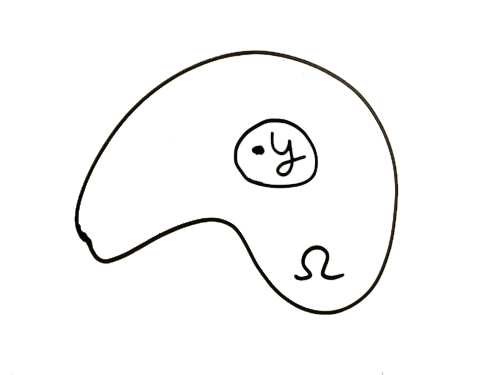
\includegraphics[scale=0.3]{part6.1.png}
\end{center}

В множестве $\Omega \setminus B_\eps (y)$ функция Грина будет гармонической. Для достаточно маленького $\eps$ будет верно

\begin{align*}
	\begin{cases*}
		- \Delta_x G(x,y) = \delta_y, \\
		G(x,y)\Big\rvert_{x \in \partial \Omega} = 0.
	\end{cases*}
\end{align*}
При достаточно маленьком $\eps$ имеем
$$ G(x, y) = \underbrace{\Phi(x-y)}_{\substack{\text{сколь угодно} \\ \text{большая}}} + \underbrace{v^y(x)}_{\substack{\text{гармоническая,} \\ \text{ограниченная}}} \quad \Rightarrow \quad G(x,y)\Big\rvert_{\partial B_\eps (y)} > 0.$$
Функция $G(x,y)$ достигает максимума и минимума на границах, а на границах она неотрицательна. Значит, она неотрицательна всюду.
% как-то хлипко вышло

\end{proof}
\item $ \displaystyle \lim_{x \to y} G(x,y) = + \infty$.
\begin{proof}Видно из доказательства предыдущего свойства.

\end{proof}
\item $G(x, y) = G(y, x)$ - функция Грина симметрична.
\begin{proof}
Пусть
$$ u(x) = G(x,y), \quad v(x) = G(x,z).$$
Рассмотрим два непересекающихся шара $U(y) \subset \Omega$ и $V(z) \subset \Omega$.

\begin{center}
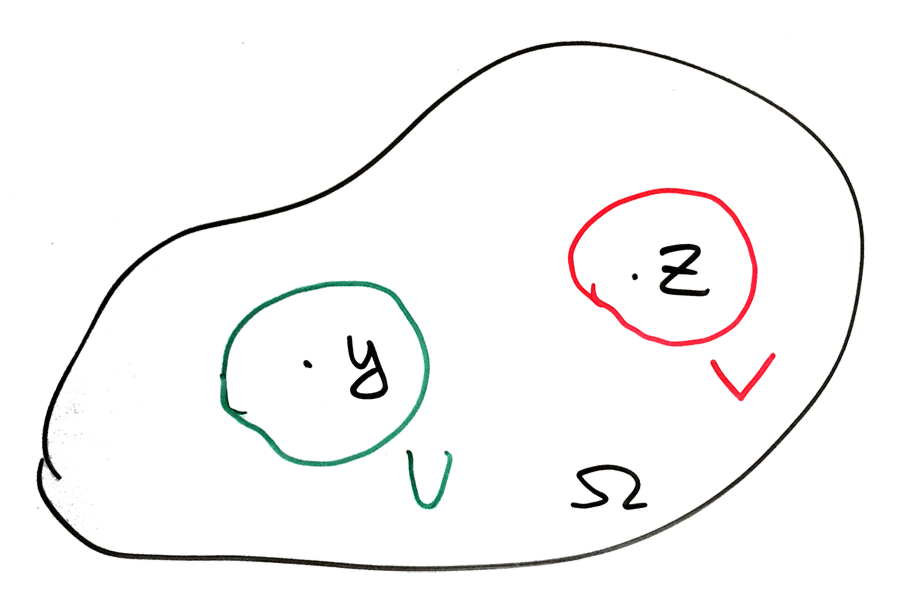
\includegraphics[scale=0.2]{part6.2.png}
\end{center}

Заметим, что верно
\begin{align*}
	- \Delta u = 0\quad \text{в $V$}, \\
	- \Delta v = 0 \quad \text{в $U$}. 
\end{align*}
По второй формуле Грина для $\Omega \setminus (U \cup V)$:
$$ \int \limits_\Omega \underbrace{u \Delta v - v \Delta u}_{=0} \, dx = \int \limits_{\partial U} u \pder[v]{n} - v \pder[u]{n} \, d\sigma + \int \limits_{\partial V} u \pder[v]{n} - v \pder[u]{n} \, d\sigma = 0.$$

Тогда по третьей формуле Грина
\begin{align*}
	v(y) = - \int \limits_{\partial U} u \pder[v]{n} - v \pder[u]{n} \, d\sigma \quad \text{в $U$}, \\
	u(z) = - \int \limits_{\partial V} v \pder[u]{n} - u \pder[v]{n} \, d\sigma \quad \text{в $V$}.
\end{align*}
Подставим последние две формулы в формулу до них:
$$ -v(y) + u(z) = 0 \quad \Rightarrow \quad G(y,z) = G(z,y).$$

\end{proof}

\end{enumerate}

\subsection{Нахождение функции Грина для полупространства}
Для начала рассмотрим $\Omega = \left\{ x_n > 0 \right\} \subset \real^n$ - полупространство.
\begin{note}
Представим, что мы находимся в 18 веке: не будем обращать внимания на формальности, говорящие, что область $\Omega$ должна быть ограниченной.
\end{note}
В нижнем полупространстве находится "земля" (потенциал равен нулю). Поместим заряд в $1$ Кл в точку $y$. Требуется посчитать его потенциал.

Такую задачу можно свести к задаче без заземления: представим, что заземления нет. Далее поставим заряд в $-1$ Кл в точку $y'$, симметричную относительно границы нашего полупространства, и будем рассматривать эту систему.

\begin{center}
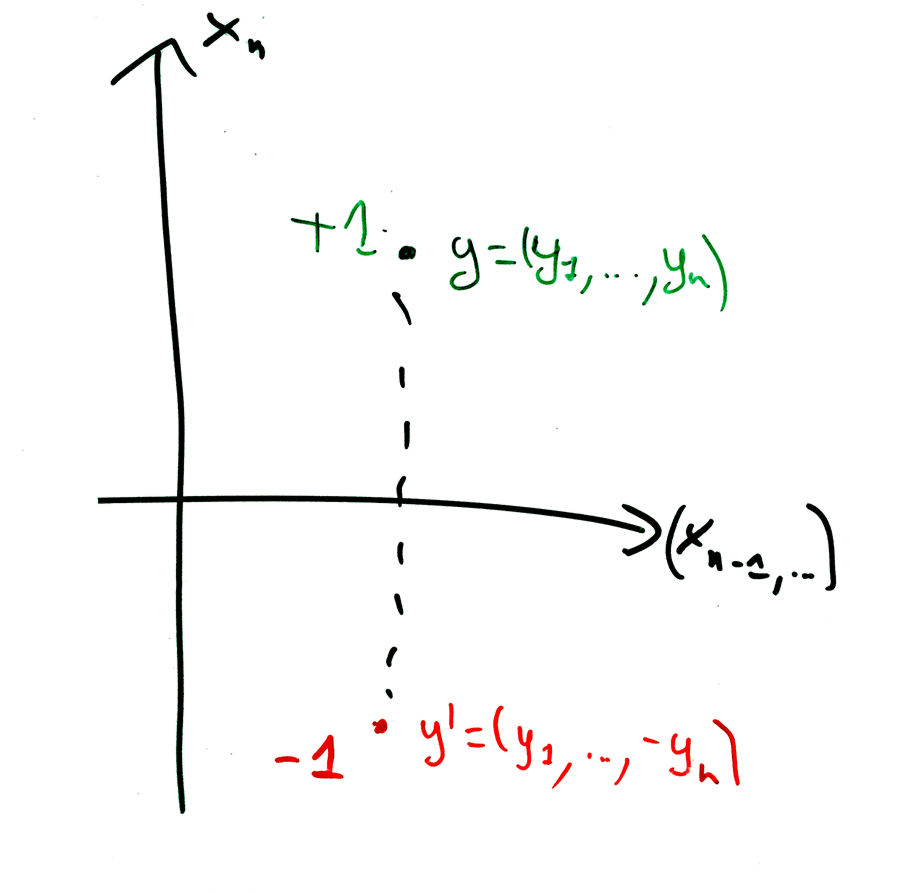
\includegraphics[scale=0.25]{part6.3.png}
\end{center}

Тогда
$$ G(x,y) = \Phi (x-y) - \Phi (x - y'),$$
где
$$ \Phi (x - y) = \frac {1} {n (n-2) \omega_n} \frac {1} {\abs{x-y}^{n-2}}.$$
По геометрическим соображениям потенциал этой системы зарядов на границе полупространства будет равен нулю. В некотором определённом смысле с помощью полученной $G(x,y)$ можно решить задачу Дирихле в полупространстве.

\subsection{Нахождение функции Грина для шара}
Перейдём к шару. Для простоты наш шар это $B_1 (0) \subset \real^n$. Допустим, у нас есть заземлённая граница шара и заряд в $1$ Кл в точке $y$. Создадим систему зарядов, в которой при отсутствии заземлённой границы "фиктивные" заряды компенсируют потенциал имеющегося заряда. Делаем инверсию:
$$ y' = \frac {y} {\abs{y}^2}. $$

Воспользуемся свойством инверсии:
$$ (\abs{y} \cdot \abs{x-y'})^2 = \abs{y}^2 (\abs{x}^2 + \abs{y'}^2 - 2 xy') \stackrel{\abs{x}=1}=(\abs{y}^2 + 1 - 2 x y') = \abs{x-y}^2.$$
То есть,
$$ \abs{y} \cdot \abs{x-y'} = \abs{x-y} \quad \text{при } \abs{x} = 1.$$.

\begin{center}
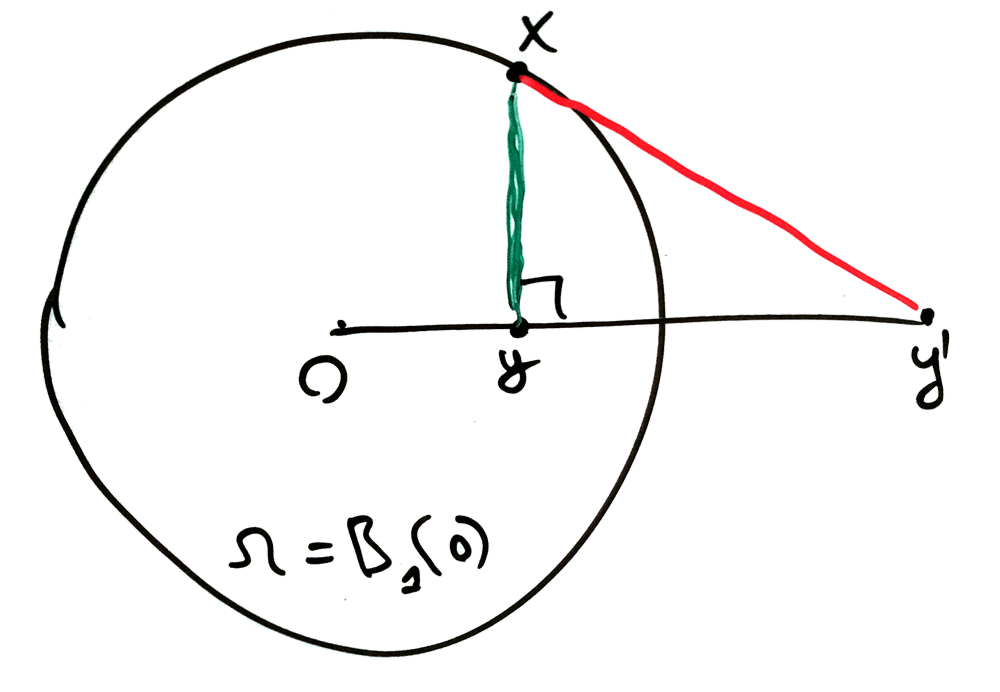
\includegraphics[scale=0.2]{part6.4.png}
\end{center}

Тогда в качестве $G$ возьмём сумму двух кулоновских потенциалов:
$$ G(x,y) = \frac {1} {n (n-2) \omega_n} \left( \frac {1} {\abs{x-y}^{n-2}} - \frac {1} {\abs{y} \cdot \abs{x-y'}^{n-2}} \right).$$
Непосредственно проверяются условия из определения функции Грина:
\begin{align*}
	\begin{cases*}
		- \Delta_x G(x, y) = \delta_y, \\
		G(x, y)\Big\rvert_{\abs{x} = 1} = 0.
	\end{cases*}
\end{align*}
Значит, в результате инверсии мы получили нужный "фиктивный" заряд и нашли функцию Грина для шара. Решим задачу Дирихле для уравнения Лапласа в единичном шаре:

\begin{align*}
	\begin{cases*}
		- \Delta u = 0, \\
		u\Big\rvert_{\partial \Omega} = u_0.
	\end{cases*}
\end{align*}
Считаем:
$$u(y) = - \int \limits_{\partial \Omega} u_0 \pder{n_x} G(x,y) \, d\sigma(x) + \int \limits_\Omega \underbrace{f(x)}_{=0} G(x,y) \, dx = - \int \limits_{\partial B_1 (0)} u_0 k(x, y) \, d\sigma(x),$$
где
$$ k (x,y) = - \pder{n_x} G(x,y) = \frac {1 - \abs{y}^2} {n \omega_n} \frac {1} {\abs{x-y}^n} = - \nabla_x G(x,y) \cdot \underbrace{x}_{\substack{\text{направление} \\ \text{нормали}} } \quad \text{--- ядро Пуассона}.$$

\begin{exercise} Показать, что полученное $u$ - действительно решение.
\end{exercise}
\begin{note}Так как
% TODO: дописать про пронос лапласиана под знак интеграла
$$- \Delta u(y) = \int \limits_{\partial B_1 (0)} u_0 \Delta_y k(x, y) \, d\sigma,$$
то достаточно доказать, что при фиксированном $x$ функция $k$ - гармоническая по второй переменной:
$$ - \Delta_y k(x,y) = 0, \quad \abs{x} = 1.$$
\end{note}

\begin{exercise} Показать, что
$$ \lim_{\substack{y \to x_0 \\ \abs{x_0} = 1}} k(x, y) = 0 \quad x_0 \neq x$$
и
$$ k( x, \cdot) \notin C(\overline{\Omega}) \quad \forall x.$$
\end{exercise}

\begin{note}Пусть $Q$ - матрица поворота. Тогда
$$ u(Qy) = u(y),$$
то есть $u$ радиально симметрична.
\end{note}
\begin{proof}
Посчитаем:
\begin{align*}
	u(Qy) &= \int \limits_{\partial \Omega} \frac {1 - \abs{Qy}^2} {n \omega_n \abs{x-Qy}^n} \, d\sigma(x) = \int \limits_{\partial \Omega} \frac {1 - \abs{y}^2} {n \omega_n \abs{Qx-y}^n} \, d\sigma(x) \stackrel{z = Qx} = \\
	&= \int \limits_{\partial \Omega} \frac {1 - \abs{y}^2} {n \omega_n \abs{z - y}^n} \underbrace {\abs{Q}}_{=1} \, d\sigma(z) = u(y). 
\end{align*}

Мы воспользовались тем, что
\begin{align*}
	\abs{x-Qy}^n = \left( \abs{x-Qy}^2 \right)^{\frac {n} {2}} = (1 + \abs{y}^2 - 2 x Q y)^{\frac {n} {2}} = (1 + \abs{y}^2 - 2Qxy)^{\frac {n} {2}} = \abs{Qx - y}^n
\end{align*}

\end{proof}

\begin{note} $u(y) = 1$.
\end{note}
\begin{proof}
Функция $u$ гармоническая и радиально симметрична. Рассмотрим сферы с центром в нуле и с $y$ на границе:
\begin{center}
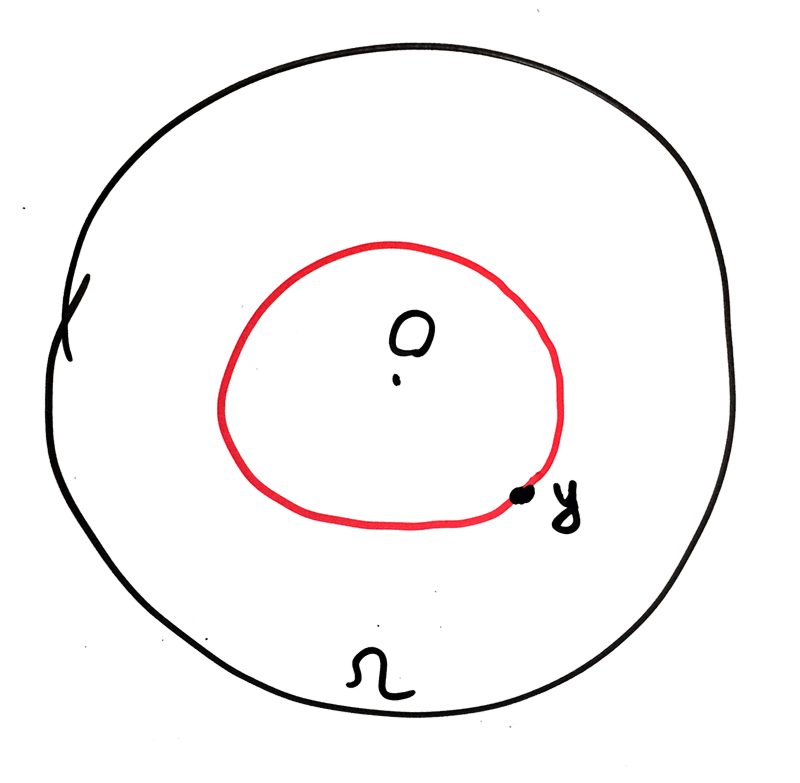
\includegraphics[scale=0.2]{part6.5.png}
\end{center}
На каждой такой сфере функция $u$ константна. По теореме о среднем функция в нуле равна среднему по любой такой сфере. Значит, она константна везде и равна значению в центре:
$$ u(y) = u(0) = \frac {1} {n \omega_n} \int \limits_{\partial B_1 (0)} \frac {1} {\abs{x}^n} \, d\sigma = 1.$$

\end{proof}

\begin{note}
$$\lim_{y \to x_0} u(y) = u_0 (x_0).$$
\end{note}
\begin{proof}
Посчитаем:
\begin{align*}
	|u(y) - u_0(x_0)| &= \left| \, \int \limits_{\partial \Omega} k(x, y) u_0(x) \, d\sigma(x) - u_0(x_0) \int \limits_{\partial \Omega} k(x,y) \, d\sigma(x) \right| = \\
	& = \left| \, \int \limits_{\partial \Omega} k(x,y) (u_0(x) - u_0(x_0)) \, d\sigma(x)\right| \leq \\
	& \leq \int \limits_{\partial \Omega} k(x, y) | u_0(x) - u_0(x_0) | \, d\sigma(x) \leq \\
	& \leq \int \limits_{\partial \Omega \cap B_\eps (x_0)} k(x, y) \delta \, d\sigma(x) + 2 || u_0 ||_\infty \int \limits_{\partial \Omega \setminus B_\eps (x_0)} k(x, y) \, d\sigma(x),
\end{align*}
где 
$$ \eps: \, |x - x_0| \leq \eps \Rightarrow |u_0(x) - u_0(x_0)| \leq \delta $$
и
$$ |u_0 (x) - u_0(x_0)| \leq 2 || u_0 ||_\infty.$$
Знаем, что 
$$ \lim_{y \to x_0} k(x, y) = 0 \quad \text{и} \quad \int \limits_{\partial \Omega \cap B_\eps (x_0)} \leq 1,$$
значит,
$$ \lim_{y \to x_0} |u(y) - u_0(x_0)| \leq \delta \cdot 1 + 0 \quad \forall \eps$$

\end{proof}
% !TEX encoding = UTF-8 Unicode
% лекции 13-14, 19 апреля 2016, начало второй части
\chapter{Соболевские пространства}
% !TEX encoding = UTF-8 Unicode
% лекции 15-16, 2 апреля 2016
% 6. Неравенство Фридрихса.
% 7. Слабая непрерывность линейных операторов. Слабая сходимость в $H_0^1$ и в $L^2$. Слабая непрерывность оператора обобщенного дифференцирования.
% 8. ∗ Существование точки минимума интегрального функционала в $H_0^1$.
% 9. Существование обобщенного решения задачи Дирихле для уравнения Пуассона — вариационный метод. ∗ Метод конечных элементов (метод Рисса).
% 10. Точки минимума выпуклых и строго выпуклых функционалов. Единственность экстремали. Единственность обобщенного решения задачи Дирихле для уравнения Пуассона - вариационный метод.
% 11. Существование и единственность обобщенного решения задачи Дирихле для уравнения Пуассона — использование теоремы Рисса. ∗∗ Регулярность обобщенного решения (существование классического решения) — формулировка.
% 12. Непрерывная обратимость оператора $-\Delta : H_0^1 \to L^2$.

% 6. Неравенство Фридрихса.
\subsection{Неравенство Фридрихса}
\begin{theorem} Пусть $\Omega \subset \real^n$ - ограниченная область, $u \in \m{H01Om}$. Тогда
$$ \int \limits_\Omega u^2 \, dx \leq C_\Omega \int \limits_\Omega |\nabla u|^2 \, dx.$$
\end{theorem}
\begin{proof} Пространство $C_0^\infty(\Omega)$ плотно в $\m{H01Om}$, так что достаточно доказать для него, а потом перейти к пределу.

Пусть $u \in C_0^\infty(\Omega)$. Существует такое $a$, что $\Omega \subset (-a,a)^n.$ Зафиксируем все координаты, кроме $i$-ой. Тогда по неравенству Гёльдера
\begin{align*}
|u(x)| &\leq \int \limits_{-a}^x \Bigl\lvert \pder{x_i} u(x_1, ..., \xi_i, ..., x_n) \Bigr\rvert \, d \xi_i \\ \\
& \leq \left( \int \limits_{-a}^a \Bigl\lvert \pder{x_i} u(x_1, ..., \xi_i, ..., x_n)  \Bigr\rvert^2 \, d\xi_i\right)^{1/2} \sqrt{2a},\\
|u(x)|^2 &\leq 2a \int \limits_{-a}^a | u_{x_i} (x_1, ..., \xi_i, ..., x_n) | \, d\xi_i.
\end{align*}
Интегрируем по всем остальным координатам по $(-a, a)$. После интегрирования по всем координатам, кроме $i$-ой, получим норму $u_{x_i}$ в квадрате. Проинтегрировав её по $x_i$, получим дополнительный множитель $2a$:
$$ \norm*{2}{u}^2 \leq 4a^2 \norm*{2}{u_{x_i}} \leq 4a^2 \norm*{2}{\nabla u}^2.$$
Таким образом,
$$\norm*{2}{u} \leq C_\Omega \norm*{2}{\nabla u},$$
где константа зависит только от диаметра области.

Пусть теперь $u \in \m{H01Om}$. Аппроксимируем:
$$ \exists \{u_k \} \subset C_0^\infty(\Omega) : u_k  \conv{H1}{} u,$$
то есть,
$$ \norm{H1}{u_k - u}^2 = \norm*{2}{u_k - u}^2 + \norm*{2}{\nabla u_k - \nabla u}^2 \conv{}{} 0,$$
откуда
$$\norm*{2}{u_k} \conv{}{} \norm*{2}{u}, \quad \norm*{2}{\nabla u_k} \conv{}{} \norm*{2}{\nabla u}.$$
Итого,
$$ \norm*{2}{u} \leq C \norm*{2}{\nabla u},$$
что и требовалось доказать.
\end{proof}

\begin{note}
Впервые нам реально понадобилась ограниченность области $\Omega$.
\end{note}

\begin{note}
На самом деле мы пользуемся ограниченностью только по одному направлению. 
\end{note}

% 7. Слабая непрерывность линейных операторов. Слабая сходимость в $H_0^1$ и в $L^2$. Слабая непрерывность оператора обобщенного дифференцирования.
\subsection{Слабая сходимость в гильбертовом пространстве}
Вспомним некоторые сведения из функционального анализа.
\begin{definition}
Пусть $H$ - гильбертово пространство. Последовательность $\{x_k \} \subset H$ называется слабо сходящейся к $x$, если
$$\scalprod*{H}{x_k}{y} \conv*{H}{} \scalprod*{H}{x}{y} \quad \forall y \in H,$$
и обозначается
$$ x_k \wkconv*{H}{} x.$$
\end{definition}

\begin{note}
Слабая сходимость слабее сильной:
$$ x_k \conv{}{} x \quad \Rightarrow \quad x_k \wkconv{}{} x.$$
\end{note}

\begin{note}
Обратное неверно.
\end{note}

\begin{example} Пусть $H = L^2(0, \pi)$, функция $f \in H$. Тогда $f$ представима в виде сходящегося в смысле $H$ ряда
$$ f = \sum_{k=1}^\infty a_k \sin kx.$$
Обозначим $u_k = \sin kx$. Известно равенство Парсеваля:
$$ \sum_{k=1}^\infty a_k^2 = \frac {2} {\pi} \norm*{2}{f}^2.$$
Значит, $|a_k| \to 0$, где
$$ a_k = \frac {\scalprod*{H}{f}{u_k}} {\norm*{H}{u_k}^2} = \frac {2} {\pi} \scalprod*{H}{f}{u_k} \to 0.$$
Это выполняется для всех $f$. По определению слабой сходимости
$$ u_k \wkconv*{H}{} 0 \quad \Leftrightarrow \quad \sin kx \wkconv*{H}{k \to \infty} 0.$$
Но сильно $\{ u_k \}$ никуда не сходится хотя бы потому, что $\displaystyle \norm*{H}{u_k} = \frac {\pi} {2}$.
\end{example}

\begin{note}
Слабая топология в гильбертовом пространстве не задаётся никакой метрикой. Однако, шар в сепарабельном гильбертовом пространстве со слабой топологией метризуем.
\end{note}

% TODO: доказать
\begin{note}[Слабая компактность шара] Пусть $H$ - сепарабельное гильбертово пространство. Тогда
$$ \{ x_k \} \subset H : |x_k| \leq C \quad \Rightarrow \quad \exists \{ x_{k_n} \} : x_{k_n} \wkconv{}{} x.$$
\end{note}

% TODO: доказать
\begin{note} В сепарабельном гильбертовом пространстве норма слабо полунепрерывна снизу:
$$x_k \wkconv*{}{} x \quad \Rightarrow \quad \norm{}{x_k} \leq \lim \inf \norm*{}{x_k}.$$
\end{note}

% TODO: замкнутое выпуклое подмножество гильбертова пр-ва слабо замкнуто

\begin{note} Непрерывный линейный оператор $A$ между гильбертовыми пространствами $H_1$ и $H_2$  сохраняет слабую сходимость:
$$ x_k \wkconv*{H_1}{} x \quad \Rightarrow \quad Ax_k \wkconv*{H_2}{} Ax.$$
\end{note}
\begin{proof}
$$ \scalprod*{H_2}{A x_k} {y} = \scalprod*{H_1}{x_k}{A^*y} \conv*{H_1}{} \scalprod*{H_1}{x}{A^*y} = \scalprod*{H_2}{Ax}{y}.$$

\end{proof}

\subsection{Слабая сходимость в $\m{L2}$ и в $\m{H01}$}
Пусть $\Omega \subset \real^n$ - область. Рассмотрим оператор вложения
$$\dot{\iota} : \m{H01Om} \longrightarrow \m{L2Om},$$
$$\dot{\iota}(u) := u.$$

Оператор $\dot{\iota}$ непрерывен, так как
$$ \norm*{2}{\dot{\iota}}(u)^2 = \norm*{2}{u}^2 \leq \norm{H1}{u}^2.$$
Следовательно,
$$ u_k \wkconv{H1}{} u \quad \Rightarrow \quad u_k \wkconv{L2}{} u.$$

Рассмотрим оператор обобщённого дифференцирования по $i$-ой переменной:
$$ \pder{x_i} : \m{H01Om} \longrightarrow \m{L2Om}.$$
Нам уже известно, что он линеен и непрерывен. Значит, он тоже сохраняет слабую сходимость:
$$ u_k \wkconv{H1Om}{} u \quad \Rightarrow \quad \pder[u_k]{x_i} \wkconv{L2Om}{} \pder[u]{x_i}.$$

% 8. ∗ Существование точки минимума интегрального функционала в $H_0^1$.
\subsection{Существование точки минимума интегрального функционала в $\m{H01}$}
\begin{lemma} В $\m{H1Om}$ функционал $F$ слабо полунепрерывен снизу:
$$u_k \wkconv{H1}{} u \quad \Rightarrow \quad F(u) \leq \lim \inf F(u_k).$$
\end{lemma}
\begin{proof} Прежде всего заметим, что
$$ \int \limits_\Omega f u_k \, dx = \scalprod*{2}{f}{u_k} \wkconv{L2}{} \scalprod*{2}{f}{u} =\int \limits_\Omega f u \, dx.$$
Посмотрим на обобщённый градиент:
\begin{align*}
0 \leq | \nabla (u_k - u) |^2 &= | \nabla u_k - \nabla u |^2 = |\nabla u_k|^2 + |\nabla u|^2 - 2 \nabla u_k \cdot \nabla u \\
&= |\nabla u_k|^2 - |\nabla u|^2 + 2 \nabla u \cdot (\nabla u - \nabla u_k),
\end{align*}
$$ |\nabla u_k|^2 - |\nabla u|^2 \geq 2 \nabla u \cdot (\nabla u_k - \nabla u).$$
Проинтегрируем:
$$ \int \limits_\Omega \frac {| \nabla u_k|^2} {2} \, dx - \int \limits_\Omega \frac {| \nabla u|^2} {2} \, dx \geq \int \limits_\Omega \nabla u \cdot (\nabla u_k - \nabla u) \, dx = \sum_{j=1}^n \int \limits_\Omega u_{x_j} \left( \pder[u_k]{x_j} - u_{x_j} \right) .$$
Заметим, что
$$ \pder[u_k]{x_j} - \pder[u]{x_j} \wkconv{L2}{} 0 \quad \Rightarrow \quad u_{x_j} (\hdots) \conv{}{k \to \infty} 0,$$
то есть,
$$ \lim \inf \frac {1} {2} \int \limits_\Omega |\nabla u_k|^2 \, dx \geq \frac {1} {2} \int \limits_\Omega |\nabla u|^2 \, dx.$$
Итого
\begin{align*}
\lim \inf F(u_k) &= \lim \inf \left( \frac {1}{2} \int \limits_\Omega |\nabla u_k|^2 \, dx - \int \limits_\Omega fu_k \, dx \right) \\
&\geq \lim \inf \frac {1} {2} \int \limits_\Omega |\nabla u_k|^2 \, dx - \lim \inf \int \limits_\Omega fu_k \, dx \\
&\geq \frac {1} {2} \int \limits_\Omega |\nabla u|^2 \, dx - \int \limits_\Omega fu \, dx = F(u),
\end{align*}
что и требовалось доказать.

\end{proof}

\begin{theorem}[Существование точки минимума интегрального функционала] Пусть $\Omega \subset \real^n$ - ограниченная область, $f \in L^2(\Omega)$, и задан фунцкионал 
$$F(u) = \frac {1} {2} \int \limits_\Omega | \nabla u |^2 \, dx - \int \limits_\Omega fu \, dx.$$
Тогда существует $u \in \m{H01Om}$ такая, что 
$$ F(u) = \inf_{v \in \m{H01Om}} F(v).$$
\end{theorem}
\begin{note} Функционал $F$ определён на $\m{H01Om}$: если понимать градиент как обобщённый, то выражение имеет смысл.
\end{note}
\begin{proof}[Доказательство теоремы]
Воспользуемся методом Тонелли. Рассмотрим минимизирующую последовательность $\{ u_k \} \subset \m{H01Om}$:
$$ F(u_k) \conv{}{} \inf_{\m{H01Om}} F.$$
Заметим, что верно (например, $C = 0$ при $u \equiv 0$):
$$F(u_k) = \frac {1} {2} \int \limits_\Omega | \nabla u_k |^2 \, dx - \int \limits_\Omega f u_k \, dx \leq C.$$
Заметим, что :
\begin{align*}
F(u_k) &\stackrel{\text{(а)}}{\geq} \frac {1} {2} \norm*{2}{\nabla u_k}^2 - \frac{1} {2 \eps} \norm*{2}{f}^2 - \frac{\eps^2}{2} \norm*{2}{u_k}^2 \\
& \stackrel{\text{(б)}}{\geq} \frac {1} {2} \norm*{2}{ \nabla u_k } - \frac {1} {2\eps} \norm*{2}{ u_k}^2 - \frac {\eps^2} {2} C_\Omega \norm*{2}{ \nabla u_k}^2.
\end{align*}
В первом переходе воспользовались тем, что 
$$ ab \leq \frac {a^2 + b^2} {2} \quad \Rightarrow \quad \Biggl\lvert \int \limits_\Omega \frac {f} {\eps} \eps u_k \, dx \Biggr\rvert \leq \frac {1} {2} \left( \frac {1} {\eps^2} \norm*{2}{f}^2 + \eps^2 \norm*{2}{u_k}^2 \right).$$
Имеем:
$$C \geq F(u_k) \geq \frac {1} {2} \left(1 - \eps^2 C_\Omega \right) \norm*{2}{ \nabla u_k }^2 - \frac {1} {2 \eps^2} \norm*{2}{f}^2.$$
Тогда
$$ \frac {1} {2} \left( 1 - \eps^2 C_\Omega \right) \norm*{2}{ \nabla u_k}^2 \leq \underbrace {C + \frac {1} {2 \eps^2} \norm*{2}{f}^2}_{=C}.$$
Можно выбрать такое $\eps$, что $ \eps^2 C_\Omega < 1$. Тогда 
$$ \norm*{2}{\nabla u_k}^2 \leq C,$$
и
$$ \norm*{2}{u_k}^2 \leq C_\Omega \norm*{2}{ \nabla u_k}^2 \leq C.$$
Таким образом, $\{ u_k \}$ ограничена в $\m{H01Om}$:
$$ \norm{H1}{u_k} \leq C,$$ 
то есть, $\{ u_k \}$ лежит в некотором шаре в $\m{H1Om}$.

В стандартной топологии шар не компактен, зато компактен в слабой топологии. Значит, существует такая подпоследовательность $\left\{ u_{k_m} \right\} \subset \left\{ u_k \right\}$, что 
$$u_{k_m} \wkconv{H1Om}{m \to \infty} u \in \m{H01Om}.$$ 
Заметим, что слабая сходимость в $\m{H1Om}$ влечёт слабую сходимость в $\m{L2Om}$, а оператор обобщённого дифференцирования слабо непрерывен. Значит,
$$ u_{k_m} \wkconv{L2Om}{} u, \quad \pder[u_{k_m}]{x_i} \wkconv{L2Om}{} \pder[u]{x_i},$$
и
$$ \int \limits_\Omega f u_{k_m} \, dx \longrightarrow \int \limits_\Omega fu \, dx.$$

Первое слагаемое функционала непрерывно, а второе слагаемое по лемме полунепрерывно снизу. Значит,
$$ F(u) \leq \lim \inf \left( \int \limits_\Omega | \nabla u_{k_m}|^2 \, dx - \int \limits_\Omega f u_{k_m} \, dx \right) = \inf F.$$

Итого,
$$ F(u) = \inf F.$$

\end{proof}

Резюмируя: мы рассмотрели прозвольную минимизирующую последовательность для функционала. Потом достаточно примитивным трюком доказали, что она ограниченная по норме в $H^1$, используя неравенство Фридрихса. Значит, она содержит слабо сходящуюся подпоследовательность, она тоже минимизирующая. Функционал слабо (полу)непрерывен снизу, значит, в пределе получаем нижний предел $u_k$, а это в точности инфимум.

% 9. Существование обобщенного решения задачи Дирихле для уравнения Пуассона — вариационный метод. ∗ Метод конечных элементов (метод Рисса).
\subsection{Существование обобщённого решения - вариационный метод}
\begin{theorem} Пусть $u \in \m{H01Om}$ - минимум $F$, тогда $u$ - решение уравнения Пуассона:
$$- \Delta u = f.$$
\end{theorem}
\begin{proof} Если $u$ - минимум $F$, то
$$F'(u)v = \int \limits_\Omega \nabla u \cdot \nabla v \, dx - \int \limits_\Omega f v \, dx = 0 \quad \forall v \in \m{H01Om}.$$
В частности, это выполняется и для всех $v$ из $C_0^\infty (\Omega)$. Тогда
\begin{align*}
	0 &= \int \limits_\Omega \nabla u \cdot \nabla v \, dx - \int \limits_\Omega f v \, dx = \sum_{k=1}^n \int \limits_\Omega u_{x_k} v_{x_k} \, dx - \int \limits_\Omega f v \, dx \\
	&= \sum_{k=1}^n \action{v_{x_k}, u_{x_k}} - \action{v,f} = - \sum_{k=1}^n \action{v, u_{x_k x_k}} - \action{v,f} \\
	&= - \action{v, \underbrace{\Delta u}_{\text{обобщ}}} - \action{v, f} = \action{v, -\Delta u -f} = 0.
\end{align*}
Значит, минимум функционала $F$ удовлетворяет уравнению Пуассона в обобщённом смысле 
$$ - \Delta u = f.$$

\end{proof}

А минимум существует по предыдущей теореме. Значит, решение уравнения Пуассона  существует.

В дальнейшем нам пригодится следующая лемма.
\begin{lemma}
Если $-\Delta u = f$ в обобщённом смысле, и $u \in \m{H01Om}$, то
$$ \int \limits_\Omega \nabla u \cdot \nabla v \, dx - \int \limits_\Omega fv \, dx = 0 \quad \forall v \in \m{H01Om}.$$
\end{lemma}
\begin{proof} Надо доказать в обратную сторону предыдущую цепочку равенств. Из условия леммы следует, что 
$$ \action{\varphi, -\Delta u} = \action{\varphi, f} \quad \forall \varphi \in C_0^\infty(\Omega).$$
Тогда 
\begin{align*}
- \sum_{k=1}^n \action{\varphi, u_{x_k x_k}} &= \sum_{k=1}^n \action{\varphi_{x_k}, u_{x_k}} = \sum_{k=1}^n \int \limits_\Omega \varphi_{x_k} u_{x_k} \, dx \\
&= \int \limits_\Omega \nabla \varphi \cdot \nabla u \, dx = \int \limits_\Omega \varphi f \, dx \quad \forall \varphi \in C_0^\infty(\Omega).
\end{align*}
Теперь рассмотрим $v$ из $\m{H01Om}$. По определению,
$$ \exists \{ \varphi_k \} \subset C_0^\infty(\Omega) : \varphi_k \conv{H1}{} v.$$
Значит, по непрерывности оператора вложения
$$ \varphi_k \conv{L2}{} v, \quad \pder[\varphi_k]{x_j} \conv{L2}{} \pder[v]{x_j}, \quad \nabla \varphi_k \conv{L2}{} \nabla v.$$

В пределе получаем
$$ \int \limits_\Omega \nabla v \cdot \nabla u \, dx - \int \limits_\Omega fv \, dx = 0.$$

\end{proof}

\begin{note} Мы доказали равносильность задач! Если $f$ из $\m{L2Om}$, $u$ из $\m{H01Om}$, то
$$ -\Delta u = f \quad \Leftrightarrow \quad \int \limits_\Omega \nabla v \cdot \nabla u \, dx = \int \limits_\Omega fv \, dx \quad \forall v \in \m{H01Om}.$$
\end{note}

Таким образом, подобное $F$ интегральное условие является обобщённым аналогом условия Дирихле.


\subsection{Метод конечных элементов} Пусть $\Omega \subset \real^2$ - ограниченная область. Задача Дирихле для уравнения Пуассона в обобщённом смысле эквивалентентна вариационной задаче
$$ F(u) = \frac {1}{2} \int \limits_\Omega |\nabla u|^2\ \,dx - \int \limits_\Omega fu \, dx \rightarrow \min.$$
Знаем, что у $F$ существует минимум. Тогда у задачи Дирихле для уравнения Пуассона существует решение (чуть далее мы докажем, что минимум и решение единственны. Вариационный метод подсказывает, как можно найти приближённое решение.

Триангулируем $\Omega$ - разобьём её на $m$ достаточно малых треугольников. Скажем, что на $k$-ом треугольнике действует линейная функция $u_k$, приближающая $u$ в этой части области. Линейная функция на треугольнике определяется своими значениями в вершинах треугольника. Таким образом, неизвестная функция $u_k$ заменяется на неизвестные функции $u_k$, которые определяются неизвестными значениями в узлах треугольников. В узлах на границе положим $u = 0$. Тогда $F$ - квадратичная функция на $\real^m$, она выпукла.

Таким образом, задача свелась к нахождению минимума квадратичной функции на конечномерном пространстве. Если приравнять её градиент к нулю, то полученное соотношение можно представить в виде системы линейных уравнений порядка $m$ с трёхдиагональной матрицей.

Можно доказать, что при дальнейшем дроблении области на треугольники полученное приближение будет сходиться к $u$ по энергетической норме.  

В $\real^n$ вместо треугольников пространство следует разбивать на симплексы.

% 10. Точки минимума выпуклых и строго выпуклых функционалов. Единственность экстремали. Единственность обобщенного решения задачи Дирихле для уравнения Пуассона - вариационный метод.
\subsection{Единственность обобщённого решения - вариационный метод}

\begin{definition} Вещественный функционал $G$ на гильбертовом пространстве, удовлетворяющий условию
$$ G(\lambda_1 u_1 + \lambda_2 u_2) \leq \lambda_1 G(u_1) + \lambda_2 G(u_2), \quad \lambda_1,\lambda_2 \geq 0, \quad \lambda_1 + \lambda_2 = 1,$$
называется выпуклым.
\end{definition}

\begin{exercise}
$$ F(u) = \frac {1} {2} \int \limits_\Omega |\nabla u|^2 \, dx - \int \limits_\Omega fu \, dx \quad \text{--- выпуклый.}$$
\end{exercise}

\begin{definition} Вещественный функционал $G$ на гильбертовом пространстве, удовлетворяющий условию
$$ G(\lambda_1 u_1 + \lambda_2 u_2) < \lambda_1 G(u_1) + \lambda_2 G(u_2), \quad \lambda_1,\lambda_2 > 0, \quad \lambda_1 + \lambda_2 = 1,$$
называется строго выпуклым.
\end{definition}

\begin{exercise}
Если $G$ --- строго выпуклый, то у него единственная точка минимума.
\end{exercise}

Докажем единственность. Нам понадобится следующая абстрактная лемма:

\begin{lemma} Пусть $F$ - выпуклый вещественный функционал на гильбертовом пространстве $H$, у которого всюду существует первая вариация
$$ \exists F'(u) v \quad \forall v \in H,$$ и пусть имеется $u$ из $\m{H01Om}$ такое, что
$$ F'(u)v = 0 \quad \forall v \in H.$$
Тогда $u$ - точка минимума $F$:
$$ F(u) = \inf_{\m{H01Om}} F. $$
% ???? не странно ли записано условие?
\end{lemma}
\begin{proof}
Рассмотрим выпуклую функцию
$$ g(t) = F(u+tv) \quad t\in \real.$$
Тогда
$$F'(u)v = \frac{d}{dt} F(u+tv)\Big\rvert_{t=0} = g'(0),$$
и $g(t)$ лежит выше касательной:
$$g(t) \geq g(0) + tg'(0) \quad \forall t \in \real.$$
Рассмотрим такое $w \in H$, что
$$ w = u + tv \quad \Rightarrow \quad v = \frac {w-u} {t}.$$
Тогда
$$ F(w) \geq F(u) + t F'(u) \frac{w-u}{t} = F(u) + F'(u)(w-u).$$
Итого
$$ F'(u)(w-u) = 0 \quad \Rightarrow F(u) \leq F(w) \quad \forall w,$$
значит, $u$ - минимум $F$.

\end{proof}
Теперь мы готовы доказать
\begin{theorem}
Если $u \in \m{H01Om}$ удовлетворяет уравнению
$$ - \Delta u = f,$$
то $$F(u) = \min_{\m{H01Om}} F.$$ 
\end{theorem}
\begin{proof}
Задача Дирихле для уравнения Пуассона эквивалентна задаче
$$F(u) = \int \limits_\Omega \nabla u \cdot \nabla v \, dx - \int \limits_\Omega fu \, dx = 0.$$
У $F$ по любому направлению существует производная Гато $F'(u)v$. Рассмотрим $u$ такое, что 
$$ F'(u) v = 0 \quad \forall v.$$
Тогда по второй лемме $u$ - минимум $F$.

\end{proof}

Таким образом, мы доказали, что уравнение Пуассона имеет единственное решение, совпадающее с минимумом функционала $F$.

% 11. Существование и единственность обобщенного решения задачи Дирихле для уравнения Пуассона — использование теоремы Рисса. ∗∗ Регулярность обобщенного решения (существование классического решения) — формулировка.

\subsection{Существование и единственность обобщённого решения - использование теоремы Рисса}

Пусть $\Omega \subset \real^n$ - ограниченная область, $f$ из $\m{L2Om}$, и поставлена задача Дирихле для уравнения Пуассона:
\begin{align*}
\begin{cases*}
	- \Delta u = f, \\
	u \in \m{H01Om}.
\end{cases*}
\end{align*}
При помощи вариационного метода мы доказали существование и единственность решения. Докажем то же самое, опираясь на теорему Рисса.

\begin{reminder}[Теорема Рисса] Пусть $H$ - гильбертово пространство, $f$ - непрерывный линейный функционал на $H$. Тогда существует единственный $y \in H$ такой, что 
$$ f(x) = \scalprod*{H}{y}{x} \quad \forall x \in H.$$
То есть, любой линейный функционал на $H$ есть скалярное произведение с некоторым $y$ из $H$.
Кроме того,
$$ \norm*{H}{y} = \norm*{H^*}{f}.$$
\end{reminder}

\begin{lemma}[Лакс-Мильграм] Пусть $\widehat{H}$ и $H$ --- гильбертовы пространства и первое непрерывно вложено во второе:
$$ \widehat{H} \hookrightarrow H. $$
Тогда
$$ \forall y \in H \quad \exists ! x \in \widehat{H}: \scalprod*{\widehat{H}}{x}{z} = \scalprod*{H}{y}{z} \quad \forall z \in \widehat{H}.$$
\end{lemma}
\begin{proof}
Пусть $y \in H$. Рассмотрим функционал
\begin{gather*}
f_y : \widehat{H} \longrightarrow \real, \\
f_y(z) := \scalprod*{H}{y}{z}.
\end{gather*}
Очевидно, он линеен. Проверим непрерывность:
$$ |f_y(z)| = | \scalprod*{H}{y}{z} \leq \norm*{H}{y} \cdot \norm*{H}{z} \leq \norm*{H}{y} \cdot \norm*{\widehat{H}}{z} C = C_y \norm*{\widehat{H}}{z}.$$
Функционал $f_y$ непрерывен на $\widehat{H}$. Тогда по теореме Рисса в $\widehat{H}$
$$ \exists ! \, x \in \widehat{H}: \scalprod*{\widehat{H}}{x}{z} = f_y(z) = \scalprod*{H}{y}{z} \quad \forall z \in \widehat{H}.$$

\end{proof}

\begin{note}
Фактически, мы определили оператор $A$:
\begin{gather*}
A : H \longrightarrow \widehat{H}, \\
Ay = x, \quad \scalprod*{H}{y}{z} = \scalprod*{\widehat{H}}{x}{z}.
\end{gather*}
Очевидно, он линеен. Покажем, что он непрерывен. Для начала,
$$ | \scalprod*{\widehat{H}}{x}{z} | = | \scalprod*{H}{y}{Z} | \leq C \norm*{H}{y} \cdot \norm*{\widehat{H}}{z}.$$
Отсюда
$$ \frac {| \scalprod*{\widehat{H}}{x}{z} |} {\norm*{\widehat{H}}{z}} \leq C \norm*{H}{y} \quad \Rightarrow \quad \sup_{z \in \widehat{H}} \frac {| \scalprod*{\widehat{H}}{x}{z} |} {\norm*{\widehat{H}}{z}} \leq C \norm*{H}{y} \quad \Rightarrow \quad \norm*{\widehat{H}}{x} \leq C \norm*{H}{y}.$$
То есть,
$$ \norm*{\widehat{H}}{Ay} \leq C \norm*{H}{y} \quad \Rightarrow \quad A \text{ --- непрерывный}.$$
\end{note}


\begin{theorem} Пусть $f$ из $\m{L2Om}$. Тогда обобщённое решение задачи Дирихле для уравнения Пуассона существует и единственно.
\end{theorem}
\begin{proof} Здесь
$$ H = \m{L2Om}, \quad \widehat{H} = \m{H01Om}.$$
Введём новую норму в $\widehat{H}$:
$$\norm*{\widehat{H}}{u} = \sqrt{\int \limits_\Omega | \nabla u |^2 \, dx } = \norm*{2}{\nabla u}.$$
Эта норма называется энергетической. Очевидно,
$$ \norm*{2}{\nabla u} = \norm*{\widehat{H}}{u} \leq \norm{H1}{u}.$$
В то же время,
$$ \norm*{2}{u} \leq C \norm*{2}{\nabla u} \quad \Rightarrow \quad \norm*{H1}{u} \leq C \norm*{2}{\nabla u} = C \norm*{\widehat{H}}{u}.$$
Значит, энергетическая норма эквивалентна стандартной, и $\widehat{H}$ --- сепарабельное гильбертово пространство. В то же время, вложение $\widehat{H} \hookrightarrow H$ непрерывно:
$$ \norm*{H}{u} = \norm*{2}{u} \leq C \norm*{2}{\nabla u} = C \norm*{\widehat{H}}{u}.$$
Применяем лемму. Для любого $f$ из $\m{L2Om}$ 
$$ \exists! \, u \in \m{H01Om}: \scalprod{H01}{u}{v} = \scalprod{L2}{f}{v} \quad \forall v \in \m{H01Om}.$$
В интегральной форме: существует такой $f$ из $\m{L2Om}$, что
$$ \exists ! u \in \m{H01Om} : \int \limits_\Omega \nabla u \cdot \nabla v \, dx = \int \limits_\Omega f v \, dx \quad \forall v \in \m{H01Om},$$
а это равносильно существованию и единственности решения задачи Дирихле для уравнения Пуассона.

\end{proof}

Недостаток этого подхода заключается в том, что он неконструктивен.
% ????????????
% ∗∗ Регулярность обобщенного решения (существование классического решения) — формулировка.

\subsection{Непрерывная обратимость лапласиана}
% 12. Непрерывная обратимость оператора $-\Delta : H_0^1 \to L^2$.

\begin{theorem}
Пусть $\Omega \subset \real^n$ - ограниченная область. Для любого $f$ из $\m{L2Om}$ существует единственное $u$ из $\m{H01Om}$ такое, что
$$ - \Delta u = f \quad \Rightarrow \quad u = (-\Delta)^{-1} f.$$
Значит, определён оператор
$$ (-\Delta)^{-1}: \m{L2Om} \longrightarrow \m{H01Om}.$$
Этот оператор непрерывен.
\end{theorem}
\begin{proof}
Очевидно, этот оператор линеен. Нам нужно доказать, что
$$ \norm{H1}{(-\Delta)^{-1} f} \leq C \norm*{2}{f}, \quad \text{или, что то же самое,} \quad \norm{H1}{u} \leq C\norm*{2}{f}.$$
Если $u$ - решение уравнения Пуассона, то 
$$ \int \limits_\Omega \nabla u \cdot \nabla v \, dx = \int \limits_\Omega fv \, dx \quad \forall v \in \m{H01Om}.$$
В частности, при $v= u$
\begin{align*}
\norm*{2}{\nabla u}^2 = \int \limits_\Omega |\nabla u|^2 \, dx = \int \limits_\Omega fu \, dx \leq \norm*{2}{f} \cdot \norm*{2}{u} \leq C \norm*{2}{f} \cdot \norm*{2}{\nabla u}
\end{align*}
Сначала мы воспользовались неравенством Гёльдера, а потом неравенством Фридрихса. Тогда
$$ \norm*{2}{\nabla u} \leq C \norm*{2}{f} \quad \text{и} \quad \norm*{2}{u} \leq C\norm*{2}{f}.$$
Итого,
$$ \norm{H1}{u} = \sqrt{\norm*{2}{u}^2 + \norm*{2}{\nabla u}^2} \leq C \norm*{2}{f},$$
что и требовалось доказать.

\end{proof}
% !TEX encoding = UTF-8 Unicode
% лекции 17-18, 9 апреля 2016
% 13. Непрерывность и компактность интегрального оператора в $L^2$ с непрерывным ядром.
% 14. Непрерывность интегрального оператора в $L^2$ со слабой особенностью.
% 15. Замкнутость класса компактных линейных непрерывных операторов. Компактность интегрального оператора в $L^2$ со слабой особенностью.
% 16. Компактность вложения $H_0^1 \subset L^2$ (теорема Реллиха).
% 17. Теорема Фредгольма для компактных самосопряженных операторов в гильбертовом пространстве.
% 18. Сведение задачи Дирихле для уравнения $−\Delta u + \lambda u = f$ к уравнению Фредгольма второго рода с самосопряженным, компактным, положительным оператором. Теорема об альтернативе.

% отступление про интегральные операторы, инт оператор T
% вспомнить теорему асколи-арцела
% теорема: K \in C( \overline{\Omega} \times \overline{\Omega}), T \in L(L^2, L^2) и T компактен
% следствие про операторы со слабой особенностью: оператор с ядром со слабой особенностью является линейным ограниченным оператором

% теорема: A = \int k u, где k - ядро со слабой особенностью, компактен
% факт из ф.а.: предкомпакт <=> сущ. кон. \eps-сеть (с док-вом)

% лемма про гладкую функцию с компактным носителем
% обобщение на функцию из H_0^1

% доказательство теоремы реллиха-кондрашова (мы доказали что-то с её помощью, а потом вводили необходимый мат.аппарат для доказательства собственно теоремы)

% свойства оператора K = i o (-\Delta)^{-1}

% теорема Фредгольма о компактном операторе (альтернатива фредгольма)

% спектр интегрального оператора
% !TEX encoding = UTF-8 Unicode
% лекция 19, 16 апреля 2016, конец курса
% 19. Множество собственных чисел самосопряженных компактных положительных операторов.
% 20. Собственные векторы самосопряженных компактных положительных операторов и полные ортогональные системы векторов.
% 21. Собственные функции лапласиана и полные ортогональные системы векторов в $L^2$ и в $H_0^1$.
% 22. Собственные числа и собственные функции лапласиана. Первое собственное число.
% 23. Разрешимость уравнения $− \Delta u + \lambda u = f$.
% 24. Свойства первого собственнного числа лапласиана в $H_0^1$.

% 19. Множество собственных чисел самосопряженных компактных положительных операторов.
\subsection{Собственные числа самосопряженных компактных положительных операторов.}
\begin{prop} Пусть $H$ --- гильбертово пространство, оператор $T \in \linop(H)$ --- самосопряжённый, $\lambda$ и $\mu$ --- его собственные значения. Тогда
$$ Tu = \lambda u, \quad Tv = \mu v \quad \Rightarrow \quad \scalprod*{H}{u}{v} = 0.$$
То есть, собственные векторы самосопряжённого линейного оператора, соответствующие разным собственным числам, ортогональны.
\end{prop}
\begin{proof}

$$\scalprod{}{u}{v} = \scalprod{}{\frac{1}{\lambda} T u}{v} = \frac{1}{\lambda} \scalprod{}{u}{Tv} = \frac {\mu}{\lambda} \scalprod{}{u}{v}.$$
Значит,
$$ \scalprod{}{u}{v} \left( 1 - \frac{\mu}{\lambda} \right) = 0, \quad \mu \neq \lambda \quad \Rightarrow \quad \scalprod{}{u}{v} = 0.$$

\end{proof}

\begin{prop} Пусть $H$ --- гильбертово пространство, оператор $T \in \linop(H)$ --- самосопряжённый компактный, тогда
$$ \forall C > 0 \quad \# \left\{ \mu : | \mu | \geq C, \quad \mu \in \sigma(T) \right\} < \infty.$$
То есть, у самосопряжённого оператора собственных значений не более чем счётное число.
\end{prop}
\begin{proof}[Доказательство предложения]
Пусть это не так. Тогда
$$ \exists C > 0 : \quad \#\left\{ \mu : | \mu | \geq C, \quad \mu \in \sigma(T) \right\} = \infty,$$
и существует последовательность из положительных чисел $\{ \mu_k \} \subset \sigma(T)$, которые являются собственными значениями оператора $T$. То есть,
$$ \exists u_k \neq 0 : \quad T u_k = \mu_k u_k, \quad \scalprod{}{u_n}{u_m} = 0 \quad \forall n,m. $$ Отнормируем $u_k$:
$$ u_k := \frac {u_k}{\norm{}{u_k}} \quad \Rightarrow \quad \scalprod{}{u_k}{u_j} = \delta_{kj} \quad \forall k \neq j.$$
Оценим:
\begin{align*}
\norm{}{Tu_k - Tu_j}^2 &= \norm{}{\mu_k u_k - \mu_j u_j}^2 = \scalprod{}{\mu_k u_k - \mu_j u_j}{\mu_k u_k - \mu_j u_j} \\
&= \mu_k^2 \scalprod{}{u_k}{u_k} + \mu_j^2 \scalprod{}{u_j}{u_j} - 2 \mu_k \mu_j \scalprod{}{u_k}{u_j} = \mu_k^2 + \mu_j^2 \geq 2C^2.
\end{align*}
Заметим, что $u_k$ лежат на единичной сфере в гильбертовом пространстве. Их образы $Tu_k$ лежат в компактном множестве, значит, эта последовательность должна иметь сходящуюся подпоследовательность. Но расстояние между любыми двумя элементами этой последовательности оценивается снизу константой. Получили противоречие.

\end{proof}

\begin{prop}
Пусть $H$ --- гильбертово пространство, оператор $T \in \linop(H)$ --- самосопряжённый, тогда у него есть хотя бы одно собственное число. Если $T$ к тому же компактен и положителен, то норма оператора является собственным числом:
$$ \lambda = \sup_{\norm{}{u} = 1} \scalprod{}{Tu}{u} = \norm{}{T}.$$
\end{prop}
\begin{proof} Пусть $\lambda = \norm{}{T}$, тогда
$$ \forall k \, \exists u_k : \norm{}{u_k} = 1, \quad \lambda \geq \scalprod{}{Tu_k}{u_k} \geq \lambda - \frac {1} {k}.$$
Посчитаем
\begin{align*}
\norm{}{T u_k - \lambda u_k}^2 &= \scalprod{}{Tu_k - \lambda u_k}{Tu_k - \lambda u_k} \\
& = \norm{}{Tu_k}^2 + \lambda^2 \norm{}{u_k}^2 - 2 \lambda \scalprod{}{Tu_k}{u_k} \\
&\leq \norm{}{T}^2 \cdot \norm{}{u_k}^2 + \lambda^2 \norm{}{u_k} - 2 \lambda \scalprod{}{Tu_k}{u_k} \\
&\leq 2 \lambda^2 - 2 \lambda \scalprod{}{Tu_k}{u_k} = 2\lambda \left( \lambda - \scalprod{}{Tu_k}{u_k} \right) \leq \frac {2\lambda}{k} \conv{}{k \to \infty} 0.
\end{align*}
Таким образом,
$$ T u_k \conv{}{k \to \infty} \lambda u_k \quad \Rightarrow \quad \norm{}{\left( T - \lambda E \right) u_k} \conv{}{k \to \infty} 0.$$
Если $\lambda$ --- не собственное число, то
$$ 1 = \norm{}{u_k} = \norm{}{\left( T - \lambda E\right)^{-1} \left( T - \lambda E \right) u_k } \leq C \norm{}{\left( T - \lambda E \right) u_k} \conv{}{k \to \infty} 0,$$
но это невозможно. Значит, $\lambda$ --- собственное число $T$.
% TODO: написать явно, почему невозможно

\end{proof} % и где конкретно мы пользуемся компактностью и положительностью?
\begin{note}
Вообще говоря, предложение верно для просто самосопряжённого оператора.
\end{note}

Таким образом, у компактного самосопряжённого линейного оператора в гильбертовом пространстве
\begin{enumerate}
\item весь спектр лежит на вещественной оси,
\item спектр состоит из собственных значений, и, возможно, нуля,
\item разным собственным значениям соответствуют взаимно ортогональные собственные подпространства,
\item множество собственных чисел не более чем счётно,
\item есть хотя бы одно собственное число, равное операторной норме.
\end{enumerate}

% 20. Собственные векторы самосопряженных компактных положительных операторов и полные ортогональные системы векторов.
\subsection{Теорема Гильберта-Шмидта}
% TODO: написать пояснее
\begin{theorem}[Гильберт-Шмидт]
Пусть $H$ --- гильбертово пространство, оператор $T \in \linop(H)$ --- самосопряжённый, компактный. Тогда существует не более чем счётная полная ортогональная система, состоящая исключительно из собственных векторов $\{ u_k \}$ оператора $T$.
\end{theorem}
\begin{proof} Обозначим $\mu_0 = 0$, $\mu_i$ --- остальные собственные числа, а $H_i$ --- соответствующие собственные подпространства. В силу теоремы Фредгольма $H_0$ может быть любой размерности, остальные конечномерны.
$$ \dim H_i < \infty \quad \forall i.$$
Обозначим за $\widetilde{H}$ все конечные линейные комбинации собственных векторов:
$$ \widetilde{H} = \Span \bigcup_{i=0}^\infty H_i.$$
Рассмотрим произвольный $u \in \widetilde{H}$. Его можно разложить по базису:
$$ u = \sum_{k=1}^n c_k u_k, \quad u_k \in H_i.$$ 
Пространство $\widetilde{H}$ состоит из собственных подпространств оператора $T$, значит,
$$ T \widetilde{H} \subset \widetilde{H}.$$
Рассмотрим ортогональное дополнение к $\widetilde{H}$. Заметим, что $T \widetilde{H}^\bot \subset \widetilde{H}^\bot$:
$$ \forall u \in \widetilde{H}^\bot \quad \forall v \in \widetilde{H} : \quad \scalprod{}{Tu}{v} = \scalprod{}{u}{Tv} = 0 \quad \Rightarrow \quad Tu \in \widetilde{H}^\bot. $$
Рассмотрим сужение $T$ на $\widetilde{H}^\bot$:
$$ \widetilde{T} = T\Big\rvert_{\widetilde{H}^\bot} : \widetilde{H}^\bot \longrightarrow \widetilde{H}^\bot.$$
У оператора $\widetilde{T}$ единственный возможный элемент спектра это $0$, так как все остальные --- элементы спектра сужения $T$ на $\widetilde{H}$. Отсюда
$$ \sup_{u \in \widetilde{H}} \scalprod{}{\widetilde{T} u} {u } = 0 \quad \Rightarrow \quad \widetilde{T} = 0,$$ потому что
$$ \forall u,v \in \widetilde{H} : \scalprod{}{\widetilde{T} u} {v} = \frac {1}{2} \left( \scalprod{}{\widetilde{T}(u+v)}{u+v} - \scalprod{}{\widetilde{T}v}{v} - \scalprod{}{\widetilde{Tu}}{u} \right) = 0.$$
Таким образом, $$\widetilde{H}^\bot = \Ker T \subset \widetilde{H} \quad \Rightarrow \quad \widetilde{H}^\bot = \{ 0 \} \quad \Rightarrow \quad \widetilde{H} \text{ плотно в } H.$$
Значит, из объединения ортогональных базисов каждого собственного подпространства получается полная ортогональная система, что и требовалось доказать. 

\end{proof}

% 21. Собственные функции лапласиана и полные ортогональные системы векторов в $L^2$ и в $H_0^1$.
\subsection{Собственные функции лапласиана и полные ортогональные системы векторов в $\m{L2}$ и в $\m{H01}$}
\begin{note}
Если $\{ \mu_k \}$ --- собственные числа оператора $K$, то собственные числа лапласиана это в точности $\left\{ \mu_k^{-1} \right\} = \{ \lambda_k \}$:
$$ u = \lambda_j K u \quad \Leftrightarrow \quad - \Delta u = \lambda_j u, \quad u \in \m{H01Om}$$
\end{note}
\begin{note}
Собственные числа оператора $K$ сгущаются у нуля.
\end{note}
\begin{note}
Ноль не является собственным значением лапласиана.
\end{note}
\begin{proof}
Пусть это не так. Тогда для некоторого $u \neq 0$ верно
$$ K u = \mu_0 u = \dot\iota \circ ( - \Delta)^{-1} u = 0 \quad \Rightarrow \quad (-\Delta)^{-1} u = 0 \quad \Rightarrow \quad u = 0.$$

\end{proof}

\begin{theorem}
Множество собственных чисел лапласиана $\{\lambda_j\}$ счётно и существует последовательность собственных функций $\{ u_k \} \subset \m{H01Om}$, являющаяся полной ортогональной системой в $\m{L2Om}$.
\end{theorem}
\begin{proof}
По теореме Гильберта-Шмидта.

\end{proof}

Таким образом, мы нашли полную ортогональную систему в $\m{L2Om}$, но ничего не знаем про полную ортогональную систему в $\m{H01Om}$.

\begin{reminder}В гильбертовом пространстве $H$ система функций $\{ w_j \}$ полна если и только
$$ \forall j \, \, \forall f \in H \quad \scalprod*{H}{f}{w_j} = 0 \quad \Rightarrow \quad f = 0.$$
\end{reminder}

\begin{theorem} Полная ортонормированная система в $\m{L2Om}$ из собственных функций $\{u_k\}$ лапласиана является полной ортогональной системой в $\m{H01Om}$.
\end{theorem}
\begin{proof} Семейство $\{ u_k \}$ таково, что
$$ - \Delta u_k = \lambda_k u_k,$$
и любую $f \in \m{L2Om}$ можно единственным образом разложить в ряд, сходящийся в смысле $\m{L2}$:
$$ f = \sum_{k=1}^\infty c_k u_k.$$

Введём энергетическое скалярное произведение в $\m{H01Om}$:
$$ \scalprod*{E}{u}{v} := \int \limits_\Omega \nabla u \cdot \nabla v \, dx.$$
Это скалярное произведение порождает энергетическую норму, которую мы ранее обозначали через $\norm*{\widehat{H}}{x}$. Мы уже доказывали, что она эквивалентна стандартной норме в $\m{H01Om}$. Значит, и скалярное произведение тоже эквивалентно стандартному.

Посчитаем энергетическое скалярное произведение от двух собственных функций:
\begin{align*}
\scalprod*{E}{u_k}{u_l} &= \int \limits_\Omega \nabla u \cdot \nabla v \, dx = \scalprod*{2}{-\Delta u_k}{u_l} = \lambda_k \scalprod*{2}{u_k}{u_l} = \lambda_k \delta_{kl}. 
\end{align*}
То есть, в энергетической норме в $\m{H01Om}$ собственные функции лапласиана не ортонормированы, но всё же ортогональны. Таким образом, система $\{ u_k \}$ ортогональна и в $\m{H01Om}$. Проверим её полноту:
\begin{align*}
\scalprod*{E}{f}{u_k} = \int \limits_\Omega \nabla f \cdot \nabla u_k \, dx = \scalprod*{2}{f}{- \Delta u_k} = \lambda_k \scalprod*{2}{f} {u_k} = 0 \quad \forall k
\end{align*}
Итого, полная в $\m{L2Om}$ ортонормированная система из собственных функций лапласиана полна и ортогональна в $\m{H01Om}$. Для превращения её в ортонормированную достаточно разделить каждую собственную функцию на корень из  соответствующего ей собственного числа.

\end{proof}

\begin{corollary} Пусть $f \in \m{L2Om}$, тогда её можно представить в виде сходящегося в смысле $\m{L2Om}$ ряда:
$$ f = \sum_{k=1}^\infty c_k u_k.$$ Но если при этом $f \in \m{H01Om}$, то ряд будет сходиться и в смысле $\m{H01Om}$.
\end{corollary}

% 22. Собственные числа и собственные функции лапласиана. Первое собственное число.
\subsection{Собственные числа и собственные функции лапласиана. Первое собственное число}
\subsubsection*{Как услышать собственное число}
Пусть $\Omega \subset \real^2$ - открытая связная область. Представим, что эта область --- закреплённая по краям мембрана барабана. Колебания мембраны превращаются в колебания воздуха, которые воспринимаются нашими ушами. Частота колебания мембраны  воспринимаемая нами частота звука.

Пусть $f \in \m{L2}((0,T) \times \Omega)$. Рассмотрим в $\Omega$ волновое уравнение:
\begin{align*}
	\begin{cases*}
		u_{tt} - a^2 \Delta u = f,\\
		u \big\rvert_{t=0} = u_0,\\
		u \big\rvert_{t=0} = v_0,\\
		u \big\rvert_{\partial \Omega} = 0.
	\end{cases*}
\end{align*}
Если $f = 0$, то уравнение описывает свободные колебания, иначе $f$ описывает постоянное возбуждение мембраны. Опыт подсказывает, что в случае свободных колебаний колебания быстро затухнут.

Решим это уравнение. Так как $f$ из $\m{L2}$, то о классическом решении думать не приходится. Заметим, что $f$ лежит в пространстве
$$ \m{L2}((0,T) \times \Omega) = \m{L2}((0,T) , \m{L2Om}).$$
векторнозначных функций. Это функции времени, которые в ответ на момент времени возвращают функцию от $x$. Будем искать решения в виде ряда
$$ u(t,x) = \sum_{j=1}^\infty c_j (t) u_j(x),$$
где $\{ u_j \}$ - полная ортогональная система, состоящая из собственных функций лапласиана:
$$ - \Delta u_j = \lambda_j u_j, \quad u_j \in \m{H01Om}.$$
Здесь ${\lambda_j}$ --- упорядоченные по возрастанию собственные числа лапласиана. Применим к $u$ даламбертиан:
$$ \sum_{j=1}^\infty \ddot{c}_j(t) u_j(x) - a^2 c_j(t) \Delta u_j(x) = f.$$
Тогда
$$ \sum_{j=1}^\infty \left( \ddot{c}_j(t) + a^2 c_j(t) \lambda_j \right) u_j(x) = f (t,x) = \sum_{j=1}^\infty d_j(t) u_j(x).$$
Любая функция из $\m{L2Om}$ единственным образом представима в виде ряда по полной ортогональной системе. Значит, получили бесконечную систему линейных дифференциальных уравнений. Разложим условия для волнового уравнения:
$$ u_0(x) = \sum_{j=1}^\infty c_j(0) u_j(x) = \sum_{j=1}^\infty a_j u_j(x), \quad  v_0(x) = \sum_{j=1}^\infty \dot{c}_j(0) u_j(x) = \sum_{j=1}^\infty b_j u_j(x).$$
Получаем\footnote{Стоит заметить, что именно при из-за выбора собственных функций лапласиана в качестве полной системы наше уравнение превратилось в систему независимых линейных ОДУ. Не факт, что такой удобный для дальшейшей работы результат получился бы при выборе другой полной системы.} бесконечный набор линейных ОДУ: 
\begin{align*}
	\begin{cases*}
		\ddot{c}_j + a^2 \lambda_j c_j = d_j,\\
		c_j(0) = a_j,\\
		\dot{c}_j(0) = b_j.
	\end{cases*}
\end{align*}
Пусть для простоты $f = 0$, тогда $d_j = 0$, и
$$ c_j = A \sin (\sqrt{\lambda_j} a t) + B \cos (\sqrt{\lambda_j} a t) = D_j \sin (\sqrt{\lambda_j} at + \varphi_j).$$
где константы $A$ и $B$ определяются из начальных условий. Здесь $D_j$ называется амплитудой, а $\varphi_j$ --- фазовым сдвигом. Получили решение:
$$ u (t,x) = \sum_{j=1}^\infty D_j \sin (\sqrt{\lambda_j} at + \varphi_j) u_j(x).$$
Каждому $\lambda_j$ соответствует какой-то тон с некоторой частотой.

\begin{note}
Если начальные условия принадлежат хотя бы $L^1$, то по теореме Римана-Лебега коэффициенты $D_j$ тоже достаточно быстро убывают (чем функции более гладкие, тем быстрее). То есть, можно считать, что мы слышим только колебания из начала ряда. Тон, соответствующий первому собственному числу --- основной тон, он звучит громче всех и его мы слышим лучше всех. Тона, соответствующие следующим собственным числам называют обертонами.
\end{note}

\begin{note}
Легитимность полученного решения основывается на предположении, что мы можем проносить дифференциальный оператор под знак ряда.
\end{note}

\begin{lemma} Сходящиеся в смысле обобщённых функций ряды можно почленно дифференцировать.
\end{lemma}

\begin{corollary}
Полученная функция $u$ удовлетворяет уравнению в обобщённом смысле, и при почти каждом $t$ является функцией из $\m{H01Om}$:
$$ u \in \m{L2}((0,T), \m{H01Om}).$$
\end{corollary}

\begin{note}
При решении задачи Дирихле для однородного уравнения теплопроводности тем же способом получится обобщённое решение вида
$$u(t,x) = \sum_{j=1}^\infty J_j e^{-a^2 \lambda_j} u_j(x), \quad u \in \m{L2}((0,T), \m{H01Om}).$$
В этом случае первое собственное число будет больше всех остальных собственных значений влиять на скорость остывания области.
\end{note}

% 23. Разрешимость уравнения $− \Delta u + \lambda u = f$.
\subsection{Разрешимость уравнения $− \Delta u + \lambda u = f$}
\begin{theorem} Пусть $\Omega \subset \real^n$ --- ограниченная область, $f$ из $\m{L2Om}$, последовательность $\{ u_j \}$ --- полная ортонормированная система из собственных функций лапласиана, и поставлена задача
$$ - \Delta u = \lambda u + f, \quad u \in \m{H01Om}, \quad g = (-\Delta)^{-1} f.$$
Тогда если $\lambda$ - собственное число лапласиана, то существует единственное решение задачи в виде
$$ u = \sum_{j=1}^\infty \frac{\lambda_j}{\lambda_j - \lambda} \scalprod{}{g}{u_j} u_j,$$
а если $\lambda = \lambda_i$ для некоторого $i$, то
$$ u = \sum_{j \neq i} \frac {\lambda_j} {\lambda_j - \lambda} \scalprod{}{g}{u_j} u_j.$$
\end{theorem}

\begin{proof} Запишем уравнение в виде
$$ u = \lambda K u + g, \quad g = (\Delta )^{-1} f.$$
Существует полная ортонормированная система из собственных функциий лапласиана:
$$ \exists \{ u_j \} : - \Delta u_j = \lambda_j u_j \quad \rightarrow u_j = \lambda_j K u_j.$$
Тогда $u$ можно разложить по этой системе:
$$ u = \sum_{j=1}^\infty c_j u_j = \lambda \sum_{j=1}^\infty c_j K u_j + g = \lambda \sum_{j=1}^\infty \frac{c_j}{\lambda_j} u_j + g.$$
Перенесём один ряд в левую часть:
$$ \sum_{j=1}^\infty c_j \left( 1 - \frac {\lambda} {\lambda_j} \right) u_j = g.$$
Функцию $g$ тоже можно разложить по системе из собственных функций:
$$g = \sum_{j=1}^\infty d_j u_j, \quad d_j = \scalprod{}{g}{u_j}.$$
Значит,
$$ c_j \left( 1 - \frac{\lambda}{\lambda_j} \right) = d_j \quad \forall j.$$
Разберём оба варианта событий:
\begin{enumerate}
\item Если $\lambda$ не является собственным числом, то это случай а) из теоремы Фредгольма, и
$$ c_j = \frac {d_j}{1- \lambda/\lambda_j} = \frac {\lambda_j}{\lambda_j - \lambda} d_j, \quad u = \sum_{j=1}^\infty \frac{\lambda_j}{\lambda_j - \lambda} \scalprod{}{g}{u_j} u_j.$$
\item Если $\lambda = \lambda_i$ для некоторого $i$, то это случай б) из теоремы Фредгольма. Решение существует если и только если коэффициенты $d_i$ в разложении $g$ равны нулю.
$$ \scalprod{}{g}{u_i}=0 \quad \forall i: \lambda = \lambda_i,$$
Тогда решение можно выписать в виде ряда:
$$ u = \sum_{j \neq i} \frac {\lambda_j} {\lambda_j - \lambda} \scalprod{}{g}{u_j} u_j.$$
В этом случае решение не единственное.
\end{enumerate}

\end{proof}



% 24. Свойства первого собственнного числа лапласиана в $H_0^1$.
\subsection{Свойства первого собственного числа лапласиана в $\m{H01}$}

\begin{theorem} Пусть $\Omega \subset \real^n$ --- ограниченная область, $u \in \m{H01Om}$, и $\{ u_k \}$ --- полная ортонормированная в $\m{L2Om}$ система из собственных функций лапласиана, и пусть собственные числа $\lambda_k$ упорядочены по возрастанию. Тогда

$$ \lambda_1 = \min_{u \in \m{H01Om}} \int \limits_\Omega |\nabla u|^2 \, dx \quad \text{при } \norm*{2}{u} = 1.$$
\end{theorem}
\begin{proof} Докажем, что $\norm*{E}{u}^2 \geq \lambda_1$. Функция $u$ представима в виде
$$ u = \sum_{k=1}^\infty c_k u_k.$$
Посчитаем её энергетическую норму. Можем пронести градиент внутрь, сходимость ряда сохранится в смысле сходимости в $\m{L2Om}$:
\begin{align*}
\int \limits_\Omega | \nabla u|^2 \, dx &= \int \limits_\Omega \Big\lvert \sum_{k=1}^\infty c_k \nabla u_k \Big\rvert^2 \, dx \\
& =\int \limits_\Omega \sum_{k=1}^\infty c_k^2 | \nabla u_k|^2 + \sum_{k \neq l} c_k c_l \underbrace{\int \limits_\Omega \nabla u_k \cdot \nabla u_l \, dx}_{=0} \\
& = \sum_{k=1}^\infty c_k^2 \int \limits_\Omega |\nabla u_k|^2 \, dx = \sum_{k=1}^\infty \lambda_k c_k^2 \geq \lambda_1 \sum_{k=1}^\infty c_k^2 = \lambda_1 \norm*{2}{u}.
\end{align*}
В конце мы воспользовались равенством Парсеваля.

Заметим, что при $u = u_1$ неравенство превращается в равенство.

\end{proof}

\begin{exercise} Доказать, что
$$ \lambda_k = \min_{u \in \m{H01Om}}  \int \limits_\Omega | \nabla u|^2 \, dx \quad \text{при } \norm*{2}{u} = 1,$$
$$ \text{и при } \scalprod{}{u}{v} = 0 \text{ для всех таких } v, \text{ что  } -\Delta v = \lambda_j v \text{ при } \lambda_j < \lambda_k. $$
\end{exercise}

\begin{corollary} Число $1 / \lambda_1$ --- самая маленькая константа, которую можно взять в неравенстве Фридрихса.
\end{corollary}

\begin{theorem}  Пусть $\Omega \subset \real^n$ --- ограниченная область, $u \in \m{H01Om}$, и $\{ u_k \}$ --- полная ортонормированная в $\m{L2Om}$ система из собственных функций лапласиана, и пусть собственные числа $\lambda_k$ упорядочены по возрастанию. Тогда условие
$$ \int \limits_\Omega | \nabla u|^2 \,dx = \lambda_1, \quad \int \limits_\Omega u^2 \, dx = 1,$$
равносильно условию
$$ - \Delta u = \lambda_1 u .$$
\end{theorem}
\begin{proof} Пусть
$$ - \Delta u = \lambda_1 u, \quad u \in \m{H01Om}, \quad \norm*{2}{u} = 1.$$
Посчитаем энергетическую норму:
$$ \int \limits_\Omega |\nabla u|^2 \, dx = \lambda_1 \scalprod*{2}{u}{u} = \lambda_1.$$

Пусть теперь
$$\int \limits_\Omega | \nabla u|^2 \,dx = \lambda_1, \quad u \in \m{H01Om}, \quad \int \limits_\Omega u^2 \, dx = 1.$$
Функция $u$ представима в виде
$$ u = \sum_{k=1}^\infty c_k u_k,$$
тогда
$$ \int \limits_\Omega | \nabla u|^2 \, dx = \int \limits_\Omega \Bigg| \sum_{k=1}^\infty c_k \nabla u_k \Bigg|^2 \, dx = \sum_{k=1}^\infty c_k^2 \lambda_k^2 = \lambda_1.$$
Заметим, что
$$ \lambda_1 = \lambda_1 \norm*{2}{u}^2 = \lambda_1 \sum_{k=1}^\infty c_k^2 \quad \Rightarrow \quad \sum_{k=1}^\infty c_k^2 (\lambda_1 - \lambda_k) = 0.$$
То есть, коэффициенты $c_k=0$ при $\lambda_k > \lambda_1$, и $u$ представима в виде
$$ u = \sum_{j=1}^m c_j u_j, \quad m - \text{размерность собственного подпространства } \lambda_1.$$
Итого
$$ - \Delta u = \sum_{j=1}^m c_j  (- \Delta u_j) = \lambda_1 u.$$

\end{proof}

% !TEX encoding = UTF-8 Unicode
% когда-нибудь тут будут оформлены решения
% обычно решение задачи опирается на решение или идею из предыдущих
\chapter{Упражнения}
Некоторые упражнения с последних лекций, а также сопутствующие леммы и теоремы.
\section*{21.04.16}
\begin{lemma}
Сходящиеся в смысле обобщённых функций ряды можно дифференцировать сколько угодно раз. Получающиеся ряды из производных сходятся к соответствующим обобщенным производным.
\end{lemma}

\begin{exercise}[Первая собственная функция]
Если $$\int \limits_{\Omega} \abs{\nabla u}^2 = \lambda_1, \quad \int \limits_{\Omega} u^2 = 1, \quad u \in H_0^1(\Omega),$$
тогда $$ - \Delta u = \lambda_1 u.$$
\end{exercise}

\begin{exercise}
Найти обобщенную производную функции $f$:
\begin{gather*}
f(x) =
	\begin{cases*}
		x+1, & $x < 0$ \\
		0, & $x = 0$ \\
		x-1, & $0 < x < 1$ \\
		(x-1)^2, & $x \geq 1$
	\end{cases*}
\end{gather*}
\end{exercise}

\section*{30.04.16}
\begin{exercise}
Найти обобщенную производную функции $u$:
$$u(x) = \frac {1} {\abs{x}^{\alpha}}, \quad 0 < \alpha < n -1, \quad x \in \real^n$$
\end{exercise}

\begin{exercise}
Проверить формулу Лейбница для произведения обобщённой и пробной функций:
$$\pder[(u \varphi)]{x_i} = \pder[u]{x_i} \varphi + \pder[\varphi]{x_i} u.$$
\end{exercise}

% где-то тут 7.05.16
\begin{exercise}
Пусть $\Omega \subset \real^n$ - открытое, связное, $u \in L_{loc}^1(\Omega)$, а также $\nabla u = 0$ в обобщенном смысле. Доказать, что $u \equiv \const$.
\end{exercise}

\begin{exercise} Пусть $\varphi \in C_0^{\infty} (\real)$, а также
$$ \varphi (0) = 0, \quad \psi (x) = \frac {\varphi (x)} {x} .$$
Доказать, что $\psi \in C_0^{\infty} (\real)$.
\end{exercise}

\section*{14.05.16}

\begin{exercise} Доказать, что $H^1 (\real^n) = H_0^1 (\real^n)$.
\end{exercise}

% нужна теорема Рисса-Торина
\begin{exercise}[Неравенство Янга для свёртки]
Пусть $f \in L^p$, $g \in L^q$, и верно
$$\frac {1} {p} + \frac {1} {q} = 1 - \frac {1} {r}, \quad 1 \leq p,q,r \leq \infty, $$
тогда
$$f * g \in L^r, \quad || f*g ||_r \leq || f ||_p || g ||_q. $$
\end{exercise}

\section*{21.05.16}
\begin{exercise}
Пусть $\Omega \subset \real^n$ - выпуклое, $u \in H^1(\Omega)$. Доказать, что
$$\forall \delta > 0 \quad \exists u_{\delta} \in C^{\infty} (\overline{\Omega}):\quad ||u_{\delta} - u ||_{H^1(\Omega)} \leq \delta. $$
\end{exercise}

\begin{exercise}
Посчитать обобщённую производную композиции двух обобщённых функций.
\end{exercise}

\begin{exercise}
Пусть $\Omega \subset \real^n$ - ограниченная выпуклая область, $u \in H^1(\Omega)$. Доказать, что существует такая область $D$, в которую компактно вкладывается $\Omega$, что
$$\exists v \in H_0^1(\Omega): v\Big\rvert_{\Omega} = u\Big\rvert_{\Omega}, \quad || v ||_{H^1(D)} \leq C || u ||_{H^1(\Omega)}.$$
\end{exercise}

\begin{exercise}
Пусть $\Omega \subset \real^n$ - ограниченная выпуклая область. Доказать, что вложение $H^1(\Omega)$ в $L^2 (\Omega)$ компактно.
\end{exercise}

\begin{exercise}[Неравенство Пуанкаре]
Пусть $\Omega \subset \real^n$ - ограниченная выпуклая область. Докажите, что
$$ \intO (u - u_{\Omega})^2 dx \leq C \intO \abs{\nabla u}^2 dx, $$
где
$$ u_{\Omega} := \fint \limits_{\Omega} u dx, \quad C = C(\Omega,n).$$
\end{exercise}

\begin{exercise}
Пусть $\Omega \subset \real^n$ - ограниченная выпуклая область, $u \in H^1(\Omega)$ и $f \in L^2(\Omega)$. Рассмотрим функционал $F$:
$$ F(u) := \frac {1} {2} \intO \abs{\nabla u}^2 \, dx - \intO fu \, dx.$$
При каких ограничениях на $f$ функционал $F$ достигает минимума? 
\end{exercise}

\end{document}